% arara: makeindex

% Template for IEEE papers
%% bare_conf.tex
%% V1.4b
%% 2015/08/26
%% by Michael Shell
%% See:
%% http://www.michaelshell.org/
%% for current contact information.
%%
%% This is a skeleton file demonstrating the use of IEEEtran.cls
%% (requires IEEEtran.cls version 1.8b or later) with an IEEE
%% conference paper.
%%
%% Support sites:
%% http://www.michaelshell.org/tex/ieeetran/
%% http://www.ctan.org/pkg/ieeetran
%% and
%% http://www.ieee.org/

%%*************************************************************************
%% Legal Notice:
%% This code is offered as-is without any warranty either expressed or
%% implied; without even the implied warranty of MERCHANTABILITY or
%% FITNESS FOR A PARTICULAR PURPOSE!
%% User assumes all risk.
%% In no event shall the IEEE or any contributor to this code be liable for
%% any damages or losses, including, but not limited to, incidental,
%% consequential, or any other damages, resulting from the use or misuse
%% of any information contained here.
%%
%% All comments are the opinions of their respective authors and are not
%% necessarily endorsed by the IEEE.
%%
%% This work is distributed under the LaTeX Project Public License (LPPL)
%% ( http://www.latex-project.org/ ) version 1.3, and may be freely used,
%% distributed and modified. A copy of the LPPL, version 1.3, is included
%% in the base LaTeX documentation of all distributions of LaTeX released
%% 2003/12/01 or later.
%% Retain all contribution notices and credits.
%% ** Modified files should be clearly indicated as such, including  **
%% ** renaming them and changing author support contact information. **
%%*************************************************************************


% *** Authors should verify (and, if needed, correct) their LaTeX system  ***
% *** with the testflow diagnostic prior to trusting their LaTeX platform ***
% *** with production work. The IEEE's font choices and paper sizes can   ***
% *** trigger bugs that do not appear when using other class files.       ***                          ***
% The testflow support page is at:
% http://www.michaelshell.org/tex/testflow/

\documentclass{book}
\usepackage[quiet]{fontspec}
\usepackage[table,xcdraw,dvipsnames]{xcolor} % Used by spritegrid and others.
\usepackage[obeyspaces,spaces]{url}
\usepackage{longtable}
\usepackage{arydshln}
\usepackage{booktabs}
\usepackage{afterpage}
\usepackage{flushend}
\usepackage{titletoc}
\usepackage[toc]{appendix}
\usepackage{parskip}
\usepackage{graphicx,wrapfig}
\usepackage{float}
\usepackage{caption}
\usepackage{pdfpages}
\usepackage{tikzpagenodes}
\usepackage{imakeidx}
\usepackage[pagestyles,raggedright]{titlesec}
\usepackage[all]{nowidow}
\usepackage[bookmarks=true]{hyperref}
\usepackage{aeb-minitoc}
\usepackage{fix-cm}
\usepackage{textpos}
\usepackage{enumitem}
\usepackage{tcolorbox}
\tcbuselibrary{listings}
%\usepackage{wrapfig}
\usepackage{needspace}
\usepackage{verbatim}
\usepackage{ean13isbn}
\usepackage{setspace}

% Use CHAPTER-PAGE page numbering to make it easier to modify chapters
% later, without messing up page number of the rest of the book.
\usepackage[auto]{chappg}

% Allow cross-references between the various books to the big The MEGA65 Book
\usepackage{xr}
\usepackage{varioref}
\usepackage{xparse}
\externaldocument[M65Book-]{mega65-book}
% And a \ref alternative that checks if it needs to be a cross-reference to the
% MEGA65 Book instead.
\makeatletter
\newcommand{\bookref}[1]{%
    \@ifundefined{r@#1}{%
      {\em the MEGA65 Book}, \nameref{M65Book-#1} (\autoref{M65Book-#1})}{\autoref{#1}}%
}
\newcommand{\bookvref}[1]{%
    \@ifundefined{r@#1}{%
      {\em the MEGA65 Book}, \nameref{M65Book-#1} (\autoref{M65Book-#1})}{Chapter/Appendix \vref{#1}}%
}
\makeatother

% For fixed-width columns in register maps
\usepackage{array}

% Makes tables with double-ruled lines look better
\usepackage{hhline}

% Makes better use of space for reference tables in appendix
\usepackage{multicol}

% Shaded tables with alternate rows colored for better legibility
% Best used with larger tables rather than small tables
\usepackage{colortbl}
\usepackage{adjustbox}
\usepackage[strict]{changepage}

% \makecell command for forcing line breaks in table cells
\usepackage{makecell}

\newcolumntype{L}[1]{>{\raggedright\let\newline\\\arraybackslash\hspace{0pt}}m{#1}}
\newcolumntype{C}[1]{>{\centering\let\newline\\\arraybackslash\hspace{0pt}}m{#1}}
\newcolumntype{R}[1]{>{\raggedleft\let\newline\\\arraybackslash\hspace{0pt}}m{#1}}

% For displaying Letter keys and the MEGA key
% This is a `keys' element for displaying a Mega65 keyboard key
% using a black filled label with rounded edges.
% In order to display a key as a title, use:
%
%     \megakey[title]{Run/Stop}
%
% For displaying a key as a part of the normal document flow, simply use:
%
%    \megakey{Shift}
%
%
% If you get warnings on special characters, mathematical characters etc, use $, eg:
%
%    \megakey{$\leftarrow$}
%
% Other sizes are supported, as part of tcolorbox:
% http://mirror.aarnet.edu.au/pub/CTAN/macros/latex/contrib/tcolorbox/tcolorbox.pdf#subsubsection.4.7.5 however, only `title' and the default: `small' are proposed for use in this manual.
%
% The second macro available here is the megasymbolkey.
% This will display the MEGA symbol as white on a black key box. Simply use:
%
%		 \megasymbolkey
%

\usepackage{tcolorbox}

\newtcbox{\megakeyinner}[1][small]{colback=black, coltext=white, size=#1, fontupper=\bfseries, nobeforeafter,box align=bottom,baseline=3pt,text height=7pt}
\newcommand{\megakey}[2][small]{\megakeyinner[#1]{\uppercase{#2}}}

\newtcbox{\megasymbolkeyinner}{colback=black, coltext=white, clip title=false. fontupper=\symbolfont, box align=bottom,baseline=3pt,text height=7pt}
\newcommand{\megasymbolkey}{\megakeyinner{\megasymbol[white]}\ }


% For displaying print versions petscii character symbols
% This is a collection of symbol macros element for displaying a printed version of the
% MEGA65 graphic characters, as opposed to the bitmap versions in the mega40/80.ttf fonts files.
% You can display characters using the graphicsymbol macro:
%
%    \graphicsymbol{\textcolor{red}{qQ} wWUcbdhjI \textcolor{blue}{JK}}
%
% Or you can, simply use the font itself:
%
%    \begin{symbolfont}%
%	   qQwWeErRtTyYuUiIoOpP\\
%		 aAsSdDfFgGhHjJkKlL\\
%		 zZxXcCvVbBnNmM%
%		 \end{symbolfont}%
%
%
% You can display the MEGA symbol using:
%
%    \megasymbol
%
% This will display the symbol in black. Other colours can be specified by passing them in, for example:
%
% 	 \megasymbol[black]
%		 \megasymbol[white]
%		 \megasymbol[orange]
%		 \megasymbol[blue]
%
% NOTE:
% For using the MEGA symbol in a key, see the \megasymbolkey macro in the keys.txt file.

\usepackage{tcolorbox}

\newcommand{\graphicsymbol}[1]{%
\begin{symbolfont}%
#1
\end{symbolfont}%
}%

\newcommand{\megasymbol}[1][black]{%
\begin{symbolfont}%
\textcolor{#1}{`}%
\end{symbolfont}%
\
}%


% For Mega65 display of code, listings and screen activity
% This is an element for displaying output from the Mega65 screen.
% It can display program code or to show activity on the screen.
% Example of use:
%
%    \begin{screenoutput}
%    10 OPEN 1,8,0,"$0:*,P,R
%    20 : IF DS THEN PRINT DS$: GOTO 100
%    30 GET#1,X$,X$
%    40 DO
%    50 : GET#1,X$,X$: IF ST THEN EXIT
%    60 : GET#1,BL$,BH$
%    70 : LINE INPUT#1, F$
%    80 : PRINT LEFT$(F$,18)
%    90 LOOP
%    100 CLOSE 1
%
%    RUN
%    \end{screenoutput}

\usepackage{listings,color}

\lstnewenvironment{screenoutput}
   {
     \lstset{
               basicstyle=\codefont\color{white}\linespread{1.1}\normalsize,
               backgroundcolor=\color{black},fillcolor=\color{black},
               frame=lines,
               rulecolor=\color{white},
               framexleftmargin=2mm,
               framexrightmargin=2mm,
               framextopmargin=2mm,
               framexbottommargin=2mm,
               tabsize=4,
               xleftmargin=2mm,
               xrightmargin=2mm,
               basewidth={0.4em},
               escapeinside={\%*}{*\%},
               literate={\*}{*}1{\-}{-}1{\/}{/}1{{\ }}{{ }}1
            }
   }
   {  }


% For in-line screen text
\newcommand{\screentext}[1]{ {\codefont\color{black}\normalsize{#1}} }



% For MEGA65 screen shots with text flow
\newcommand{\screenshotwrap}[1]{{\begin{center}\includegraphics[width=0.80\linewidth]{#1}\end{center}}}
%\newcommand{\screenshotwrap}[1]{\needspace{8cm}\setlength{\intextsep}{0pt}\begin{wrapfigure}{i}{0.80\textwidth}\includegraphics[width=\linewidth]{#1}\end{wrapfigure}}


% For displaying sprite data in a grid
% This is an element for displaying a sprite in a grid, just like page 70 of the
% commodore manual. This version can be easily expanded. For now it will suffice.
% In order to display a hi-res mono sprite grid use:
%
%	\spritegrid{
%	\hline
%	\spritecells{---------ooooo----------}
%	\spritecells{-------ooooooooo--------}
%	\spritecells{------ooooooooooo-------}
%	\spritecells{------ooo--o---oo-------}
%	\spritecells{-----ooo-ooo-ooooo------}
%	\spritecells{-----ooo-ooo-ooooo------}
%	\spritecells{-----ooo---o---ooo------}
%	\spritecells{-----ooo-o-ooo-ooo------}
%	\spritecells{-----ooo-o-ooo-ooo------}
%	\spritecells{-----ooo---o--oooo------}
%	\spritecells{------ooooooooooo-------}
%	\spritecells{------ooooooooooo-------}
%	\spritecells{-------ooooooooo--------}
%	\spritecells{-------o-ooooo-o--------}
%	\spritecells{--------o-o-o-o---------}
%	\spritecells{--------o--o--o---------}
%	\spritecells{---------o-o-o----------}
%	\spritecells{---------o-o-o----------}
%	\spritecells{---------ooooo----------}
%	\spritecells{---------ooooo----------}
%	\spritecells{----------ooo-----------}
%	}
%
% For a multicolour sprite:
%
%	\spritegrid{
%	\hline
%	\spritecells{------------------------}
%	\spritecells{------------------------}
%	\spritecells{------------------------}
%	\spritecells{------------------------}
%	\spritecells{--------llllll----------}
%	\spritecells{------llllllggll--------}
%	\spritecells{------llllllllgg--------}
%	\spritecells{----llllllgggggggg------}
%	\spritecells{----llllggeeeellll------}
%	\spritecells{----lloollllllggee------}
%	\spritecells{----llooggggooggee------}
%	\spritecells{----llooggggooggee------}
%	\spritecells{----eeeeggggooeeee------}
%	\spritecells{----ggeeeeeeeeoo--------}
%	\spritecells{------ggooooooee--------}
%	\spritecells{------eeggeeeeee--------}
%	\spritecells{--------eeeeee----------}
%	\spritecells{------------------------}
%	\spritecells{------------------------}
%	\spritecells{------------------------}
%	\spritecells{------------------------}
%	}

\usepackage{tabulary} %Removes spacing from tabulars
\usepackage{xstring} % for string substitution
\usepackage{xparse} % used for unpacking the sprite characters
% \renewcommand{\familydefault}{\sfdefault} % default sans font

%\usepackage{graphicx} % for resizing the tabular used by spritegrid
\usepackage{subcaption} % used for the left hand subtable of row numbers
\usepackage{multirow} % used for the ``Row'' column
\usepackage{rotating} % used by the rotating ``Row'' word

\newcommand{\spritebytecolumn}[1]{
   %\framebox[4mm]{#1}
   \makebox[4mm]{#1}
}

\setlength\tabcolsep{0.3mm} % the indivdual cell width and height


% Cell colour list. Can be expanded for other colours in the sprite grid
\def\blk{\cellcolor{black}}
\def\wht{\cellcolor{white}}
\def\grn{\cellcolor{ForestGreen}}
\def\lgrn{\cellcolor{YellowGreen}}
\def\gry{\cellcolor{Gray}}

\newcounter{lettercounter} % counter for detecting the last cell

% Collect the spritecell list and send it to \ProcessSpriteCell for turning into cells
\NewDocumentCommand{\spritecells}{%
>{\SplitList{}} m }{%
  \ProcessList{#1}{\ProcessSpriteCell}%
}

\NewDocumentCommand{\ProcessSpriteCell}{m}{%
  \stepcounter{lettercounter}%
    \IfStrEqCase{#1}{
	{o}{\blk}
	{-}{\wht}
	{g}{\grn}
	{l}{\lgrn}
	{e}{\gry}
   }%
   \IfStrEq{\thelettercounter}{24}{\setcounter{lettercounter}{0} \\ \hline}{&}%
}

% Start of the actual spritegrid definition
\newcommand{\spritegrid}[1]{
\begin{table}[h!]
\centering
\begin{subtable}{28mm}
\vspace{8mm}
\scalebox{0.76}{
\begin{tabular}{p{25mm} p{4mm} c}
\multirow{21}{*}{ } &
\multirow{21}{*}{%
\begin{turn}{90}%
\bfseries\uppercase{Row}%
\end{turn}} &
 1\\
& & 2\\
& & 3\\
& & 4\\
& & 5\\
& & 6\\
& & 7\\
& & 8\\
& & 9\\
& & 10\\
& & 11\\
& & 12\\
& & 13\\
& & 14\\
& & 15\\
& & 16\\
& & 17\\
& & 18\\
& & 19\\
& & 20\\
& & 21
\end{tabular}
}
\end{subtable}%
\begin{subtable}{.8\textwidth}

\setlength{\arrayrulewidth}{1pt}
\scalebox{0.7}{
\begin{tabular}{  *{3}{p{30mm} }  }
  \center\uppercase{Series\\1} &
  \center\uppercase{Series\\2} &
  \center\uppercase{Series\\3}
\end{tabular}
}

\scalebox{0.7}{
\begin{tabular}{p{5.8mm} *{11}{C{7.3mm}}}
   128 & 32 & 8 & 2 & 128 & 32 & 8 & 2 & 128 & 32 & 8 & 2
\end{tabular}
}
\\[-1.5mm]
\scalebox{0.7}{
\begin{tabular}{p{1.7mm} *{12}{C{7.3mm}}}
  & 64 & 16 & 4 & 1 & 64 & 16 & 4 & 1 & 64 & 16 & 4 & 1
\end{tabular}
}

\scalebox{0.7}{
\begin{tabular}{ | *{24}{p{3mm} |}  }
#1
\end{tabular}
}

\scalebox{0.7}{
\begin{tabular}{ *{24}{p{3.35mm}}  }
	\spritebytecolumn{1} & & & &
	\spritebytecolumn{5} & & & & &
	\spritebytecolumn{10} & & & & &
	\spritebytecolumn{15} & & & & &
	\spritebytecolumn{20} & & & &
	\spritebytecolumn{24} \\
	\multicolumn{24}{c}{\bfseries\uppercase{Column}}
\end{tabular}
}
\end{subtable}
\end{table}
}

% End of the actual spritegrid definition



% Don't number sections
\setcounter{secnumdepth}{0}

\renewcommand{\indexname}{INDEX}
\renewcommand{\appendixtocname}{APPENDICES}
\renewcommand{\appendixpagename}{APPENDICES}
\renewcommand{\appendixpage}{%
  \clearpage\thispagestyle{empty}
    \pagecolor{blue}
     \begin{center}
       {
         \large
         % Put a nice amount of vertical space before the title
         \vspace*{2cm}
               {\large\Huge\textcolor{white}{\bf{APPENDICES}}}\\
             \vspace{\fill}
       }
     \end{center}
     \newpage\pagecolor{white}\clearpage
}

\makeatletter\chardef\pdf@shellescape=\@ne\makeatother

\setcounter{tocdepth}{5}

% 1.0 cm is the distance from left of page to bullet point.
% 2.8 cm is a fudge-factor to make multi-line section names be correctly lined up.
% \@B{〈length〉} is the amount to indent prior to〈sec-num >
% \@F{〈fmt〉} is the formatting for the title heading
% \@P{〈fmt〉} is the formatting for the page number (〈pg-num〉).

\TOCLevels{chapter}{section}
\begin{minitocfmt}{\chapmtoc}
\declaretocfmt{section}{\@F{\color{white}\hspace{1.0cm}\textbullet\hspace{0.25cm}\Large\bfseries}\@B{2.8cm}\@P{\mtocgobble}}
\declaretocfmt{section*}{\@F{\color{white}\hspace{1.0cm}\textbullet\hspace{0.25cm}\Large\bfseries}\@B{2.8cm}\@P{\mtocgobble}}
\end{minitocfmt}

\usepackage{fontspec}

\setmainfont[Path=fonts/, BoldFont=MegaGlacial-Bold.otf, ItalicFont=MegaGlacial-Italic.otf]{MegaGlacial-Regular.otf}
%\setmainfont[Path=fonts/, BoldFont=GlacialIndifference-Bold.otf, ItalicFont=GlacialIndifference-Italic.otf]{GlacialIndifference-Regular.otf}
\newfontfamily\serifed[Path=fonts/, BoldFont=xits-bold.otf, ItalicFont=xits-italic.otf]{xits-regular.otf}
\newfontface\codefont[Path=fonts/]{mega80.ttf}
\newfontface\symbolfont[Path=fonts/]{MEGA65GraphicSymbols.otf}


% Set margins for inner and outer pages in A5 book format
\ifdefined\printmanual
\usepackage[a5paper,nomarginpar,includemp,bottom=2cm,top=1cm,inner=1.8cm,outer=0.8cm, footskip = 1cm]{geometry}
\else
\usepackage[a5paper,nomarginpar,includemp,bottom=2cm,top=1cm,inner=1.0cm,outer=1.0cm, footskip = 1cm]{geometry}
\fi

% Some Computer Society conferences also require the compsoc mode option,
% but others use the standard conference format.
%
% If IEEEtran.cls has not been installed into the LaTeX system files,
% manually specify the path to it like:
% \documentclass[conference]{../sty/IEEEtran}

%% % Some very useful LaTeX packages include:

% *** MISC UTILITY PACKAGES ***
%
%\usepackage{ifpdf}
% Heiko Oberdiek's ifpdf.sty is very useful if you need conditional
% compilation based on whether the output is pdf or dvi.
% usage:
% \ifpdf
%   % pdf code
% \else
%   % dvi code
% \fi
% The latest version of ifpdf.sty can be obtained from:
% http://www.ctan.org/pkg/ifpdf
% Also, note that IEEEtran.cls V1.7 and later provides a builtin
% \ifCLASSINFOpdf conditional that works the same way.
% When switching from latex to pdflatex and vice-versa, the compiler may
% have to be run twice to clear warning/error messages.



\usepackage{csquotes}


% *** CITATION PACKAGES ***
%
\usepackage{cite}
% cite.sty was written by Donald Arseneau
% V1.6 and later of IEEEtran pre-defines the format of the cite.sty package
% \cite{} output to follow that of the IEEE. Loading the cite package will
% result in citation numbers being automatically sorted and properly
% "compressed/ranged". e.g., [1], [9], [2], [7], [5], [6] without using
% cite.sty will become [1], [2], [5]--[7], [9] using cite.sty. cite.sty's
% \cite will automatically add leading space, if needed. Use cite.sty's
% noadjust option (cite.sty V3.8 and later) if you want to turn this off
% such as if a citation ever needs to be enclosed in parenthesis.
% cite.sty is already installed on most LaTeX systems. Be sure and use
% version 5.0 (2009-03-20) and later if using hyperref.sty.
% The latest version can be obtained at:
% http://www.ctan.org/pkg/cite
% The documentation is contained in the cite.sty file itself.






% *** GRAPHICS RELATED PACKAGES ***
%
\ifCLASSINFOpdf
   \usepackage[pdftex]{graphicx}
  % declare the path(s) where your graphic files are
   \graphicspath{{../pdf/}{../jpeg/}}
  % and their extensions so you won't have to specify these with
  % every instance of \includegraphics
   \DeclareGraphicsExtensions{.pdf,.jpeg,.png}
\else
  % or other class option (dvipsone, dvipdf, if not using dvips). graphicx
  % will default to the driver specified in the system graphics.cfg if no
  % driver is specified.
   \usepackage[dvips]{graphicx}
  % declare the path(s) where your graphic files are
%   \graphicspath{{../eps/}}
  % and their extensions so you won't have to specify these with
  % every instance of \includegraphics
   \DeclareGraphicsExtensions{.eps}
\fi
% graphicx was written by David Carlisle and Sebastian Rahtz. It is
% required if you want graphics, photos, etc. graphicx.sty is already
% installed on most LaTeX systems. The latest version and documentation
% can be obtained at: 
% http://www.ctan.org/pkg/graphicx
% Another good source of documentation is "Using Imported Graphics in
% LaTeX2e" by Keith Reckdahl which can be found at:
% http://www.ctan.org/pkg/epslatex
%
% latex, and pdflatex in dvi mode, support graphics in encapsulated
% postscript (.eps) format. pdflatex in pdf mode supports graphics
% in .pdf, .jpeg, .png and .mps (metapost) formats. Users should ensure
% that all non-photo figures use a vector format (.eps, .pdf, .mps) and
% not a bitmapped formats (.jpeg, .png). The IEEE frowns on bitmapped formats
% which can result in "jaggedy"/blurry rendering of lines and letters as
% well as large increases in file sizes.
%
% You can find documentation about the pdfTeX application at:
% http://www.tug.org/applications/pdftex





% *** MATH PACKAGES ***
%
%\usepackage{amsmath}
% A popular package from the American Mathematical Society that provides
% many useful and powerful commands for dealing with mathematics.
%
% Note that the amsmath package sets \interdisplaylinepenalty to 10000
% thus preventing page breaks from occurring within multiline equations. Use:
%\interdisplaylinepenalty=2500
% after loading amsmath to restore such page breaks as IEEEtran.cls normally
% does. amsmath.sty is already installed on most LaTeX systems. The latest
% version and documentation can be obtained at:
% http://www.ctan.org/pkg/amsmath





% *** SPECIALIZED LIST PACKAGES ***
%
%\usepackage{algorithmic}
% algorithmic.sty was written by Peter Williams and Rogerio Brito.
% This package provides an algorithmic environment fo describing algorithms.
% You can use the algorithmic environment in-text or within a figure
% environment to provide for a floating algorithm. Do NOT use the algorithm
% floating environment provided by algorithm.sty (by the same authors) or
% algorithm2e.sty (by Christophe Fiorio) as the IEEE does not use dedicated
% algorithm float types and packages that provide these will not provide
% correct IEEE style captions. The latest version and documentation of
% algorithmic.sty can be obtained at:
% http://www.ctan.org/pkg/algorithms
% Also of interest may be the (relatively newer and more customizable)
% algorithmicx.sty package by Szasz Janos:
% http://www.ctan.org/pkg/algorithmicx




% *** ALIGNMENT PACKAGES ***
%
%\usepackage{array}
% Frank Mittelbach's and David Carlisle's array.sty patches and improves
% the standard LaTeX2e array and tabular environments to provide better
% appearance and additional user controls. As the default LaTeX2e table
% generation code is lacking to the point of almost being broken with
% respect to the quality of the end results, all users are strongly
% advised to use an enhanced (at the very least that provided by array.sty)
% set of table tools. array.sty is already installed on most systems. The
% latest version and documentation can be obtained at:
% http://www.ctan.org/pkg/array


% IEEEtran contains the IEEEeqnarray family of commands that can be used to
% generate multiline equations as well as matrices, tables, etc., of high
% quality.

%%%%%%%%%%%%%%%%%
\usepackage{multirow}
\usepackage[table]{xcolor}
\usepackage{tablefootnote}
\usepackage[bottom]{footmisc}

%%%%%%%%%%%%%%%%%%

% *** SUBFIGURE PACKAGES ***
\ifCLASSOPTIONcompsoc
  \usepackage[caption=false,font=normalsize,labelfont=sf,textfont=sf]{subfig}
\else
  \usepackage[caption=false,font=footnotesize]{subfig}
\fi
% subfig.sty, written by Steven Douglas Cochran, is the modern replacement
% for subfigure.sty, the latter of which is no longer maintained and is
% incompatible with some LaTeX packages including fixltx2e. However,
% subfig.sty requires and automatically loads Axel Sommerfeldt's caption.sty
% which will override IEEEtran.cls' handling of captions and this will result
% in non-IEEE style figure/table captions. To prevent this problem, be sure
% and invoke subfig.sty's "caption=false" package option (available since
% subfig.sty version 1.3, 2005/06/28) as this is will preserve IEEEtran.cls
% handling of captions.
% Note that the Computer Society format requires a larger sans serif font
% than the serif footnote size font used in traditional IEEE formatting
% and thus the need to invoke different subfig.sty package options depending
% on whether compsoc mode has been enabled.
%
% The latest version and documentation of subfig.sty can be obtained at:
% http://www.ctan.org/pkg/subfig




% *** FLOAT PACKAGES ***
%
%\usepackage{fixltx2e}
% fixltx2e, the successor to the earlier fix2col.sty, was written by
% Frank Mittelbach and David Carlisle. This package corrects a few problems
% in the LaTeX2e kernel, the most notable of which is that in current
% LaTeX2e releases, the ordering of single and double column floats is not
% guaranteed to be preserved. Thus, an unpatched LaTeX2e can allow a
% single column figure to be placed prior to an earlier double column
% figure.
% Be aware that LaTeX2e kernels dated 2015 and later have fixltx2e.sty's
% corrections already built into the system in which case a warning will
% be issued if an attempt is made to load fixltx2e.sty as it is no longer
% needed.
% The latest version and documentation can be found at:
% http://www.ctan.org/pkg/fixltx2e


%\usepackage{stfloats}
% stfloats.sty was written by Sigitas Tolusis. This package gives LaTeX2e
% the ability to do double column floats at the bottom of the page as well
% as the top. (e.g., "\begin{figure*}[!b]" is not normally possible in
% LaTeX2e). It also provides a command:
%\fnbelowfloat
% to enable the placement of footnotes below bottom floats (the standard
% LaTeX2e kernel puts them above bottom floats). This is an invasive package
% which rewrites many portions of the LaTeX2e float routines. It may not work
% with other packages that modify the LaTeX2e float routines. The latest
% version and documentation can be obtained at:
% http://www.ctan.org/pkg/stfloats
% Do not use the stfloats baselinefloat ability as the IEEE does not allow
% \baselineskip to stretch. Authors submitting work to the IEEE should note
% that the IEEE rarely uses double column equations and that authors should try
% to avoid such use. Do not be tempted to use the cuted.sty or midfloat.sty
% packages (also by Sigitas Tolusis) as the IEEE does not format its papers in
% such ways.
% Do not attempt to use stfloats with fixltx2e as they are incompatible.
% Instead, use Morten Hogholm'a dblfloatfix which combines the features
% of both fixltx2e and stfloats:
%
% \usepackage{dblfloatfix}
% The latest version can be found at:
% http://www.ctan.org/pkg/dblfloatfix


% *** PDF, URL AND HYPERLINK PACKAGES ***
%
\usepackage{url}
% url.sty was written by Donald Arseneau. It provides better support for
% handling and breaking URLs. url.sty is already installed on most LaTeX
% systems. The latest version and documentation can be obtained at:
% http://www.ctan.org/pkg/url
% Basically, \url{my_url_here}.


% *** Do not adjust lengths that control margins, column widths, etc. ***
% *** Do not use packages that alter fonts (such as pslatex).         ***
% There should be no need to do such things with IEEEtran.cls V1.6 and later.
% (Unless specifically asked to do so by the journal or conference you plan
% to submit to, of course. )


% *** Use glossaries for abbreviations ***
\usepackage[acronym, nowarn]{glossaries}
\makeglossaries
%!TEX root = pairing.tex
% ********************************************************************
% Definition of acronyms
% ********************************************************************
% Specify new acronyms using the following command:
% 	\newacronym{<label>}{<abbrv>}{<full>}
%
% Using acronyms in text is supported by using 
% 	\gls  	This command prints the term associated with <label>
% 	\glspr 	This command prints the plural of the defined term
% 	\Gls 	This command prints the singular form with the first character
%				converted to upper case.
% 	\Glspl Upercase, Plural

\newacronym{manet}{\textsc{MANET}}{mobile ad hoc networks}
\newacronym{tetra}{\textsc{TETRA}}{Terrestrial Trunked Radio}
\newacronym{hf}{\textsc{HF}}{High Frequency}
\newacronym{uhf}{\textsc{UHF}}{Ultra High Frequency}
\newacronym{vhf}{\textsc{VHF}}{Very High Frequency}
\newacronym{sbd}{\textsc{SBD}}{short-burst-data}

% *** Use SI Units
\usepackage[binary-units=true]{siunitx}
\sisetup{per-mode = symbol,
		 list-final-separator = {, and},
		 range-phrase = \ {;}\ ,
		 range-units  = brackets,
		 open-bracket = [,
	     close-bracket= ],}


% correct bad hyphenation here
\hyphenation{op-tical net-works semi-conduc-tor}

\makeindex[intoc]

\pagestyle{empty}

\begin{document}
\raggedbottom

% relax word wrapping with sloppy
\sloppy
% reduce overfull \hbox warnings
\hfuzz=5pt

% macro for changing the verbatim font
\makeatletter
\newcommand{\verbatimfont}[1]{\def\verbatim@font{#1}}%
\makeatother


%\pagecolor{blue}
%\clearpage\thispagestyle{empty}
%\begin{center}
%
\includegraphics[width=\textwidth]{frontcover/MEGA65_logo_shadow}
%
%{\textcolor{white}{\large\Huge{\bf{USER'S GUIDE}}}}
%
%\vspace{\fill}
%       {\textcolor{white}{\large\huge{Museum of Electronic Games and Art (M.E.G.A.)}}}
%\end{center}
%
\begin{tikzpicture}[remember picture,overlay,shift={(current page.north east)}]
\node[anchor=north east,xshift=0.2cm,yshift=0.1cm]{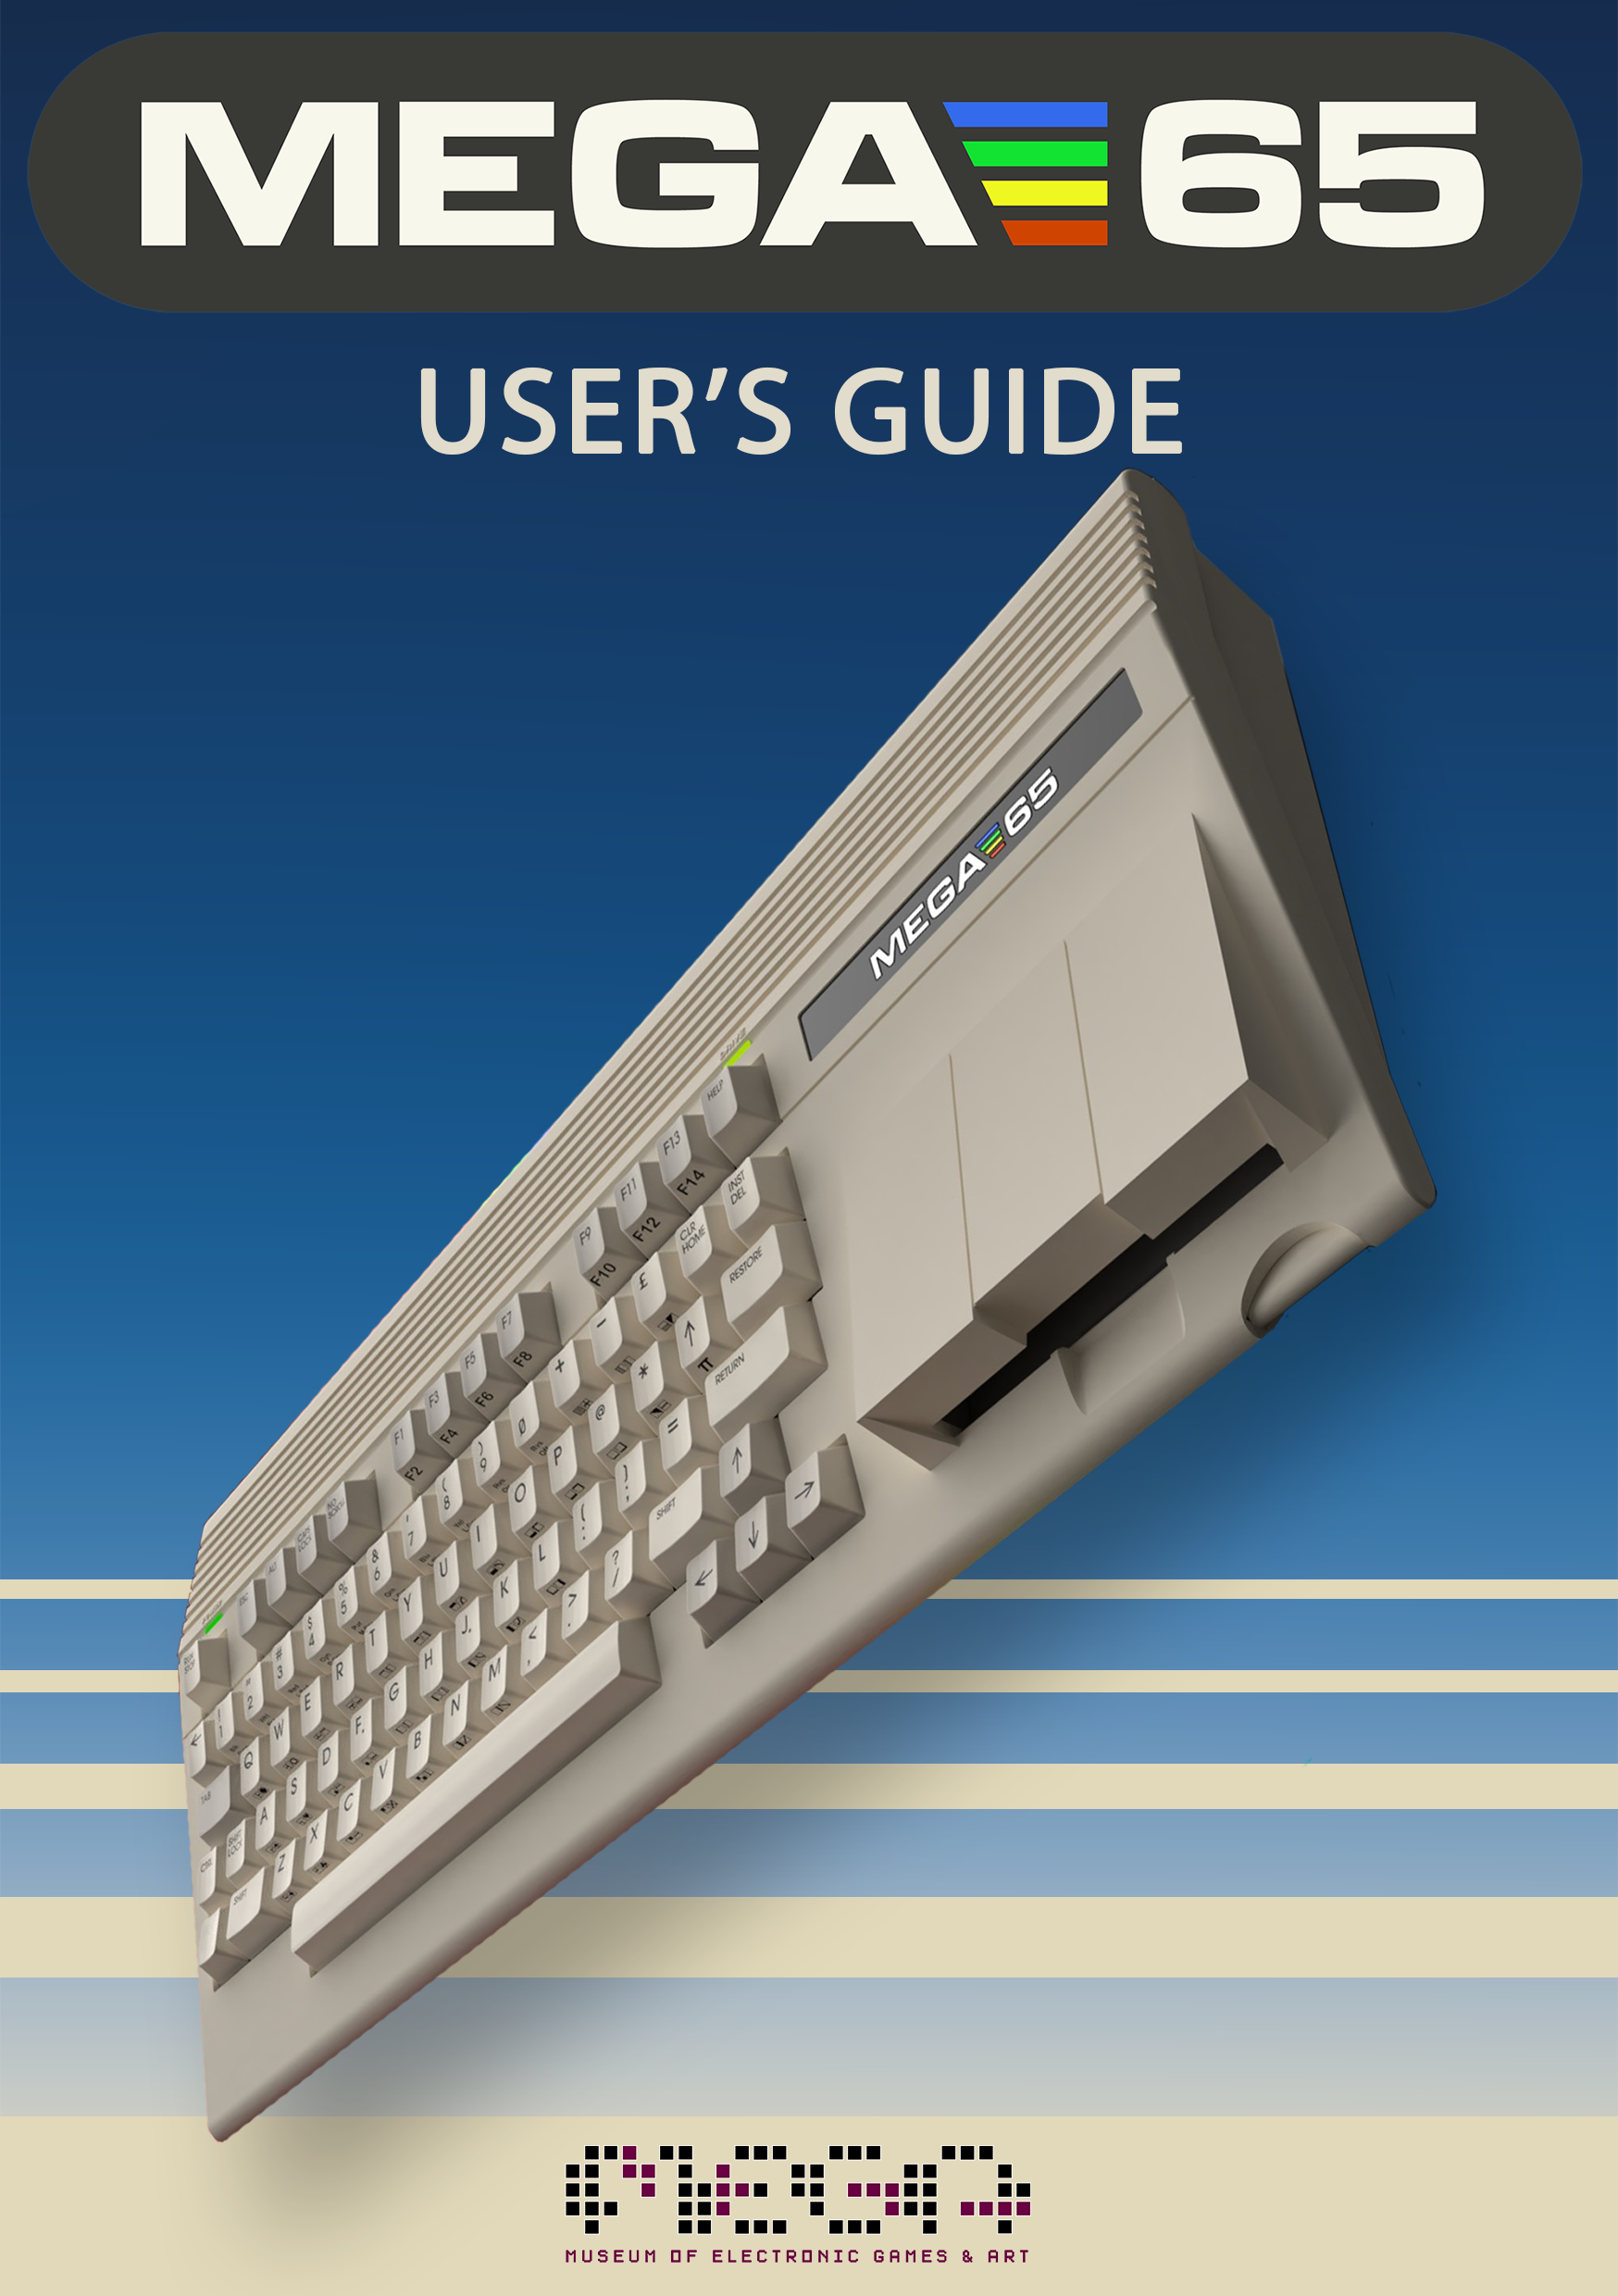
\includegraphics[height=210mm,width=149mm]{frontcover/manual_title}};
\end{tikzpicture}

%\newpage
%\pagecolor{white}

%\vspace*{-2cm}\chapter*{MEGA65 TEAM}
\newpage
{\huge MEGA65 TEAM}\vspace{1cm}

\setlength{\tabcolsep}{1mm}
\begin{tabular}{ll}

{\large\bf Dr. Paul Gardner-Stephen}    & {\large\bf Detlef Hastik} \\
\textit{(highlander)}                   & \textit{(deft)} \\
Founder                                 & Co-Founder \\
Software and Virtual Hardware Architect & General Manager \\
Spokesman and Lead Scientist            & Marketing \& Sales \\
& \\
{\large\bf Martin Streit}               & {\large\bf Anton Schneider-Michallek} \\
 \textit{(seriously)}                   & \textit{(adtbm)} \\
Video and Photo Production              & Hardware Pool Management \\
Tax and Organization                    & Soft-, Hard- and V-Hardware Testing \\
Social Media                            & Forum Administration \\
& \\
{\large\bf Falk Rehwagen}               & {\large\bf Antti Lukats} \\
 \textit{(bluewaysw)}                   & \textit{(antti-brain)} \\
Jenkins Build Automation                & Host Hardware Design and Production \\
GEOS, Hardware Quality Management       & \\
& \\
{\large\bf Dieter Penner}               & {\large\bf Dr. Edilbert Kirk} \\
 \textit{(doubleflash)}                 & \textit{(Bit Shifter)} \\
Host Hardware Review and Testing        & Manual and Tools \\
File Hosting                            & ROM Enhancements \\
& \\
{\large\bf Gábor Lénárt}                & {\large\bf Mirko H.} \\
 \textit{(LGB)}                         & \textit{(sy2002)} \\
Emulator                                & Additional Hardware and Platforms \\
& \\
{\large\bf Farai Aschwanden}            & {\large\bf Thomas Hertzler} \\
 \textit{(Tayger)}                      & \textit{(grumpyninja)} \\
File Base, Tools                        & USA Spokesman \\
Financial Advisory                      & Artist Relations \\
& \\
{\large\bf Andrew Owen}                 & {\large\bf Daniel England} \\
 \textit{(Cheveron)}                    & \textit{(Mew Pokémon)} \\
Keyboard Advisory, Sinclair Support     & Additional Code and Tools \\
& \\
{\large\bf Roman Standzikowski}         & {\large\bf Hernán Di Pietro} \\
 \textit{(FeralChild)}                  & \textit{(indiocolifa)} \\
Open ROMs                               & Additional Emulation \\
\end{tabular}


\chapter*{Reporting Errors and Omissions}

This book is a work-in-progress produced by and for the MEGA65 community.
The version of this edition is:

\input{gitinfo}

We want this book to be the best that it possibly can. So if you see any errors,
find anything that is missing, or would like more information,
please report them using the MEGA65 User's Guide issue tracker:

\url{https://github.com/mega65/mega65-user-guide/issues}

You can also check there to see if anyone else has reported a similar problem,
while you wait for this book to be updated.

Finally, you can always download the latest version of this book from:

\url{https://github.com/mega65/mega65-user-guide}




% paper title
% Titles are generally capitalised except for words such as a, an, and, as,
% at, but, by, for, in, nor, of, on, or, the, to and up, which are usually
% not capitalised unless they are the first or last word of the title.
% Linebreaks \\ can be used within to get better formatting as desired.
% Do not put math or special symbols in the title.

\cleardoublepage

\pagenumbering{roman}

  \begin{titlepage}
    \pagecolor{blue}
     \begin{center}
       {
         \large
         % Put a nice amount of vertical space before the title
         \vspace*{2cm}
               {\Huge\textcolor{white}{\bf{MEGA65 CHIPSET REFERENCE}}}\\
             \vspace{\fill}
                    {\textcolor{white}
                    {Published by \\ the MEGA Museum of Electronic Games \& Art e.V., Germany.}}
       }
     \end{center}
   \end{titlepage}

% Then the copyright notice page
  \pagecolor{white}\textcolor{black}
  \vfill
  WORK IN PROGRESS

  \index{copyright}Copyright \copyright 2019 -- 2021 by Paul Gardner-Stephen,
  the MEGA Museum of Electronic Games \& Art e.V.,
  and contributors.

  This reference guide is made available under the GNU Free Documentation
  License v1.3, or later, if desired. This means that you are free to
  modify, reproduce and redistribute this reference guide, subject to
  certain conditions. The full text of the GNU Free Documentation
  License v1.3 can be found at
  \url{https://www.gnu.org/licenses/fdl-1.3.en.html}.

  Implicit in this copyright license, is the permission to duplicate
  and/or redistribute this document in whole or in part for use in
  education environments. We want to support the education of future
  generations, so if you have any worries or concerns, please contact us.

   \par\today

\newpagestyle{onlynumber}{\setfoot[][{\bf\small\thepage}][]
                                  {} {\bf\small\thepage} {}}
\pagestyle{onlynumber}
\pagecolor{white}

\tableofcontents

%% XXX - big numbers are not in bold, because latex gets confused
\newcommand*{\justifyheading}{\raggedleft}
\definecolor{headingblue}{rgb}{0.5,0.5,1}

% \titleformat{command}[shape]
%   {format}
%   {label}
%   {sep}
%   {before}
%   [after]

% ***************
% PART title page
% ***************

\titleclass{\part}{top}
\titleformat{\part}[display]
   {\thispagestyle{empty}\pagecolor{blue}\normalfont\huge\bfseries\justifyheading}
   {\textcolor{white}{\fontsize{50}{65}\selectfont\bf{PART}\quad{\fontsize{100}{130}\selectfont \bf{\serifed\thepart}}}}
   {20pt}
   {\Huge\textcolor{white}}
   [\newpage\pagecolor{white}\textcolor{black}]

% ******************
% CHAPTER title page
% ******************

\titleformat{\chapter}[display]
   {\thispagestyle{empty}\pagecolor{blue}\normalfont\huge\bfseries\justifyheading}
   {\textcolor{white}{\MakeUppercase{\chaptertitlename}\quad{\fontsize{100}{130}\selectfont \bf\thechapter}}}
   {20pt}
   {\Huge\textcolor{white}}
   [{\chapmtoc\insertminitoc}\newpage\pagecolor{white}\textcolor{black}\cleardoublepage]

% ******************
% SECTION title page
% ******************

\titleformat{\section}[display]
   {\raggedright}
   {\thesection}
   {20pt}
   {\huge\bf\color{headingblue}\uppercase}
   [\color{black}]

\cleardoublepage
\pagenumbering{arabic}

  \chapter{System Memory Map}
\label{cha:memory-map}
\section{Introduction}

The MEGA65 computer has a large 28-bit address space, which allows it
to address up to 256MB of memory and memory-mapped devices.
This memory map has several different views, depending on which mode
the computer is operating in. Broadly, there are five main modes:
(1) Hypervisor mode; (2) C64 compatibility mode; (3) C65 compatibility mode; (4) UltiMAX
compatibility mode; and (5) MEGA65-mode, or one of the other modes,
where the programmer has made use of MEGA65 enhanced features.

It is important to understand that, unlike the C128, the C65 and
MEGA65 allow access to all enhanced features from C64-mode, if the
programmer wishes to do so.  This means that while we frequently talk
about ``C64-mode,'' ``C65-mode'' and ``MEGA65-mode,'' these are simply
terms of convenience for the MEGA65 with its memory map (and sometimes
other features) configured to provide an environment that matches
the appropriate mode.  The heart of this is the MEGA65's flexible
memory map.

In this appendix, we will begin by describing the MEGA65's native
memory map, that is, where all of the memory, I/O devices and other
features appear in the 28-bit address space. We will then explain how
C64 and C65 compatible memory maps are accessed from this 28-bit
address space.

\newpage

\section{MEGA65 Native Memory Map}

\subsection{The First Sixteen 64KB Banks}

The MEGA65 uses a similar memory map to that of the C65 for the first
MB of memory, i.e., 16 memory banks of 64KB each.
This is because the C65's 4510 CPU can access only 1MB
of address space.  These banks can be accessed from BASIC 65 using the
\stw{BANK}\index{BASIC 65 Commands!BANK},
\stw{DMA}\index{BASIC 65 Commands!DMA}, \stw{PEEK} and \stw{POKE}
commands.  The following table summarises the contents of the first
16 banks:

\setlength{\tabcolsep}{3pt}
\begin{longtable}{|L{1cm}|L{1.5cm}|L{2cm}|p{6cm}|}
\hline
{\bf{HEX}} & {\bf{DEC}} & {\bf{Address}} & {\bf{Contents}} \\
\hline
\endfirsthead
\multicolumn{4}{l@{}}{\ldots continued}\\
\hline
{\bf{HEX}} & {\bf{DEC}} & {\bf{Address}} & {\bf{Contents}} \\
\endhead
\multicolumn{4}{l@{}}{continued \ldots}\\
\endfoot
\hline
\endlastfoot
\hline
\small 0 & \small 0 & \$0xxxx & \multicolumn{1}{p{6cm}|}{First 64KB RAM. This is the RAM visible in C64-mode.}\\
\hline
\small 1 & \small 1 & \$1xxxx & \multicolumn{1}{p{6cm}|}{Second 64KB RAM. This is the 2nd 64KB of RAM present on a C65.}\\
\hline
\small 2 & \small 2 & \$2xxxx & \multicolumn{1}{p{6cm}|}{First half of C65 ROM (C64-mode and shared components) {\em or} RAM}\\
\hline
\small 3 & \small 3 & \$3xxxx & \multicolumn{1}{p{6cm}|}{Second half of C65 ROM (C65-mode components) {\em or} RAM}\\
\hline
\small 4 & \small 4 & \$4xxxx & \multicolumn{1}{p{6cm}|}{Additional RAM (384KB or larger chip-RAM models)}\\
\hline
\small 5 & \small 5 & \$5xxxx & \multicolumn{1}{p{6cm}|}{Additional RAM (384KB or larger chip-RAM models)}\\
\hline
\small 6 & \small 6 & \$6xxxx & \multicolumn{1}{p{6cm}|}{Additional RAM (512KB or larger chip-RAM models)}\\
\hline
\small 7 & \small 7 & \$7xxxx & \multicolumn{1}{p{6cm}|}{Additional RAM (512KB or larger chip-RAM models)}\\
\hline
\small 8 & \small 8 & \$8xxxx & \multicolumn{1}{p{6cm}|}{Additional RAM (1MB or larger chip-RAM models)}\\
\hline
\small 9 & \small 9 & \$9xxxx & \multicolumn{1}{p{6cm}|}{Additional RAM (1MB or larger chip-RAM models)}\\
\hline
\small A & \small 10 & \$Axxxx & \multicolumn{1}{p{6cm}|}{Additional RAM (1MB or larger chip-RAM models)}\\
\hline
\small B & \small 11 & \$Bxxxx & \multicolumn{1}{p{6cm}|}{Additional RAM (1MB or larger chip-RAM models)}\\
\hline
\small C & \small 12 & \$Cxxxx & \multicolumn{1}{p{6cm}|}{Additional RAM (1MB or larger chip-RAM models)}\\
\hline
\small D & \small 13 & \$Dxxxx & \multicolumn{1}{p{6cm}|}{Additional RAM (1MB or larger chip-RAM models)}\\
\hline
\small E & \small 14 & \$Exxxx & \multicolumn{1}{p{6cm}|}{Additional RAM (1MB or larger chip-RAM models)}\\
\hline
\small F & \small 15 & \$Fxxxx & \multicolumn{1}{p{6cm}|}{Additional RAM (1MB or larger chip-RAM models)}\\
\hline
\end{longtable}

The key features of this address space are the 128KB of RAM in the first two banks, which is also present on
the C65. If you intend to write programs which can also run on a C65, you should only use these two banks
of RAM.

On all models it is possible to use all or part of the 128KB of ``ROM'' space as RAM. To do this, you must first
request that the Hypervisor removes the read-only protection on this area, before you will be able to change
its contents.  If you are writing a program which will start from C64-mode, or otherwise switch to using the C64
part of the ROM, instead of the C65 part), then the second half of that space, i.e., BANK 3, can be safely used
for your programs. This gives a total of 192KB of RAM, which is available on all models of the MEGA65.

On models that have 384KB or more of chip RAM, BANK 4 and 5 are also available.  Similarly, models which provide
1MB or more of chip RAM will have BANK 6 through 15 also available, giving a total of 896KB (or 960KB, if only
the C64 part of the ROM is required) of RAM available for your programs.  Note that the MEGA65's built-in
freeze cartridge currently freezes only the first 384KB of RAM.

\subsection{Colour RAM}

The MEGA65's VIC-IV video controller supports much larger screens than the VIC-II or VIC-III. For this reason, it
has access to a separate colour RAM, similar to on the C64.  For compatibility with the C65, the first two kilo-bytes
of this are accessible at \$1F800 -- \$1FFFF.  The full 32KB or 64KB of colour RAM is located at \$FF80000.
This is most easily access through the use of advanced DMA operations, or the 32-bit base-page indirect addressing
mode of the processor.

At the time of writing, the \stw{BANK} and \stw{DMA} commands cannot be used to access the rest of the colour RAM, because the
colour RAM is not located in the first mega-byte of address space.  This may be corrected in a future revision of
the MEGA65, allowing access to the full colour RAM via BANK 15 or an equivalent DMA job.

\subsection{28-bit Address Space}

In addition to the C65-style 1MB address space, the MEGA65 extends this
to 256MB, by using 28-bit addresses.  The following shows the high-level
layout of this address space.

\setlength{\tabcolsep}{3pt}
\begin{longtable}{|L{1.5cm}|L{2cm}|L{1.1cm}|p{6cm}|}
\hline
{\bf{HEX}} & {\bf{DEC}} & {\bf{Size}} & {\bf{Contents}} \\
\hline
\endfirsthead
\multicolumn{3}{l@{}}{\ldots continued}\\
\hline
{\bf{HEX}} & {\bf{DEC}} & {\bf{Size}} & {\bf{Contents}} \\
\endhead
\multicolumn{3}{l@{}}{continued \ldots}\\
\endfoot
\hline
\endlastfoot
\hline
\small 0000000 & \small 0 & 1 & \multicolumn{1}{p{6cm}|}{CPU I/O Port Data
  Direction Register}\\
\hline
\small 0000001 & \small 1 & 1 & \multicolumn{1}{p{6cm}|}{CPU I/O Port Data}\\
\hline
\small 0000002 -- 005FFFF & \small 2 -- 384KB & 384KB &
\multicolumn{1}{p{6cm}|}{Fast chip RAM (40MHz)}\\
\hline
\small 0060000 -- 0FFFFFF & \small 384KB -- 16MB  & 15.6MB &
\multicolumn{1}{p{6cm}|}{Reserved for future chip RAM expansion}\\
\hline
\small 1000000 -- 3FFFFFF & \small 16MB -- 64MB & 48MB &
\multicolumn{1}{p{6cm}|}{Reserved}\\
\hline
\small 4000000 -- 7FFFFFF & \small 64MB -- 128MB & 64MB &
\multicolumn{1}{p{6cm}|}{Cartridge port and other devices on the slow bus
  (1 -- 10 MHz)}\\
\hline
\small 8000000 -- 87FFFFF & \small 128MB -- 135MB & 8MB &
\multicolumn{1}{p{6cm}|}{8MB ATTIC RAM (selected models only)}\\
\hline
\small 8800000 -- 8FFFFFF & \small 135MB -- 144MB & 8MB &
\multicolumn{1}{p{6cm}|}{8MB CELLAR RAM (selected models only)}\\
\hline
\small 9000000 -- EFFFFFF & \small 144MB -- 240MB & 96MB &
\multicolumn{1}{p{6cm}|}{Reserved for future expansion RAM}\\
\hline
\small F000000 -- FF7DFFF & \small 240MB -- 255.49MB & 15.49MB &
\multicolumn{1}{p{6cm}|}{Reserved for future I/O expansion}\\
\hline
\small FF7E000 -- FF7EFFF & \small 255.49MB -- 255.49MB & 4KB &
\multicolumn{1}{p{6cm}|}{VIC-IV Character ROM (write only)}\\
\hline
\small FF80000 -- FF87FFF & \small 255.5MB -- 255.53MB & 32KB &
\multicolumn{1}{p{6cm}|}{VIC-IV Colour RAM (32KB colour RAM models)}\\
\hline
\small FF88000 -- FF8FFFF & \small 255.53MB -- 255.57MB & 32KB &
\multicolumn{1}{p{6cm}|}{Additional VIC-IV Colour RAM (64KB colour RAM models only)}\\
\hline
\small FF90000 -- FFCAFFF & \small 255.53MB -- 255.80MB & 216KB &
\multicolumn{1}{p{6cm}|}{Reserved}\\
\hline
\small FFCB000 -- FFCBFFF & \small 255.80MB -- 255.80MB & 4KB &
\multicolumn{1}{p{6cm}|}{Emulated C1541 RAM}\\
\hline
\small FFCC000 -- FFCFFFF & \small 255.80MB -- 255.81MB & 16KB &
\multicolumn{1}{p{6cm}|}{Emulated C1541 ROM}\\
\hline
\small FFD0000 -- FFD0FFF & \small 255.81MB -- 255.81MB & 4KB &
\multicolumn{1}{p{6cm}|}{C64 \$Dxxx I/O Personality}\\
\hline
\small FFD1000 -- FFD1FFF & \small 255.81MB -- 255.82MB & 4KB &
\multicolumn{1}{p{6cm}|}{C65 \$Dxxx I/O Personality}\\
\hline
\small FFD2000 -- FFD2FFF & \small 255.82MB -- 255.82MB & 4KB &
\multicolumn{1}{p{6cm}|}{MEGA65 \$Dxxx Ethernet I/O Personality}\\
\hline
\small FFD3000 -- FFD3FFF & \small 255.82MB -- 255.82MB & 4KB &
\multicolumn{1}{p{6cm}|}{MEGA65 \$Dxxx Normal I/O Personality}\\
\hline
\small FFD4000 -- FFD5FFF & \small 255.82MB -- 255.83MB & 8KB &
\multicolumn{1}{p{6cm}|}{Reserved}\\
\hline
\small FFD6000 -- FFD67FF & \small 255.83MB -- 255.83MB & 2KB &
\multicolumn{1}{p{6cm}|}{Hypervisor scratch space}\\
\hline
\small FFD6000 -- FFD6BFF & \small 255.83MB -- 255.83MB & 3KB &
\multicolumn{1}{p{6cm}|}{Hypervisor scratch space}\\
\hline
\small FFD6C00 -- FFD6DFF & \small 255.83MB -- 255.83MB & 512 &
\multicolumn{1}{p{6cm}|}{F011 floppy controller sector buffer}\\
\hline
\small FFD6E00 -- FFD6FFF & \small 255.83MB -- 255.83MB & 512 &
\multicolumn{1}{p{6cm}|}{SD Card controller sector buffer}\\
\hline
\small FFD7000 -- FFD70FF & \small 255.83MB -- 255.83MB & 256 &
\multicolumn{1}{p{6cm}|}{MEGAphone r1 I2C peripherals}\\
\hline
\small FFD7100 -- FFD71FF & \small 255.83MB -- 255.83MB & 256 &
\multicolumn{1}{p{6cm}|}{MEGA65 r2 I2C peripherals}\\
\hline
\small FFD7200 -- FFD72FF & \small 255.83MB -- 255.83MB & 256 &
\multicolumn{1}{p{6cm}|}{MEGA65 HDMI I2C registers (only for models fitted
  with the ADV7511 HDMI driver chip)}\\
\hline
\small FFD7300 -- FFD7FFF & \small 255.83MB -- 255.84MB & 3.25KB &
\multicolumn{1}{p{6cm}|}{Reserved for future I2C peripherals}\\
\hline
\small FFD8000 -- FFDBFFF & \small 255.83MB -- 255.86MB & 16KB &
\multicolumn{1}{p{6cm}|}{Hypervisor ROM (only visible in Hypervisor Mode)}\\
\hline
\small FFDC000 -- FFDDFFF & \small 255.86MB -- 255.87MB & 8KB &
\multicolumn{1}{p{6cm}|}{Reserved for Hypervisor Mode ROM expansion}\\
\hline
\small FFDE000 -- FFDE7FF & \small 255.87MB -- 255.87MB & 2KB &
\multicolumn{1}{p{6cm}|}{Reserved for Ethernet buffer expansion}\\
\hline
\small FFDE800 -- FFDEFFF & \small 255.87MB -- 255.87MB & 2KB &
\multicolumn{1}{p{6cm}|}{Ethernet frame read buffer (read only) and
  Ethernet frame write buffer (write only)}\\
\hline
\small FFDF000 -- FFDFFFF & \small 255.87MB -- 255.87MB & 4KB &
\multicolumn{1}{p{6cm}|}{Virtual FPGA registers (selected models only)}\\
\hline
\small FFE0000 -- FFFFFFF & \small 255.87MB -- 256MB & 128KB &
\multicolumn{1}{p{6cm}|}{Reserved}\\
\hline
\end{longtable}

\section{\$D000 -- \$DFFF I/O Personalities}
\label{sec:iopersonalities}

The MEGA65 supports four different I/O personalities.  These are
selected by writing the appropriate values to the \$D02F KEY register,
which is visible in all four I/O personalities.  There is more information in
\bookvref{cha:modes} about the use of the KEY
register.

The following table shows which I/O devices are visible in each of
these I/O modes, as well as the KEY register values that are used to
select the I/O personality.

\newpage
\setlength{\tabcolsep}{3pt}
\begin{longtable}{|p{2.2cm}|C{2cm}|C{2cm}|C{2cm}|C{2cm}|}
\hline
{\bf{HEX}} & {\bf{C64}} & {\bf{C65}} & {\bf{MEGA65 ETHERNET}} & {\bf{MEGA65}} \\
\hline
\endfirsthead
\multicolumn{3}{l@{}}{\ldots continued}\\
\hline
{\bf{HEX}} & {\bf{C64}} & {\bf{C65}} & {\bf{MEGA65 ETHERNET}} & {\bf{MEGA65}} \\
\endhead
\multicolumn{3}{l@{}}{continued \ldots}\\
\endfoot
\multicolumn{5}{p{10.2cm}}{{$^1$} In the C64 I/O personality, \$D030 behaves as on C128, allowing toggling
  between 1MHz and 2MHz CPU speed.}\\
\multicolumn{5}{p{10.2cm}}{{$^2$} The additional MEGA65 SIDs are visible in
  all I/O personalities.}\\
\multicolumn{5}{p{10.2cm}}{{$^3$} Some models may replace the repeated images
  of the first four SIDs with four additional SIDs, for a total of 8 SIDs.}\\
\endlastfoot
\hline
\small KEY & \small \$00 & \$A5, \$96 & \$45, \$54  & \$47, \$53 \\
\hline
\small \$D000 -- \$D02F & \small VIC-II & VIC-II & VIC-II & VIC-II \\
\hline
\small \$D030 -- \$D07F & \small VIC-II{$^1$} & VIC-III & VIC-III & VIC-III \\
\hline
\small \$D080 -- \$D08F & \small VIC-II & F011 & F011 & F011 \\
\hline
\small \$D090 -- \$D09F & \small VIC-II & -- & SD card & SD card \\
\hline
\small \$D0A0 -- \$D0FF & \small VIC-II & RAM EXPAND CONTROL & -- & -- \\
\hline
\small \$D100 -- \$D1FF & \small VIC-II & RED Palette & RED Palette &
RED Palette \\
\hline
\small \$D200 -- \$D2FF & \small VIC-II & GREEN Palette & GREEN Palette &
GREEN Palette \\
\hline
\small \$D300 -- \$D3FF & \small VIC-II & BLUE Palette & BLUE Palette &
BLUE Palette \\
\hline
\small \$D400 -- \$D41F & \small SID Right \#1 & SID Right \#1 & SID Right \#1 &
SID Right \#1 \\
\hline
\small \$D420 -- \$D43F & \small SID Right \#2 & SID Right \#2 & SID Right \#2 &
SID Right \#2 \\
\hline
\small \$D440 -- \$D45F & \small SID Left \#1 & SID Left \#1 & SID Left \#1 &
SID Left \#1 \\
\hline
\small \$D460 -- \$D47F & \small SID Left \#2 & SID Left \#2 & SID Left \#2 &
SID Left \#2 \\
\hline
\small \$D480 -- \$D49F & \small SID Right \#1 & SID Right \#1 & SID Right \#1 &
SID Right \#1 \\
\hline
\small \$D4A0 -- \$D4BF & \small SID Right \#2 & SID Right \#2 & SID Right \#2 &
SID Right \#2 \\
\hline
\small \$D4C0 -- \$D4DF & \small SID Left \#1 & SID Left \#1 & SID Left \#1 &
SID Left \#1 \\
\hline
\small \$D4E0 -- \$D4FF & \small SID Left \#2 & SID Left \#2 & SID Left \#2 &
SID Left \#2 \\
\hline
\small \$D500 -- \$D5FF & \small SID images & -- & Reserved & Reserved \\
\hline
\small \$D600 -- \$D63F & \small -- & UART & UART & UART \\
\hline
\small \$D640 -- \$D67F & \small -- & UART images & HyperTrap
Registers & HyperTrap Registers \\
\hline
\small \$D680 -- \$D6FF & \small -- & -- & MEGA65 Devices & MEGA65 Devices \\
\hline
\small \$D700 -- \$D7FF & \small -- & -- & MEGA65 Devices & MEGA65 Devices \\
\hline
\small \$D800 -- \$DBFF & \small COLOUR RAM & COLOUR RAM & ETHERNET Buffer & COLOUR RAM \\
\hline
\small \$DC00 -- \$DDFF & \small CIAs & CIAs / COLOUR RAM & ETHERNET Buffer & CIAs / COLOUR RAM \\
\hline
\small \$DE00 -- \$DFFF & \small CART I/O & CART I/O & ETHERNET Buffer & CART I/O / SD SECTOR \\
\hline
\end{longtable}

\section{CPU Memory Banking}
\label{sec:membanking}

The 45GS10 processor, like the 6502, can only ``see'' 64KB of memory
at a time. Access to additional memory is via a selection of
bank-switching mechanisms.  For backward-compatibility with the C64
and C65, the memory banking mechanisms for both of these computers
existing the MEGA65:
\begin{enumerate}
\item C65-style MAP instruction banking
\item C65-style \$D030 banking
\item C64-style cartridge banking
\item C64-style \$00 / \$01 banking
\end{enumerate}

It is important to understand that these different banking modes have
a priority order: If a higher priority form of banking is being used,
it takes priority over a lower priority form.  The C65 banking methods
take priority of the C64-mode banking methods.  So, for example, if
the 45GS10 MAP instruction has been used to provide a particular
memory layout, the C64-style \$00 / \$01 banking will not be visible.

This makes the overall banking scheme more complex than on the C64.
Thus to understand what the actual memory layout will be, you should
start by considering the effects of C64 memory banking, and then if
any C65 MAP instruction memory banking is enabled, using that to override the
C64-style memory banking. Then if any C65 \$D030 memory banking is
used, that overrides both the C64 and C65 MAP instruction memory
banking. Finally, if I/O is banked, or if there are any cartridges
inserted and active, their effects are made.

The following diagram shows the different types of banking that can
apply to the different areas of the 64KB that the CPU can see.  The
higher layers take priority over the lower layers, as described in the
previous paragraph.
\begin{center}
\begin{tabular}{rccccccc}
\cline{4-5} \cline{7-8}
\rowcolor[HTML]{C0C0C0} I/O/CART &                                 & \multicolumn{1}{c|}{\cellcolor[HTML]{C0C0C0}}                               & \multicolumn{1}{c|}{\cellcolor[HTML]{FE0000}\begin{tabular}[c]{@{}c@{}}CART\\ ROMLO\end{tabular}} & \multicolumn{1}{c|}{\cellcolor[HTML]{FE0000}\begin{tabular}[c]{@{}c@{}}CART\\ ROMHI\end{tabular}} & \multicolumn{1}{c|}{\cellcolor[HTML]{C0C0C0}}                                                      & \multicolumn{1}{c|}{\cellcolor[HTML]{F8A102}I/O}                                                 & \multicolumn{1}{c|}{\cellcolor[HTML]{FE0000}\begin{tabular}[c]{@{}c@{}}CART \\ ROMHI\end{tabular}} \\ \cline{4-8}
\rowcolor[HTML]{EFEFEF}
C65                                                 &                                 & \multicolumn{1}{c|}{\cellcolor[HTML]{EFEFEF}}                               & \multicolumn{1}{c|}{\cellcolor[HTML]{F8FF00}BASIC}                                                & \multicolumn{1}{c|}{\cellcolor[HTML]{F8FF00}BASIC}                                                & \multicolumn{1}{c|}{\cellcolor[HTML]{F8FF00}\begin{tabular}[c]{@{}c@{}}INTER-\\ FACE\end{tabular}} & \multicolumn{1}{c|}{\cellcolor[HTML]{EFEFEF}}                                                   & \multicolumn{1}{c|}{\cellcolor[HTML]{F8FF00}KERNAL}                                                \\ \cline{2-8}
\rowcolor[HTML]{34FF34}
\multicolumn{1}{r|}{\cellcolor[HTML]{C0C0C0}MAP}    & \multicolumn{2}{c|}{\cellcolor[HTML]{34FF34}\begin{tabular}[c]{@{}c@{}}MAP LO\\ (4 x 8KB slabs)\end{tabular}} & \multicolumn{5}{c|}{\cellcolor[HTML]{34FF34}\begin{tabular}[c]{@{}c@{}}MAP HI\\ (4 x 8KB slabs)\end{tabular}}                                                                                                                                                                                                                                                                                                                                                                                                     \\ \cline{2-8}
\rowcolor[HTML]{EFEFEF}
C64                                                 &                                 &                                                                             & \multicolumn{1}{c|}{\cellcolor[HTML]{EFEFEF}}                                                     & \multicolumn{1}{c|}{\cellcolor[HTML]{00D2CB}BASIC}                                                & \multicolumn{1}{c|}{\cellcolor[HTML]{EFEFEF}}                                                      & \multicolumn{1}{c|}{\cellcolor[HTML]{00D2CB}\begin{tabular}[c]{@{}c@{}}CHAR\\ ROM\end{tabular}} & \multicolumn{1}{c|}{\cellcolor[HTML]{00D2CB}KERNAL}                                                \\ \cline{2-8}
\rowcolor[HTML]{9698ED}
\multicolumn{1}{r|}{\cellcolor[HTML]{C0C0C0}RAM}   & \multicolumn{2}{c|}{\cellcolor[HTML]{9698ED}RAM*}                                                             & \multicolumn{1}{c|}{\cellcolor[HTML]{9698ED}RAM}                                                  & \multicolumn{1}{c|}{\cellcolor[HTML]{9698ED}RAM}                                                  & \multicolumn{1}{c|}{\cellcolor[HTML]{9698ED}RAM}                                                   & \multicolumn{1}{c|}{\cellcolor[HTML]{9698ED}RAM}                                                & \multicolumn{1}{c|}{\cellcolor[HTML]{9698ED}RAM}                                                   \\ \cline{2-8}
\rowcolor[HTML]{EFEFEF}
                                                    & \multicolumn{2}{c}{\cellcolor[HTML]{EFEFEF}\begin{tabular}[c]{@{}c@{}}\$0000 --\\ \$7FFF\end{tabular}}        & \begin{tabular}[c]{@{}c@{}}\$8000 --\\ \$9FFF\end{tabular}                                        & \begin{tabular}[c]{@{}c@{}}\$A000 --\\ \$BFFF\end{tabular}                                        & \begin{tabular}[c]{@{}c@{}}\$C000 --\\ \$CFFF\end{tabular}                                         & \begin{tabular}[c]{@{}c@{}}\$D000 --\\ \$DFFF\end{tabular}                                      & \begin{tabular}[c]{@{}c@{}}\$E000 --\\ \$FFFF\end{tabular}
\end{tabular}
\end{center}

(There are actually a few further complications. For example, if the
cartridge selects the UltiMAX\texttrademark{} game mode, then only the first 4KB
of RAM will be visible, and the remaining address space will be
un-mapped, and able to be supplied by the cartridge.)

For example, using \$D030 to bank in C65
ROM at \$A000, this will take priority over the C64 BASIC 2 ROM at the
same address.

\section{C64/C65 ROM Emulation}

The C64 and C65 use ROM memories to hold the KERNAL and BASIC system.
The MEGA65 is different: It uses 128KB of its 384KB fast chip RAM at
\$20000 - \$3FFFF (banks 2 and 3) to
hold these system programs. This makes it possible to change or upgrade the
``ROM'' that the MEGA65 is running, without having to open the
computer. It is even possible to use the MEGA65's Freeze Menu to
change the ``ROM'' being used while a program is running.

The C64 and C65 memory banking methods use this 128KB of area when
making ROM banks visible.  When the RAM banks are mapped, they are
always read-only.  However, if the MAP instruction or DMA is used to
access that address area, it is possible to write to it. For improved
backward compatibility, the whole 128KB region of memory is normally
set to read-only.

A program can, however, request read-write access to this
128KB area of memory, so that it can make full use of the MEGA65's
384KB of chip RAM.  This is accomplished by triggering the {\em Toggle
  Rom Write-protect} system trap of the hypervisor.  The following
code-fragment demonstrates how to do this. Calling it a second time
will re-activate the write-protection.

\begin{screenoutput}
  LDA #$70
  STA $D640
  NOP
\end{screenoutput}

This fragment works by
calling sub-function \$70 (toggle ROM write-protect) of Hypervisor
trap \$00. Note that the \screentext{NOP} is mandatory. The MEGA65
I/O personality must be first selected, so that the \$D640 register is
un-hidden.

The current write-protection
state can be tested by attempting to write to this area of memory.
Also, you can examine and toggle the current state from in the MEGA65
Freeze Menu.

NOTE: If you are starting your program from C65-mode, you must first make
sure that the I/O area is visible at \$D000-\$DFFF.  The simplest way to do
this is to use the {\tt MAP} instruction with all zero values in the registers.
The following fragment demonstrates this, and also makes sure that the MEGA65 I/O
context is active, so that the hypervisor trap will be able to trigger:

\begin{screenoutput}

  ; Clear C65 memory map
  LDA #$00
  TAX
  TAY
  TAZ
  MAP
  ; Bank I/O in via C64 mechanism
  LDA #$35
  STA $01
  ; Do MEGA65 / VIC-IV I/O knock
  LDA #$47
  STA $D02F
  LDA #$53
  STA $D02F
  ; End MAP sequence, thus allowing interrupts to occur again
  EOM
  ; Do Hypervisor call to un-write-protect the ROM area
  LDA #$70
  STA $D640
  NOP
\end{screenoutput}


\subsection{C65 Compatibility ROM Layout}

The layout of the C65 compatibility 128KB ROM area is identical to that of the C65:

{\ttfamily
\setlength{\tabcolsep}{3pt}
\begin{tabular}{|l|l|}
\hline
{\bf{HEX}} & {\bf{Contents}} \\
\hline
\$3E000 -- \$3FFFF & C65 KERNAL \\
\hline
\$3C000 -- \$3DFFF & RESERVED \\
\hline
\$38000 -- \$3BFFF & C65 BASIC GRAPHICS ROUTINES \\
\hline
\$32000 -- \$37FFF & C65 BASIC \\
\hline
\$30000 -- \$31FFF & MONITOR (gets mapped at \$6000 -- \$7FFF) \\
\hline
\$2E000 -- \$2FFFF & C64 KERNAL \\
\hline
\$2D000 -- \$2DFFF & C64 CHARSET \\
\hline
\$2C000 -- \$2CFFF & INTERFACE \\
\hline
\$24000 -- \$27FFF & RESERVED \\
\hline
\$20000 -- \$23FFF & DOS (gets mapped at \$8000 -- \$BFFF) \\
\hline
\end{tabular}
}

The INTERFACE program is a series of routines that are used by the C65
to switch between C64-mode, C65-mode and the C65's built-in DOS.  The
DOS is located in the lower-eighth of the ROM.





  \chapter{45GS02 Microprocessor}
\label{cha:cpu}
\label{cha:45gs02}
\section{Introduction}

The 45GS02 is an enhanced version of the processor portion of the CSG4510
and of the F018 "DMAgic" DMA controller used in the Commodore 65
computer prototypes.  The 4510 is, in turn,
an enhanced version of the 65CE02.
The reader is referred to
the considerable documentation available for the 6502 and 65CE02 processors
for the backwards-compatible operation of the 45GS02.

This chapter will
focus on the differences between the 45GS02 and the earlier 6502-class
processors, and the documentation of the many built-in memory-mapped I/O
registers of the 45GS02.

\section{Differences to the 6502}

The 45GS02 has a number of key differences to earlier 6502-class processors:

\subsection{Supervisor/Hypervisor Privileged Mode}

Unlike the earlier 6502 variants, the 45GS02 has a privileged mode of operation.
This mode is intended for use by an operating system or type-1
hypervisor.  The ambiguity between
operating system and Hypervisor on the MEGA65 stems from the fact that the operating
system of the MEGA65 is effectively little more than a loader and
task-switcher for C64 and C65
environments, i.e., effectively operating as a hypervisor, but provides
only limited virtualisation
of the hardware.

The key differences between normal and supervisor mode on the MEGA65, are that in
supervisor mode:

\begin{itemize}
\item A special 16KB memory area is mapped to \$8000 - \$BFFF, which is
 used to contain both
 the program and data of the Hypervisor / supervisor program.
 This is normally the Hyppo program.
  This memory is not mappable by any means when the processor is in the
 normal mode (the chip-select
  line to it is inhibited), protecting it from accidental or malicious access.
\item The 64 SYSCALL trap registers in the MEGA65 I/O-mode at
\$D640 - \$D67F are replaced by the
  virtualisation control registers.  These registers allow complete
control over the system, and
  it is their access that truly defines the privilege of the supervisor mode.
  \item The processor always operates at full speed (40MHz) and in the
 4510 processor personality.
\end{itemize}

The Hypervisor Mode is described in more detail later in this appendix.

\subsection{6502 Illegal Opcodes}

The 65C02, 65CE02 and CSG4510 processors extended the original 6502 processor
by using previously unallocated opcodes of the 6502 to provide additional
instructions.  All software that followed the official documentation of the 6502
processor will therefore work on these newer processors, possibly with different
instruction timing.  However, the common practice on the C64 and other home computers
of using undefined opcodes (often called ``illegal opcodes'', although there is no
law against using them), means that many existing programs will not work on these
newer processors.

To alleviate this problem the 45GS02 has the ability to switch processor personalities
between the 4510 and 6502.  The effect is that in 6502 mode, none of the new opcodes of
the 65C02, 65CE02, 4510 or 45GS02 are available, and are replaced with the original,
often strange, behaviour of the undefined opcodes of the 6502.

\begin{qoute}
{\bf WARNING:} This feature is incomplete and untested.  Most undocumented
6502 opcodes do not operate correctly when the 6502
personality is enabled.
\end{quote}

\subsection{Read-Modify-Write Instruction Bug Compatibility}

The 65CE02 processor optimised a group of instructions called the
Read-Modify-Write (RMW) instructions.  For such instructions, such as
INC, that increments the contents of a memory location, the 6502 would
read the original value and then write it back unchanged, before
writing it back with the new increased value.  For most purposes, this
did not cause any problems. However, it turned out to be a fast way to
acknowledge VIC-II interrupts, because writing the original value back
(which the instruction doesn't need to do) acknowledges the interrupt.
This method is faster and uses fewer bytes than any alternative, and so
became widely used in C64 software.

The problem came with the C65 with its 65CE02 derived CSG4510 that
didn't do this extra write
during the RMW instructions.  This made the RMW instructions one cycle
faster, which made
software run slightly faster. Unfortunately, it also meant that a lot
of existing C64 software
simply won't run on a C65, unless the interrupt acknowledgement code in
each program is patched
to work around this problem. This is the single most common reason why
many C64 games and other
software titles won't run on a C65.

Because this problem is so common, the MEGA65's 45GS02 includes bug
compatibility with this
commonly used feature of the original 6502.  It does this by checking
if the target of an RMW
instruction is \$D019, i.e., the interrupt status register of the VIC-II.
If it is, then
the 45GS02 performs the dummy write, allowing many C64 software titles
to run unmodified on the
MEGA65, that do not run on a C65 prototype.  By only performing the
dummy write if the address
is \$D019, the MEGA65 maintains C64 compatibility, without sacrificing
the speed improvement
for all other uses of these instructions.

\subsection{Variable CPU Speed}

The 45GS02 is able to run at ~1MHz, ~2MHz, ~3.5MHz and 40MHz,
to support running software
designed for the C64, C128 in C64-mode, C65 and MEGA65.

\subsubsection{Slow (1MHz -- 3.5MHz) Operation}
In these modes, the 45GS02 processor slows down, so that the same number of instructions
per video frame are executed as on a PAL or NTSC C64, C128 in C64-mode or C65 prototype.
This is to allow existing software to run on the MEGA65 at the correct speed, and with
minimal display problems.  The VIC-IV video controller provides cycle indication pulses
to the 45GS02 that are used to keep time.

In these modes, opcodes take the same number of cycles as an 6502.
However memory accesses within an
instruction are not guaranteed to occur in the same cycle as on a 1MHz 6502.  Normally
the effect is that instructions complete faster, and the processor idles until the
correct number of cycles have passed. This means that timing may be incorrect by up to
7 micro-seconds.  This is not normally a problem, and even many C64 fast loaders will
function correctly. For example, the GEOS\texttrademark{} Graphical Operating System for the C64
can be booted and used from a 1541 connected to the MEGA65's serial port.

However, some advanced VIC-II graphics tricks, such as Variable Screen
Position (VSP) are
highly unlikely to work correctly, due to the uncertainty in timing of the memory write
cycles of instructions.  However, in most cases such problems can be
easily solved by using
the advanced features of the MEGA65's VIC-IV video controller.
For example, VSP is unnecessary
on the MEGA65, because you can set the screen RAM address to any location in memory.

\subsubsection{Full Speed (40MHz) Instruction Timing}

When the MEGA65's processor is operating at full speed
(currently 40MHz), the instruction
timing no longer exactly mirrors the 6502: Instructions that can be
executed in fewer cycles
will do so. For example, branches are typically require fewer instructions on the 45GS02.
There are also some instructions that require more cycles on the 45GS02, in particular the
LDA, LDX, LDY and LDZ instructions. Those instructions typically require one additional cycle.
However as the processor is running at 40MHz, these instructions still execute much more quickly
than on even a C65 or C64 with an accelerator.

\subsubsection{CPU Speed Fine-Tuning}
It is also possible to more smoothly
vary the CPU speed using the {\bf SPEEDBIAS} register located at \$D7FA (55290), when MEGA65 I/O mode
is enabled.  The default value is \$80 (128), which means no bias on the CPU speed.  Higher values
increase the CPU speed, with \$FF meaning $2\times$ the expected speed. Lower values slow
the processor down, with \$00 bring the CPU to a complete stand-still.  Thus the speed can be
varied between $0\times$ and $2\times$ the intended value.

This register is provided to allow tweaking the processor speed in games.

Note that this register has no effect when
the processor is running at full-speed, because it only affects the way in which VIC-IV
video cycle indication pulses are processed by the CPU.

\subsubsection{Direct Memory Access (DMA)}
Direct Memory Access (DMA) is a method for quickly filling, copying or swapping memory regions.
The MEGA65 implements an improved version of the F018 ``DMAgic'' DMA controller of the C65 prototypes.
 Unlike on the C65 prototypes, the DMA controller is part of the CPU on the MEGA65.

Detailed information on how to use the DMA controller and these advanced features can be found in \bookvref{cha:dmagic}

\subsection{Accessing memory between the 64KB and 1MB points}

The C65 included four ways to access memory beyond the 64KB point: three methods
that are limited, specialised or both, and two general-purpose methods. We will first
consider the limited methods, before documenting the general-purpose methods.

\subsubsection{C64-Style Memory Banking}

The first method, is to use the C64-style \$00/\$01 ROM/RAM banking.
This method is very limited, however, as it allows only the banking in
and out of the two 8KB regions that correspond to the C64 BASIC and
KERNAL ROMs.  These are located at \$2A000 and \$2E000 in the 20-bit
C65 address space, i.e., \$002A000 and \$002E000 in the 28-bit address
space of the MEGA65.  It can also provide access to the C64 character ROM
data at \$D000, which is located at \$2D000 in the C65 memory map, and thus \$002D0000 in
the MEGA65 address space.  In addition to being limited to which regions this
method can access, it also only provides read-only access
to these memory regions, i.e., it cannot be used to modify these memory regions.

\subsubsection{VIC-III ``ROM'' Banking}

Similar to the C64-style memory banking, the C65 included the facility
to bank several other regions of the C65's 128KB ROM.  These are banked
in and out using various bits of the VIC-III's \$D030 register:

\setlength{\tabcolsep}{3pt}
\begin{longtable}{|L{1.5cm}|L{1.5cm}|L{1.8cm}|L{1.5cm}|L{2cm}|}
\hline
{\bf{\$D030 Bit}} & {\bf{Signal Name}} & {\bf{20-bit Address}} & {\bf{16-bit Address}} & {\bf{Read-Write Access?}} \\
\hline
\endfirsthead
\multicolumn{3}{l@{}}{\ldots continued}\\
\hline
{\bf{\$D030 Bit}} & {\bf{Signal Name}} & {\bf{20-bit Address}} & {\bf{16-bit Address}} & {\bf{Read-Write Access?}} \\
\endhead
\multicolumn{3}{l@{}}{continued \ldots}\\
 \endfoot
 \hline
\endlastfoot
\small 0 & \small CRAM2K & \$1F800 -- \$1FFFF, \$FF80000 -- \$FF807FF & \$D800 -- \$DFFF & Y \\
 \hline
\small 3 & \small ROM8 & \$38000 -- \$39FFF & \$8000 -- \$9FFF & N \\
 \hline
\small 4 & \small ROMA & \$3A000 -- \$3BFFF & \$A000 -- \$BFFF & N \\
 \hline
\small 5 & \small ROMC & \$2C000 -- \$2CFFF & \$C000 -- \$CFFF & N \\
 \hline
\small 6 & \small CROM9 & \$29000 -- \$29FFF & \$D000 -- \$DFFF & N \\
 \hline
\small 7 & \small ROME & \$3E000 -- \$3FFFF & \$E000 -- \$FFFF & N \\
  \hline
   \end{longtable}

The CRAM2K signal causes the normal 1KB of colour RAM, which is located
at \$1F800 -- \$1FBFF and is visible at \$D800 -- \$DBFF, to instead
be visible from \$D800 -- \$DFFF. That is, the entire range \$1F800 -- \$1FFFF
is visible, and can be both read from and written to.  Unlike on the C64,
the colour RAM on the MEGA65 is always visible as 8-bit bytes.  Also, on
the MEGA65, the colour RAM is 32KB in size, and exists at \$FF80000 -- \$FF87FFF.
The visibility of the colour RAM at \$1F800 -- \$1FFFF is achieved by mirroring
writes to both regions when accessing the colour RAM via this mechanism.


Note that these VIC-III memory banking signals take precedence over the
C64-style memory banking.

\subsubsection{VIC-III Display Address Translator}

The third specialised manner to access to memory above the 64KB point is to use
the VIC-III's Display Address Translator.  Use of this mechanism is documented
in \bookvref{cha:viciv}.

\subsubsection{The MAP instruction}
\label{sec:map-instruction}
\index{MAP}\index{Memory banking}

The first general-purpose means of access to memory is the MAP instruction of the
4510 processor. The MEGA65's 45GS02 processor also supports this mechanism.
This instruction divides the 64KB address of the 6502 into eight blocks of 8KB each.
For each of these blocks, the block may either be accessed normally, i.e., accessing
an 8KB region of the first 64KB of RAM of the system.  Alternatively, each block
may instead be re-mapped (hence the name of the MAP instruction) to somewhere else
in the address space, by adding an offset to the address. Mapped addresses in the
first 32KB use one offset, the lower offset, and the second 32KB uses another, the
upper offset.  Re-mapping of memory using the MAP instruction takes precedence over
the C64-style memory banking, but not the C65's ROM banking mechanism.

The offsets must be a multiple of 256 bytes, and thus consist of 12 bits
in order to allow an arbitrary offset in the 1MB address space of the C65.  As each 8KB
block in a 32KB half of memory can be either mapped or not, this requires one bit per
8KB block.  Thus the processor requires 16 bits of information for each half of memory, for
a total of 32 bits of information.  This is achieved by setting the A and X registers for
the lower half of memory and the Y and Z registers for the upper half of memory, before executing
the MAP instruction.

The MAP instruction copies the contents of these registers into the
processors internal registers that hold the mapping information.  Note that there is no way to
use the MAP instruction to determine the current memory mapping configuration, which somewhat
limits its effectiveness.

The following diagram illustrates how the MAP instruction takes the values of the four A, X, Y and Z
registers, and uses them to compue the upper and lower address offsets, and sets the bank enable bits
for each of the eight 8KB memory regions of the 6502 address space:

\begin{center}
  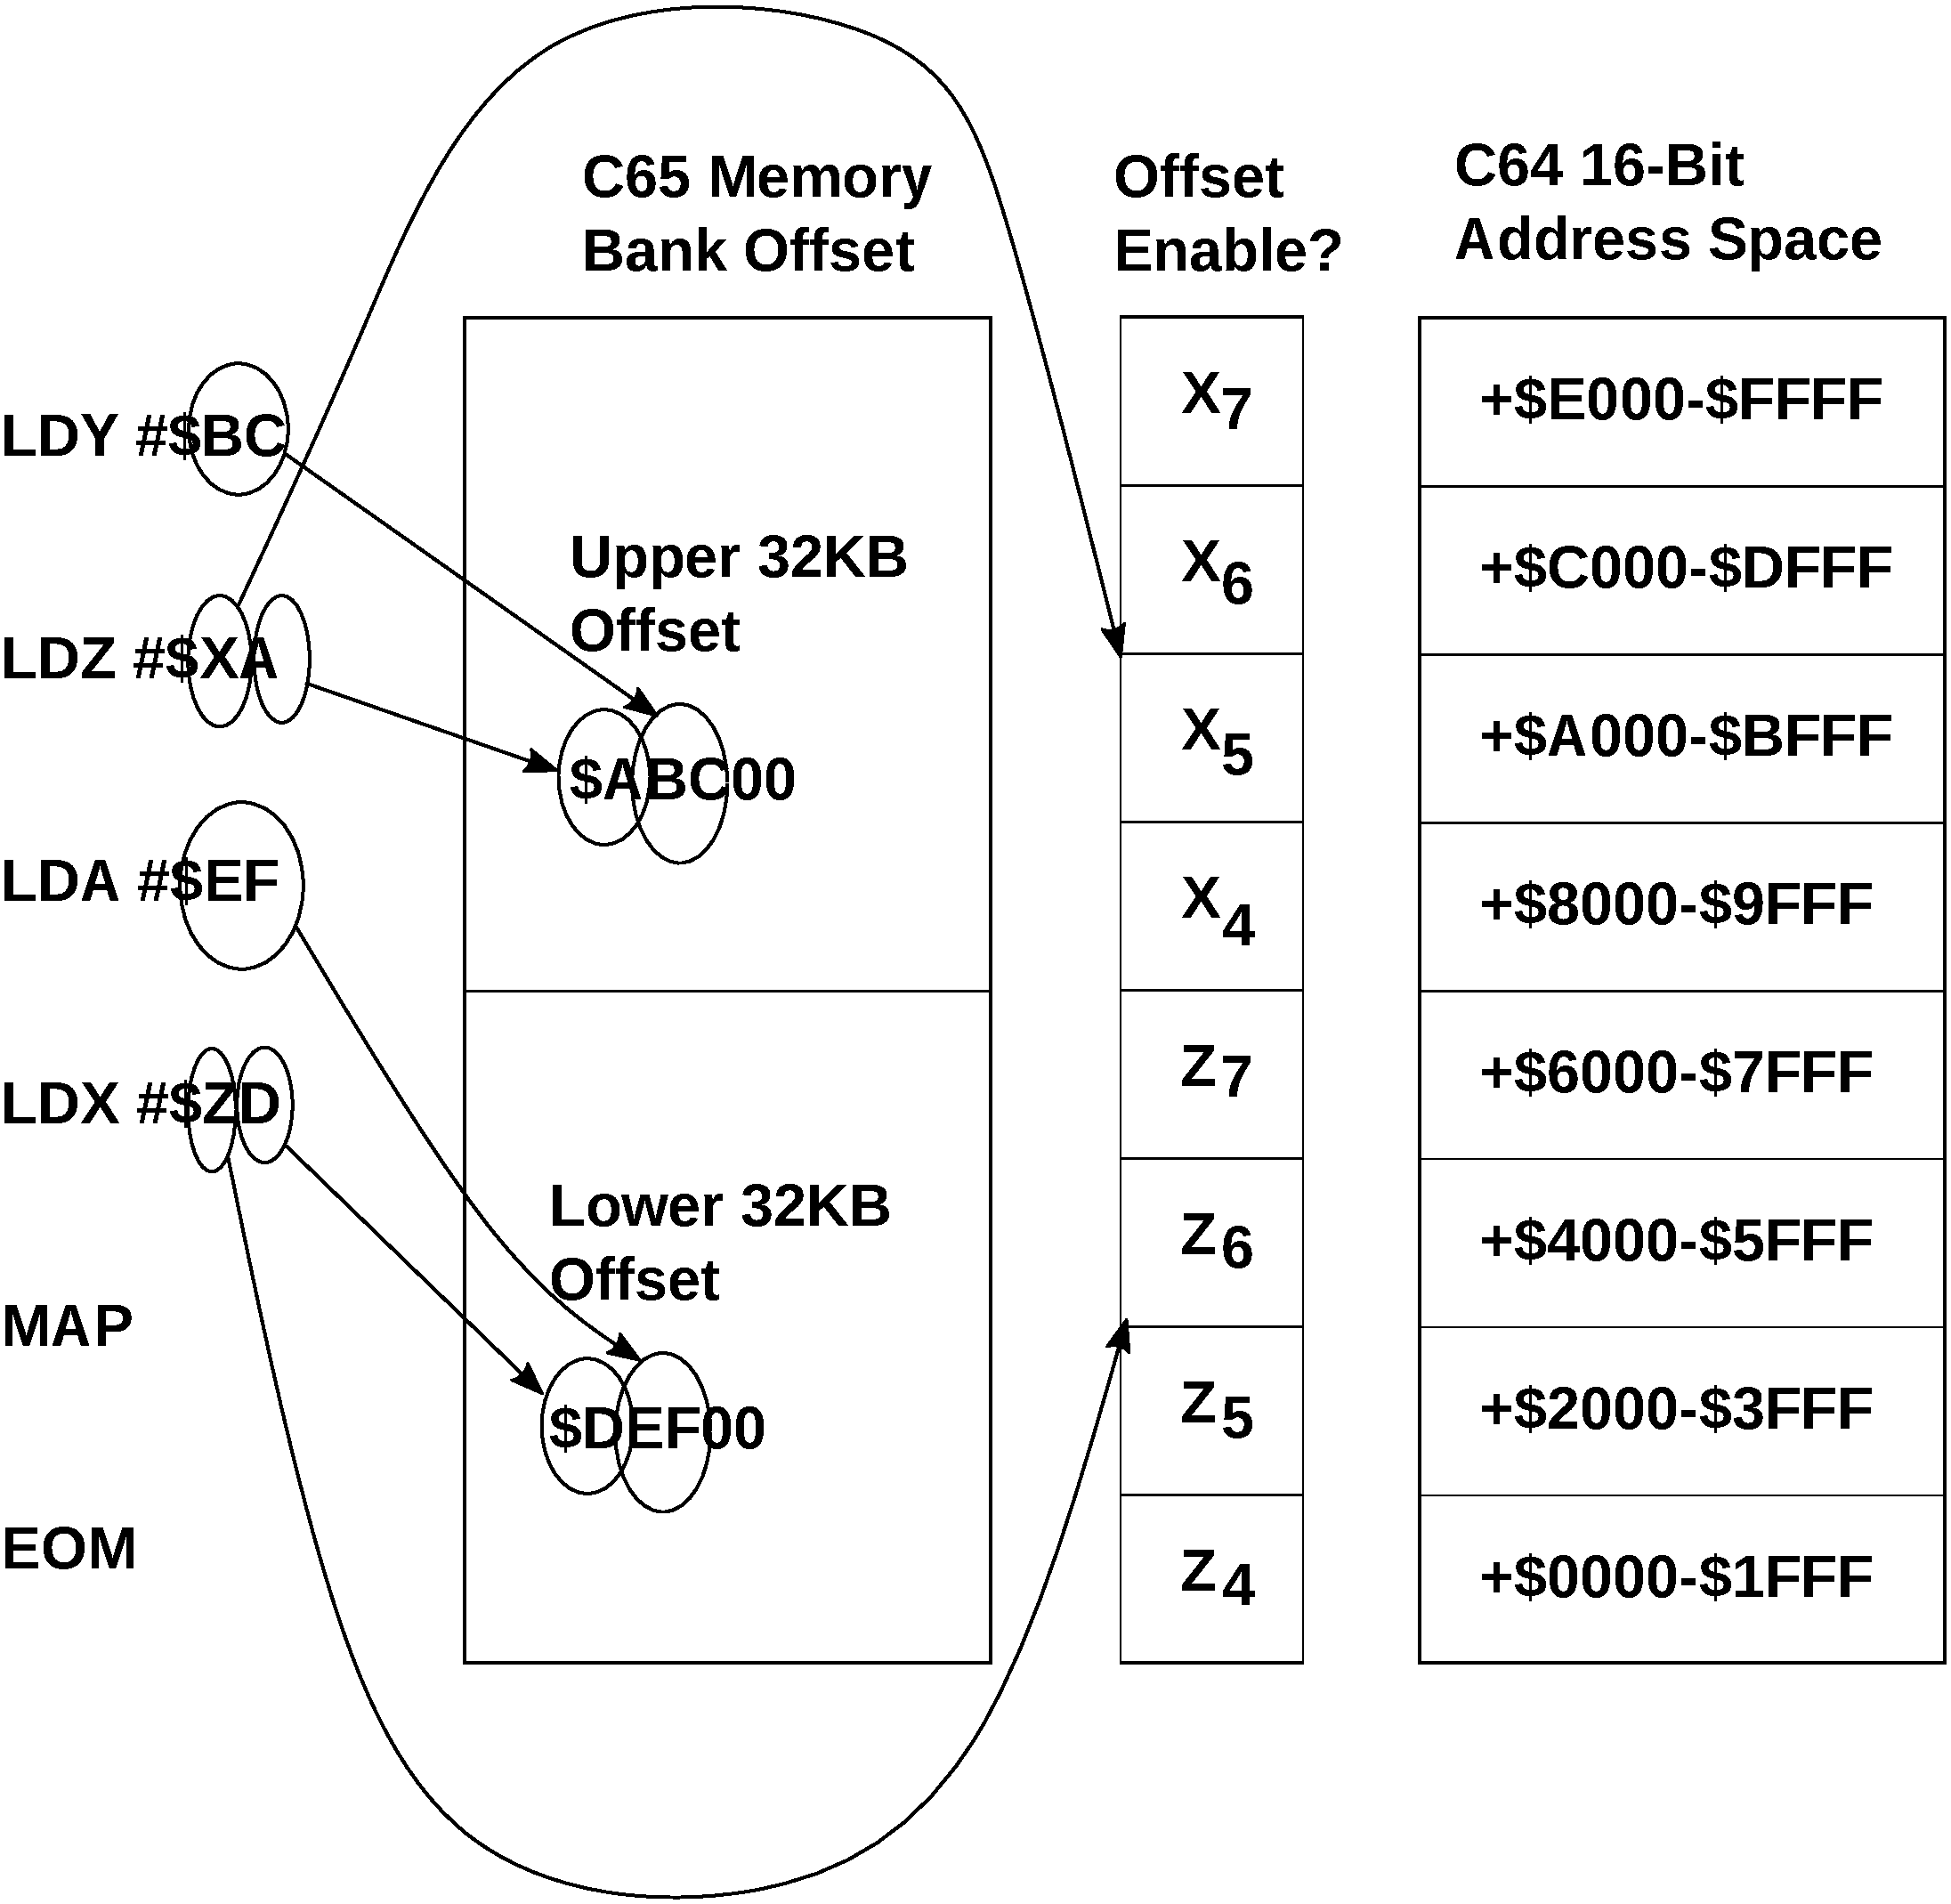
\includegraphics[width=0.75\textwidth]{images/illustrations/map-instruction-operation.pdf}\index{MAP}\index{Memory banking}
\end{center}

That is, the contents of the A register and the lower-nibble of the X register form a 12-bit value
that is multiplied by 256 to produce the offset used for any of the 8KB banks in the lower 32KB half of the 6502's 16-bit address
space.  The upper nibble of the X register is used as flags to indicate which of the four 8KB blocks in that 32KB half of the
6502 address space should have the offset added to their addresses to compute the actual address.

The Y and Z registers are used in a similar way to produce the offset for the upper 32KB half of the 6502 address space, and the
flags to indicate whether the offset is used for each of the four 8KB blocks in that half of the address space.

Note that the lower 8 bits of the offset cannot be set. That is, the offset will be a multiple of 256
bytes, unlike on some extended 6502 processors.  However, in practice this restriction is rarely
limiting.

To understand how this works in practice, the following example shows how this works with a concrete
example, showing the address ranges that would be visible in each of the 8KB slices of the 6502's
64KB address space:

\begin{center}
  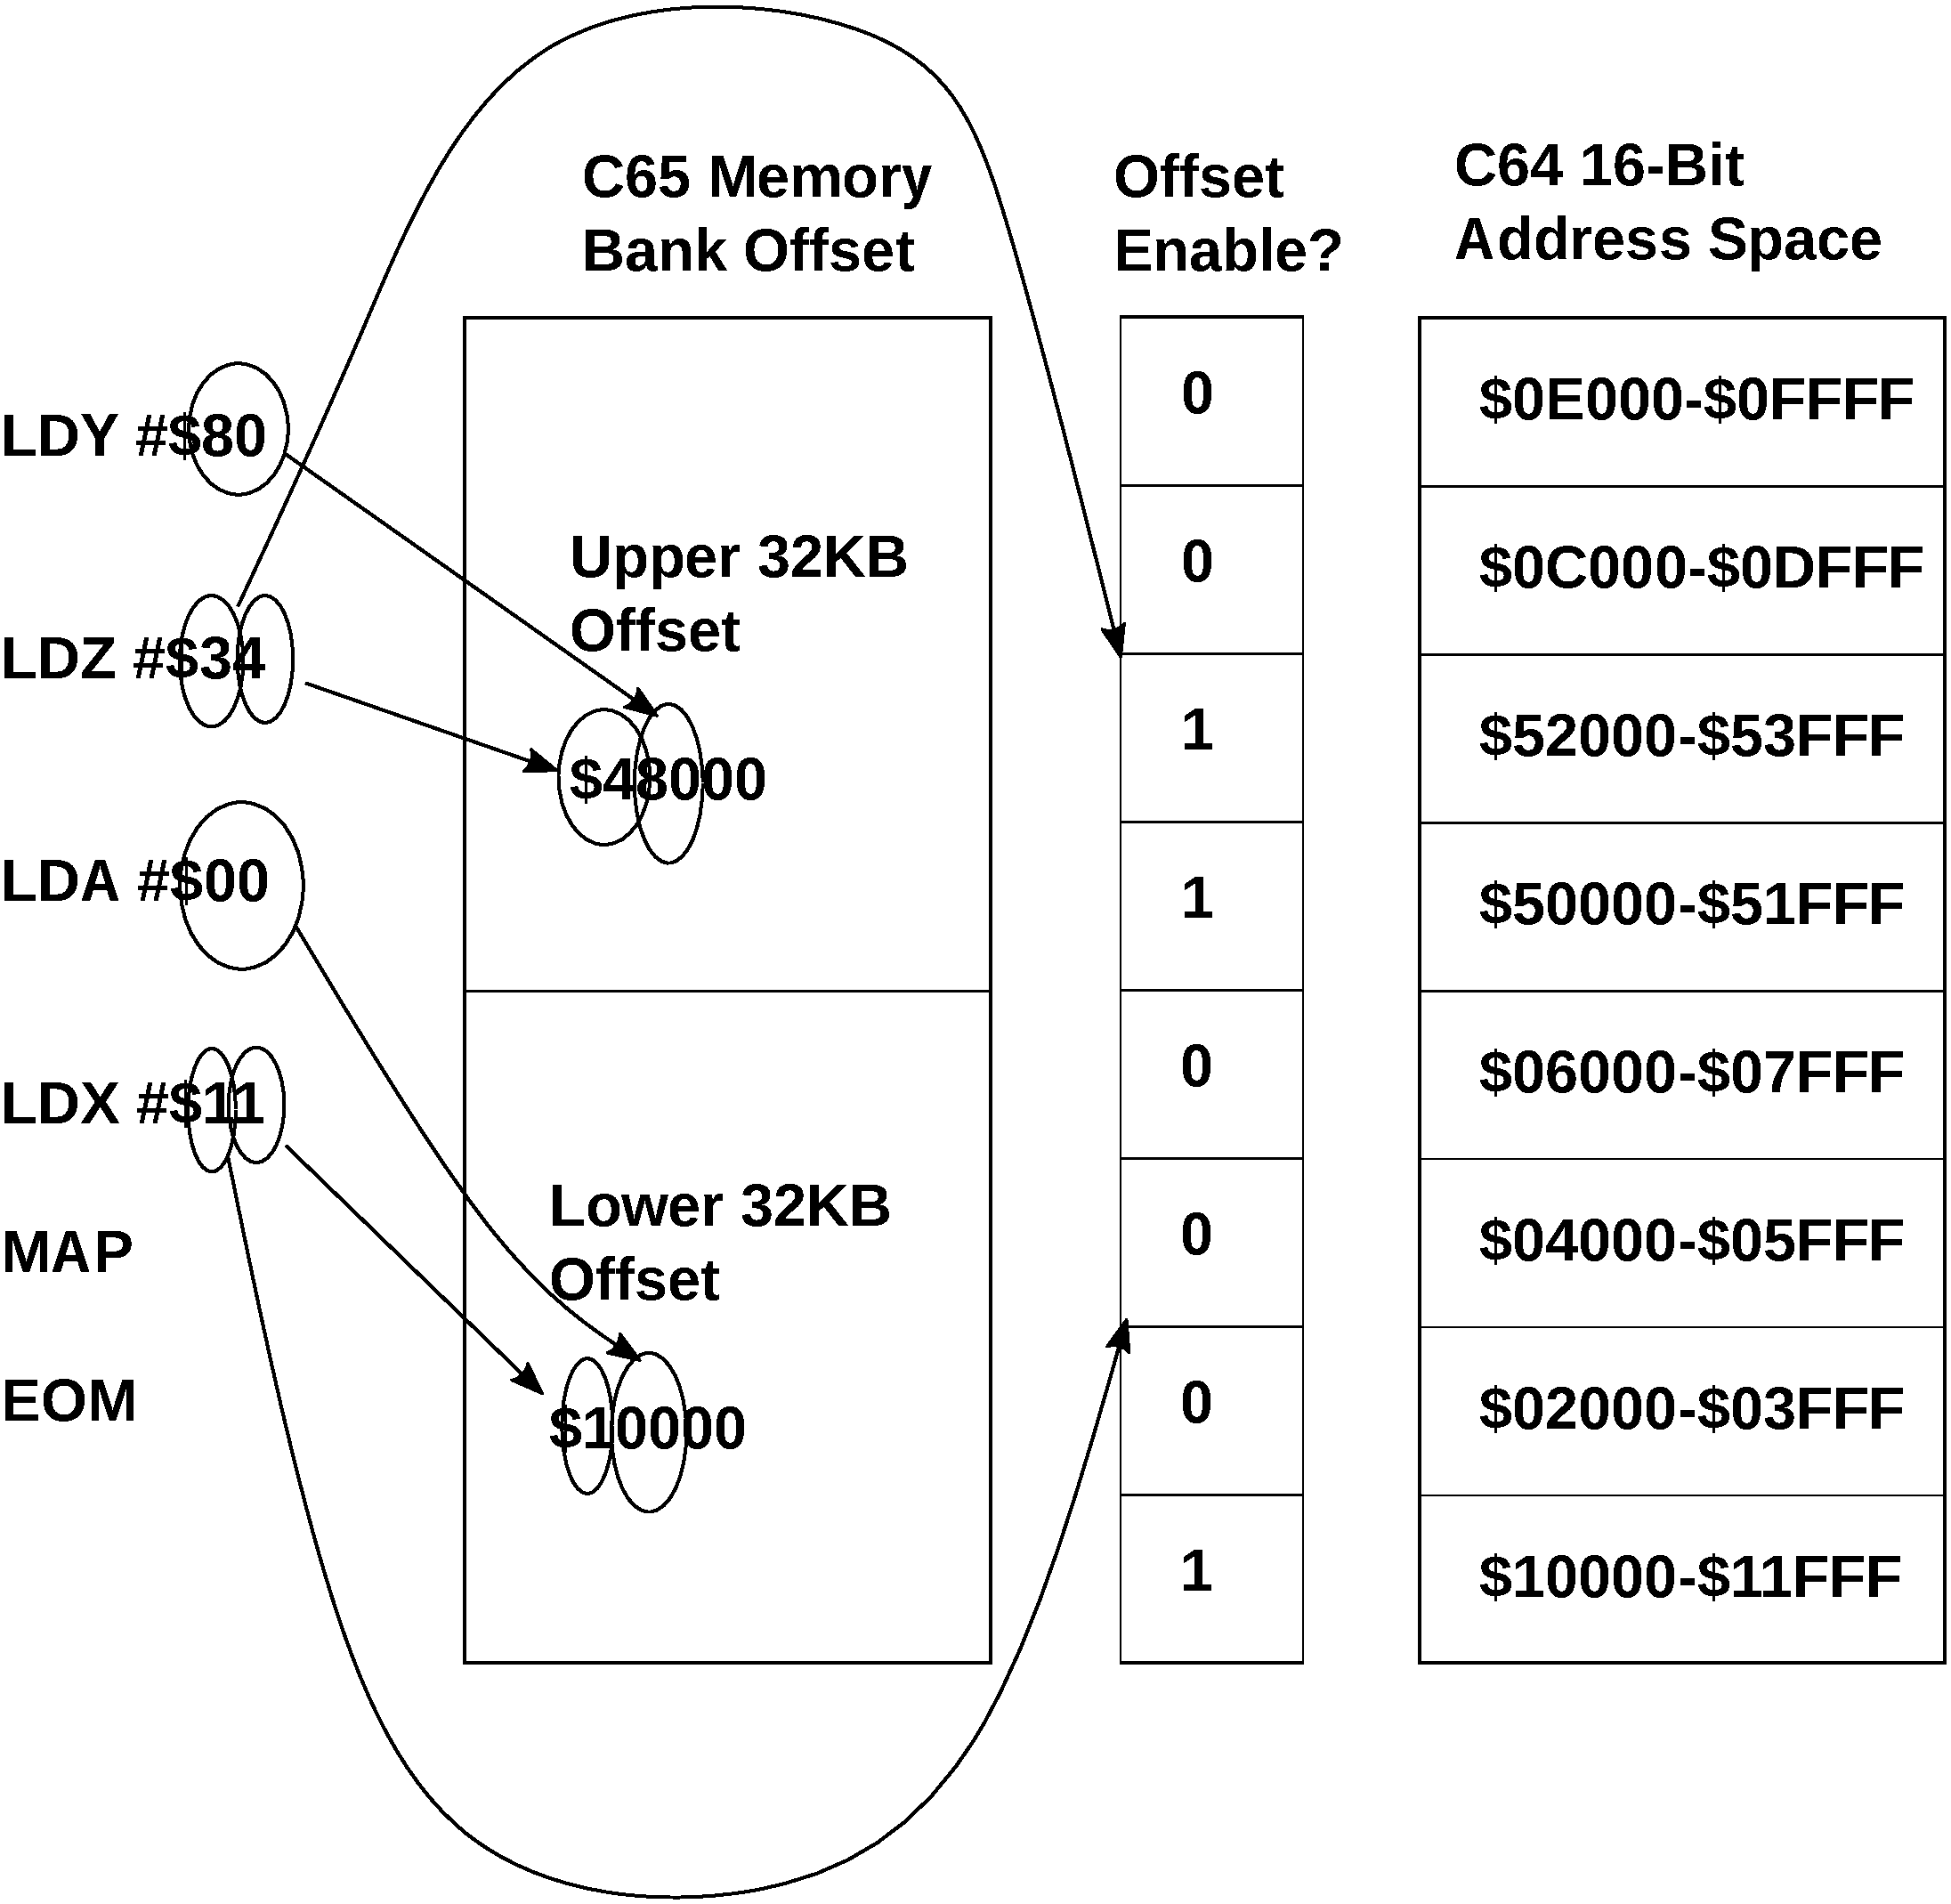
\includegraphics[width=0.75\textwidth]{images/illustrations/map-instruction-operation-example1.pdf}\index{MAP}\index{Memory banking}
\end{center}

Notice that the offsets for each of the two 32KB address ranges get added to the 6502 address.
This is why the offset of \$48000 for the upper 32KB generates an address of \$50000 at the 6502
address \$8000.

See also under ``Using the MAP instruction to access >1MB'' for further explanation.

\subsubsection{Direct Memory Access (DMA) Controller}

The C65's F018/F018A DMA controller allows for rapid filling, copying and swapping of the contents of memory
anywhere in the 1MB address space. Detailed information about the F018 DMA controller, and the MEGA65's
enhancements to this, refer to \bookvref{cha:dmagic}

\subsubsection{Flat Memory Access}

\subsection{Accessing memory beyond the 1MB point}
\label{sec:extended-memory}

The MEGA65 can support up to 256MB of memory. This is more than the 1MB address space of the CSG4510
on which it is based. There are several ways of performing this.

\subsubsection{Using the MAP instruction to access >1MB}

The full address space is available to the MAP instruction for legacy C65-style memory
mapping, although some care is required, as the MAP instruction must be called up to three times.
The reason for this is that the MAP instruction must be called to first select which mega-byte of
memory will be used for the lower and upper map regions, before it is again called in the normal
way to set the memory mapping.  Because between these two calls the memory mapping offset will be
a mix of the old and new addresses, all mapping should be first disabled via the MAP instruction.
This means that the code to re-map memory should live in the bottom 64KB of RAM or in one of the
ROM-bankable regions, so that it can remain visible during the mapping process.

Failure to handle this situation properly will result in the processor executing instructions
from somewhere unexpected half-way through the process, because the routine it is executing
to perform the mapping will suddenly no longer be mapped.

Because of the relative complexity of this process, and the other problems with the MAP instruction
as a means of memory access, we recommend that for accessing data outside of the current memory
map that you use either DMA or the flat-memory address features of the 45GS02 that are described below.
Indeed, access to the full address space via the MAP instruction is only provided for completeness.

As an other example of how the MAP instruction can be used to map an area of memory from
the expanded address space, the following program maps the Ethernet frame buffer from its natural location
at \$FFDE8000 to appear at \$6800.  To keep the example as simple as possible, we assume that the code
is running from in the bottom 64KB of RAM, and not in the region between \$6000 -- \$8000.

As the MAP instruction normally is only aware of the C65-style 20-bit addresses, the MEGA65 extension to the
instruction must be used to set the upper 8 bits of the 28-bit MEGA65 addresses, i.e., which mega-byte of address
space should be used for the address translation.  This is done by setting the X
register to \$0F when setting the mega-byte number for the lower-32KB of the C64-style 64KB address space.
This does not create any incompatibility with any sensible use of the MAP instruction on a C65, because this
value indicates that none of the four 8KB memory blocks will be re-mapped, but at the same time specifies that
the upper 4 bits of the address offset for re-mapped block is the non-zero value of \$F.  The mega-byte number
is then specified by setting the A register.

The same approach applies to the upper 32KB, but using the Z and Y
registers instead of the X and A registers.  However, in this case, we do not need to re-map the upper 32KB of
memory in this example, we will leave the Z and Y registers set to zero.  We must however set X and A to
set the mega-byte number for the lower-32KB to \$FF. Therefore A must have the value \$FF.  To set the lower 20-bits
of the address offset we use the MAP instruction a second time, this time using it in the normal C65 manner.
As we want to remap \$6800 to \$FFDE800, and have already dealt with the \$FFxxxxx offset via the mega-byte number,
we need only to apply the offset to make \$6800 point to \$DE800. \$DE800 minus \$6800 = \$D8000.  As the MAP instruction
operates with a mapping granularity of 256 bytes = \$100, we can drop the last two digits from \$D8000 to obtain the
MAP offset of \$D80. The lower 8-bits, \$80, must be loaded into the A register. The upper 4-bits, \$D, must be loaded into
the low-nibble of the X register.  As we wish to apply the mapping to only the fourth of the 8KB blocks that make up the
lower 32KB half of the C64 memory map, we must set the 4th bit of the upper nibble. That is, the upper nibble must be set
to \%1000, i.e., \$8.  Therefore the X register must be loaded with \$8D.  Thus we yield the complete example program:

\begin{screenoutput}
; Map Ethernet registers at $6000 - $7FFF

; Ethernet controller really lives $FFDE000 - $FFDEFFF, so select $FF megabyte section for MAP LO
LDA #$ff
LDX #$0f
LDY #$00
LDZ #$00
map

; now enable mapping of $DE000-$DFFFF at $6000
; MAPs are offset based, so we need to subtract $6000 from the target address
; $DE000 - $6000 = $D8000
LDA #$80
LDX #$8d
LDY #$00
LDZ #$00
map
EOM

; Ethernet buffer now visible at $6800 - $6FFF
\end{screenoutput}

Note that the EOM (End Of Mapping) instruction (which is the same as NOP on a 6502, i.e., opcode \$EA) was only supplied after the last MAP instruction, to make sure that no interrupts could occur while
the memory map contained mixed values with the mega-byte number set, but the lower-bits of the mapping address had not been
updated.

No example in BASIC for the MAP instruction is possible, because the MAP is an machine code instruction of the 4510 / 45GS02 processors.

\subsubsection{Flat-Memory Access}

The 45GS02 makes it easy to read or write a byte from anywhere in memory by allowing the Zero-Page Indirect
addressing mode to use a 32-bit pointer instead of the normal 16-bit pointer.  This is accomplished by
using the Z-indexed Zero-Page Indirect Addressing Mode for the access, and having the instruction directly
preceded by a NOP instruction (opcode \$EA).  For example:

\begin{screenoutput}
NOP
LDA ($45),Z
\end{screenoutput}

If you are using the ACME assembler, or another assembler that supports the 45GS02 extensions, you can instead use square-brackets
to indicate that you are performing a flat-memory operation. Such assemblers will insert the \$EA prefix automatically for you. For example:

\begin{screenoutput}
LDA [$45],Z
\end{screenoutput}

Regardless which tool you are using, this example would read the four bytes of Zero-Page memory at \$45 -- \$48 to form a 32-bit memory address, and add the value of the
Z register to this to form the actual address that will be read from.  The byte order in the address is the same as
the 6502, i.e., the right-most (least significant) byte of the address will be read from the first address (\$45 in this case),
and so on, until the left-most (most significant) byte will be read from \$48.  For example, to read from memory location
\$12345678, the contents of memory beginning at \$45 should be 78 56 34 12.

This method is much more efficient and also simpler than either using the MAP instruction or the DMA controller for single memory accesses,
and is what we generally recommend.  The DMA controller can be used for moving/filler larger regions of memory.
We recommend the MAP instruction only be used for banking code, or in rare situations where extensive access to a small region of
memory is required, and the extra cycles of reading the 32-bit addresses is problematic.

\subsection{Virtual 32-bit Register}

The 45GS02 allows the use of its four general purpose registers, A, X, Y and Z (A is LSB, Z is MSB) as a single virtual 32-bit register, 
also called the {\em Q pseudo register}.
This can greatly simplify and speed up many common operations, and help avoid many common programming errors.
For example, adding two 16-bit or 32-bit values can now be easily accomplished with something like:

\begin{screenoutput}
  ; Clear carry before performing addition, as normal
  CLC
  ; Prefix an instruction with two NEG instructions to select virtual 32-bit register mode
  NEG
  NEG
  LDA $1234  ; Load the contents of $1234-$1237 into A,X,Y and Z respectively
  ; And again, for the addition
  NEG
  NEG
  ADC $1238  ; Add the contents of $1238-$123B
  ; The result of the addition is now in A, X, Y and Z.
  ; And can be written out in whole or part

  ; To write it all out, again, we need the NEG + NEG prefix
  NEG
  NEG
  STA $123C ; Write the whole out to $123C-$123F

  ; Or to write out the bottom bytes, we can just write the contents of A and X as normal
  STA $1240
  STX $1241
\end{screenoutput}

This approach works with the LDA, STA, ADC, SBC, CMP, EOR, AND, BIT, ORA, ASL, ASR, LSR, ROL, ROR, INC and DEC instructions.
If you are using ACME or another 45GS02 aware assembler, you can instead use the new \stw{LDQ}, \stw{STQ}, \stw{ADCQ},
\stw{SBCQ}, \stw{CPQ}, \stw{EORQ}, \stw{ANDQ}, \stw{BITQ}, \stw{ORQ}, \stw{ASLQ}, \stw{ASRQ}, \stw{LSRQ}, \stw{ROLQ}, \stw{RORQ}, \stw{INQ} and \stw{DEQ}
mnemonics.\index{LDQ}\index{STQ}\index{ADCQ}\index{SBCQ}\index{CPQ}\index{EORQ}\index{ANDQ}\index{BITQ}\index{ORQ}\index{ASLQ}\index{ASRQ}\index{LSRQ}\index{ROLQ}\index{RORQ}\index{INQ}\index{DEQ} The previous example would thus become:

\begin{screenoutput}
  ; Clear carry before performing addition, as normal
  CLC
  LDQ  $1234  ; Load the contents of $1234-$1237 into A,X,Y and Z respectively
  ADCQ $1238  ; Add the contents of $1238-$123B
  ; The result of the addition is now in A, X, Y and Z.
  ; And can be written out in whole or part

  ; To write it all out, again, we need the NEG + NEG prefix
  STQ $123C ; Write the whole out to $123C-$123F

  ; Or to write out the bottom bytes, we can just write the contents of A and X as normal
  STA $1240
  STX $1241
\end{screenoutput}

The virtual 32-bit addressing mode works with any addressing mode.
However, indexed addressing modes, where X, Y or Z are added to the address should
be used with care, because these registers may in fact be holding part of a 32-bit value.

The exception is the Zero-Page Indirect Z-Indexed addressing mode: In this case the Z register is NOT added to the target address
(with the exception of the LDQ opcode), unlike would normally be the case. This is to allow the virtual 32-bit register to be able
to be used with flat-memory access with the combined prefix of \stw{NEG NEG NOP},  before the instruction to allow accessing a
32-bit value anywhere in memory in a single instruction.

Note that the virtual 32-bit register cannot be used in immediate mode, e.g., to load a constant into the four general
purpose registers, or to add or subtract a constant value.  This is to avoid problems with variable length instructions.

For LDQ and STQ, it would save at most one byte
compared to LDA \#\$nn ... LDZ \#\$nn, and would be no faster.  In fact, for many common
values, such as \#\$00000000, there are short-cuts, such as:

\begin{screenoutput}
LDA #$00
TAX
TAY
TAZ
\end{screenoutput}

If you need to add or subtract a 32-bit immediate value, this may require you to re-order the arguments, or perform other
minor gymnastics.  For example, to compute the sum of the contents of memory and an immediate value, you can load the A, X, Y
and Z registers with the immediate value, and then use \stw{ADCQ} with the memory address, e.g.:

\begin{screenoutput}
  ; Get the immediate value #$12345678 into Q
  LDA #$78
  LDX #$56
  LDY #$34
  LDZ #$12
  ; Add the contents of memory locations $1234-$1237
  NEG
  NEG
  ADC $1234
  ; Store the result back in $1234-$1237
  NEG
  NEG
  STA $1234
\end{screenoutput}

Again, if you are using the ACME or another 45GS02-aware assembler, this can be more compactly and
clearly written as follows. But note that in both cases the same byte-sequence of machine code is
produced, and the program will take the same number of cycles to execute.

\begin{screenoutput}
  ; Get the immediate value #$12345678 into Q
  LDA #$78
  LDX #$56
  LDY #$34
  LDZ #$12
  ; Add the contents of memory locations $1234-$1237
  ADCQ $1234
  ; Store the result back in $1234-$1237
  STQ $1234
\end{screenoutput}

\section{C64 CPU Memory Mapped Registers}

\input{regtable_CPU.C64}

\section{New CPU Memory Mapped Registers}

\input{regtable_CPU.MEGA65}

\section{MEGA65 CPU Maths Acceleration Registers}

Every MEGA65 contains a combined 32-bit hardware multiplier and divider.
This device takes two 32-bit inputs, {\bf MULTINA} and {\bf MULTINB}, and simultaneously calculates:

\begin{itemize}
\item the 64-bit product {\bf MULTOUT} of {\bf MULTINA} and {\bf MULTINB}
\item the 32-bit whole part {\bf DIVOUT}(4-7) of {\bf MULTINA} divided by {\bf MULTINB}
\item the 32-bit fractional part {\bf DIVOUT}(0-3) of {\bf MULTINA} divided by {\bf MULTINB}
\end{itemize}

It is always updating the outputs based on the inputs, so there is no need to take special action when changing the inputs.
The multiplier takes 1 cycle to calculate, and the updated result will thus be available immediately (a {\bf MULBUSY} bit is
defined, but currently it won't be set at all). The hardware divider, however, can take upto 20 cycles depending on the
particular inputs. The programmer should check the {\bf DIVBUSY} bit if the divider is still calculating:

\begin{screenoutput}
loop:   BIT $D70F   ; transfer DIVBUSY bit into N flag
        BMI loop    ; as long as it is set, we need to wait
\end{screenoutput}

The MEGA65 is planned to also include a programmable math unit, which helps to accelerate the calculation of fixed-point formulae.
This is presently disabled and will be further documented if and when it becomes available (addresses \$D780 - \$D7E3).

\input{regtable_MATH.MEGA65}

\section{MEGA65 Hypervisor Mode}
\label{sec:hypervisor-mode}

\subsection{Reset}

On power-up or reset, the MEGA65 starts up in hypervisor mode, and expects to find a program in the
16KB hypervisor memory, and begins executing instructions at address \$8100.  Normally a JMP instruction
will be located at this address, that will jump into a reset routine. That is, the 45GS02
does not use the normal 6502 reset vector. It's function is emulated by the Hyppo hypervisor program,
which fetches the address from the 6502 reset vector in the loaded client operating system when
exiting hypervisor mode.

The hypervisor memory is automatically mapped on reset to \$8000 - \$BFFF.  This special memory is not
able to mapped or in anyway accessed, except when in hypervisor mode. It can, however, always be accessed from the serial monitor/debugger
interface via its 28-bit address, \$FFF8000 -- \$FFFBFFF.  This is to protect it from accidental or malicious access from a guest operating system.

\subsection{Entering / Exiting Hypervisor Mode}

Entering the Hypervisor occurs whenever any of the following events occurs:

\begin{itemize}
\item{\bf Power-on} When the MEGA65 is first powered on.
\item{\bf Reset} If the reset line is lowered, or a watch-dog triggered reset occurs.
\item{\bf SYSCALL register accessed} The registers \$D640 - \$D67F in the MEGA65 I/O context trigger SYSCALLs when accessed.
  This is intended to be the mechanism by which a client operating system or process requests the attention of the hypervisor or operating system.
\item{\bf Page Fault} On MEGA65s that feature virtual memory, a page fault will cause a trap to hypervisor mode.
\item{\bf Certain keyboard events} Pressing \widekey{RESTORE} for >0.5 seconds, or the \specialkey{ALT} and
\specialkey{TAB} key combination traps to the hypervisor.  Typically the first is used to launch the Freeze Menu an the second to toggle the display of debug interface.
\item{\bf Accessing virtualised I/O devices} For example, if the F011 (internal 3.5'' disk drive controller) has been virtualised, then attempting to read or write sectors using this device will cause traps to the hypervisor.
  \item{\bf Executing an instruction that would lock up the CPU} A number of undocumented opcodes on the 6502 will cause the CPU to lockup.  On the MEGA65, instead of locking up, the computer will trap to the hypervisor.  This could be used to implement alternative instruction behaviours, or simply to tell the user that something bad has happened.
  \item{\bf Certain special events} Some devices can generate hypervisor-level interrupts. These are implemented as traps to the hypervisor.
\end{itemize}

The 45GS02 handles all of these in a similar manner internally:

\begin{enumerate}
\item The SYSCALL or trap address is calculated, based on the event.
\item The contents of all CPU registers are saved into the virtualisation control registers.
\item The hypervisor mode memory layout is activated, the CPU decimal flag and special purpose registers are all set to appropriate values.  The contents of the A,X,Y and Z and most other CPU flags are preserved, so that they can be accessed from the Hypervisor's SYSCALL/trap handler routine, without having to load them, thus saving a few cycles for each call.
\item The hypervisor-mode flag is asserted, and the program counter (PC) register is set to the computed address.
\end{enumerate}

All of the above happens in one CPU cycle, i.e., in 25 nano-seconds.
Returning from a SYSCALL or trap consists simply of writing to \$D67F, which
requires 125 nano-seconds, for a total overhead of 150 nano-seconds.
This gives the MEGA65 SYSCALL performance rivalling -- even beating
-- even the fastest modern computers, where the system call latency is
typically hundreds to tens of thousands of cycles \cite{soares2010flexsc}.

\subsection{Hypervisor Memory Layout}

The hypervisor memory is 16KB in size.  The first 512 bytes are
reserved for SYSCALL and system trap entry
points, with four bytes for each.  For example, the reset entry point is
at \$8100 - \$8100 + 3 = \$8100 - \$8103.
This allows 4 bytes for an instruction, typically a JMP instruction,
followed by a NOP to pad it to 4 bytes.

The full list of SYSCALLs and traps is:

\begin{longtable}{|L{1.2cm}|L{1.1cm}|C{2cm}|L{6cm}|}
\hline
{\bf{HEX}} & {\bf{DEC}} & {\bf{Name}} & {\bf{Description}} \\
\hline
\endfirsthead
\multicolumn{3}{l@{}}{\ldots continued}\\
\hline
{\bf{HEX}} & {\bf{DEC}} & {\bf{Name}} & {\bf{Description}} \\
\hline
\endhead
\multicolumn{3}{l@{}}{continued \ldots}\\
\endfoot
\hline
\endlastfoot
\small  8000 & \small 32768 & SYSCALL00 & SYSCALL 0 entry point \\
\hline
\small  8004 & \small 32772 & SYSCALL01 & SYSCALL 1 entry point \\
\hline
\small  8008 & \small 32776 & SYSCALL02 & SYSCALL 2 entry point \\
\hline
\small  800C & \small 32780 & SYSCALL03 & SYSCALL 3 entry point \\
\hline
\small  8010 & \small 32784 & SYSCALL04 & SYSCALL 4 entry point \\
\hline
\small  8014 & \small 32788 & SYSCALL05 & SYSCALL 5 entry point \\
\hline
\small  8018 & \small 32792 & SYSCALL06 & SYSCALL 6 entry point \\
\hline
\small  801C & \small 32796 & SYSCALL07 & SYSCALL 7 entry point \\
\hline
\small  8020 & \small 32800 & SYSCALL08 & SYSCALL 8 entry point \\
\hline
\small  8024 & \small 32804 & SYSCALL09 & SYSCALL 9 entry point \\
\hline
\small  8028 & \small 32808 & SYSCALL0A & SYSCALL 10 entry point \\
\hline
\small  802C & \small 32812 & SYSCALL0B & SYSCALL 11 entry point \\
\hline
\small  8030 & \small 32816 & SYSCALL0C & SYSCALL 12 entry point \\
\hline
\small  8034 & \small 32820 & SYSCALL0D & SYSCALL 13 entry point \\
\hline
\small  8038 & \small 32824 & SYSCALL0E & SYSCALL 14 entry point \\
\hline
\small  803C & \small 32828 & SYSCALL0F & SYSCALL 15 entry point \\
\hline
\small  8040 & \small 32832 & SYSCALL10 & SYSCALL 16 entry point \\
\hline
\small  8044 & \small 32836 & SECURENTR & Enter secure container trap entry point \\
\hline
\small  8048 & \small 32840 & SECUREXIT & Leave secure container trap entry point. \\
\hline
\small  804C & \small 32844 & SYSCALL13 & SYSCALL 19 entry point \\
\hline
\small  8050 & \small 32848 & SYSCALL14 & SYSCALL 20 entry point \\
\hline
\small  8054 & \small 32852 & SYSCALL15 & SYSCALL 21 entry point \\
\hline
\small  8058 & \small 32856 & SYSCALL16 & SYSCALL 22 entry point \\
\hline
\small  805C & \small 32860 & SYSCALL17 & SYSCALL 23 entry point \\
\hline
\small  8060 & \small 32864 & SYSCALL18 & SYSCALL 24 entry point \\
\hline
\small  8064 & \small 32868 & SYSCALL19 & SYSCALL 25 entry point \\
\hline
\small  8068 & \small 32872 & SYSCALL1A & SYSCALL 26 entry point \\
\hline
\small  806C & \small 32876 & SYSCALL1B & SYSCALL 27 entry point \\
\hline
\small  8070 & \small 32880 & SYSCALL1C & SYSCALL 28 entry point \\
\hline
\small  8074 & \small 32884 & SYSCALL1D & SYSCALL 29 entry point \\
\hline
\small  8078 & \small 32888 & SYSCALL1E & SYSCALL 30 entry point \\
\hline
\small  807C & \small 32892 & SYSCALL1F & SYSCALL 31 entry point \\
\hline
\small  8080 & \small 32896 & SYSCALL20 & SYSCALL 32 entry point \\
\hline
\small  8084 & \small 32900 & SYSCALL21 & SYSCALL 33 entry point \\
\hline
\small  8088 & \small 32904 & SYSCALL22 & SYSCALL 34 entry point \\
\hline
\small  808C & \small 32908 & SYSCALL23 & SYSCALL 35 entry point \\
\hline
\small  8090 & \small 32912 & SYSCALL24 & SYSCALL 36 entry point \\
\hline
\small  8094 & \small 32916 & SYSCALL25 & SYSCALL 37 entry point \\
\hline
\small  8098 & \small 32920 & SYSCALL26 & SYSCALL 38 entry point \\
\hline
\small  809C & \small 32924 & SYSCALL27 & SYSCALL 39 entry point \\
\hline
\small  80A0 & \small 32928 & SYSCALL28 & SYSCALL 40 entry point \\
\hline
\small  80A4 & \small 32932 & SYSCALL29 & SYSCALL 41 entry point \\
\hline
\small  80A8 & \small 32936 & SYSCALL2A & SYSCALL 42 entry point \\
\hline
\small  80AC & \small 32940 & SYSCALL2B & SYSCALL 43 entry point \\
\hline
\small  80B0 & \small 32944 & SYSCALL2C & SYSCALL 44 entry point \\
\hline
\small  80B4 & \small 32948 & SYSCALL2D & SYSCALL 45 entry point \\
\hline
\small  80B8 & \small 32952 & SYSCALL2E & SYSCALL 46 entry point \\
\hline
\small  80BC & \small 32956 & SYSCALL2F & SYSCALL 47 entry point \\
\hline
\small  80C0 & \small 32960 & SYSCALL30 & SYSCALL 48 entry point \\
\hline
\small  80C4 & \small 32964 & SYSCALL31 & SYSCALL 49 entry point \\
\hline
\small  80C8 & \small 32968 & SYSCALL32 & SYSCALL 50 entry point \\
\hline
\small  80CC & \small 32972 & SYSCALL33 & SYSCALL 51 entry point \\
\hline
\small  80D0 & \small 32976 & SYSCALL34 & SYSCALL 52 entry point \\
\hline
\small  80D4 & \small 32980 & SYSCALL35 & SYSCALL 53 entry point \\
\hline
\small  80D8 & \small 32984 & SYSCALL36 & SYSCALL 54 entry point \\
\hline
\small  80DC & \small 32988 & SYSCALL37 & SYSCALL 55 entry point \\
\hline
\small  80E0 & \small 32992 & SYSCALL38 & SYSCALL 56 entry point \\
\hline
\small  80E4 & \small 32996 & SYSCALL39 & SYSCALL 57 entry point \\
\hline
\small  80E8 & \small 33000 & SYSCALL3A & SYSCALL 58 entry point \\
\hline
\small  80EC & \small 33004 & SYSCALL3B & SYSCALL 59 entry point \\
\hline
\small  80F0 & \small 33008 & SYSCALL3C & SYSCALL 60 entry point \\
\hline
\small  80F4 & \small 33012 & SYSCALL3D & SYSCALL 61 entry point \\
\hline
\small  80F8 & \small 33016 & SYSCALL3E & SYSCALL 62 entry point \\
\hline
\small  80FC & \small 33020 & SYSCALL3F & SYSCALL 63 entry point \\
\hline
\small  8100 & \small 33024 & RESET & Power-on/reset entry point \\
\hline
\small  8104 & \small 33028 & PAGFAULT & Page fault entry point (not currently used) \\
\hline
\small  8108 & \small 33032 & RESTORKEY & Restore-key long press trap entry point \\
\hline
\small  810C & \small 33036 & ALTTABKEY & ALT+TAB trap entry point \\
\hline
\small  8110 & \small 33040 & VF011RD & F011 virtualised disk read trap entry point \\
\hline
\small  8114 & \small 33044 & VF011WR & F011 virtualised disk write trap entry point \\
\hline
\small  8118 & \small 33048 & BREAKPT & CPU break-point encountered \\
\hline
\small  811C -- 81FB & \small 33048 -- 33275 & RESERVED & Reserved traps point entry \\
\hline
\small  81FC & \small 33276 & CPUKIL & KIL instruction in 6502-mode trap entry point \\
\hline
\end{longtable}

The remainder of the 16KB hypervisor memory is available for use by the programmer, but
will typically use the last 512 bytes for the stack and zero-page, giving an overall memory map as follows:

\begin{longtable}{|L{1.2cm}|L{1.1cm}|L{8cm}|}
\hline
{\bf{HEX}} & {\bf{DEC}} & {\bf{Description}} \\
\hline
\endfirsthead
\multicolumn{3}{l@{}}{\ldots continued}\\
\hline
{\bf{HEX}} & {\bf{DEC}} & {\bf{Description}} \\
\hline
\endhead
\multicolumn{3}{l@{}}{continued \ldots}\\
\endfoot
\hline
\endlastfoot
\small  8000 -- 81FF & \small 32768 -- 33279 & SYSCALL and trap entry points \\
\hline
\small  8200 -- BDFF & \small 33280 -- 48639 & Available for hypervisor or operating system program \\
\hline
\small  8E00 -- BEFF & \small 48640 -- 48895 & Processor stack for hypervisor or operating system \\
\hline
\small  8F00 -- BFFF & \small 48896 -- 49151 & Processor zero-page storage for hypervisor or operating system \\
\hline
\end{longtable}

The stack is used for holding the return address of function calls.  The zero-page storage is typically used for holding
variables and other short-term storage, as is customary on the 6502.

\subsection{Hypervisor Virtualisation Control Registers}

\input{regtable_HCPU.MEGA65}

\subsection{Programming for Hypervisor Mode}

The easiest way to write a program for Hypervisor Mode on the MEGA65 is to use KickC, which is a special version of C
made for writing programs for 6502-class processors.  The following example programs are from KickC's supplied examples.
KickC produces very efficient code, and directly supports the MEGA65's
hypervisor mode quite easily through the use of a linker definition file with the following contents:

\begin{screenoutput}
.file [name="%O.bin", type="bin", segments="XMega65Bin"]
.segmentdef XMega65Bin [segments="Syscall, Code, Data, Stack, Zeropage"]
.segmentdef Syscall [start=$8000, max=$81ff]
.segmentdef Code [start=$8200, min=$8200, max=$bdff]
.segmentdef Data [startAfter="Code", min=$8200, max=$bdff]
.segmentdef Stack [min=$be00, max=$beff, fill]
.segmentdef Zeropage [min=$bf00, max=$bfff, fill]
\end{screenoutput}

This file instructs KickC's assembler to create a 16KB file with the 512 byte SYSCALL/trap entry point region at the start,
followed by code and data areas, and then the stack and zero-page areas. It enforces the size and location of these fields, and
will give an error during compilation if anything is too big to fit.

With this file in place, you can then create a KickC source file that provides data structures for the SYSCALL/trap table, e.g.:

\begin{screenoutput}
// XMega65 KERNAL Development Template
// Each function of the KERNAL is a no-args function
// The functions are placed in the SYSCALLS table surrounded by JMP and NOP

import "string"

// Use a linker definition file (put the previous listing into that file)
#pragma link("mega65hyper.ld")

// Some definitions of addresses and special values that this program uses
const char* RASTER = 0xd012;
const char* VIC_MEMORY = 0xd018;
const char* SCREEN = 0x0400;
const char* BGCOL = 0xd021;
const char* COLS = 0xd800;
const char BLACK = 0;
const char WHITE = 1;

// Some text to display
char[] MESSAGE = "hello world!";
\end{screenoutput}

\begin{screenoutput}
void main() {
    // Initialise screen memory, and select correct font
    *VIC_MEMORY = 0x14;
    // Fill the screen with spaces
    memset(SCREEN, ' ', 40*25);
    // Set the colour of every character on the screen to white
    memset(COLS, WHITE, 40*25);
    // Print the "hello world!" message
    char* sc = SCREEN+40;  // Display it one line down on the screen
    char* msg = MESSAGE; // The massage to display
    // A simple copy routine to copy the string
    while(*msg) {
        *sc++ = *msg++;
    }
    // Loop forever showing two white lines as raster bars
    while(true) {
        if(*RASTER==54 || *RASTER==66) {
            *BGCOL = WHITE;
        } else {
            *BGCOL = BLACK;
        }
    }
}

// Here are a couple sample SYSCALL handlers that just display a character on the screen
void syscall1() {
    *(SCREEN+79) = '>';
}

void syscall2() {
    *(SCREEN+78) = '<';
}

// Now we select the SYSCALL segment to hold the SYSCALL/trap entry point table.
#pragma data_seg(Syscall)

// The structure of each entry point is JMP <handler address> + NOP.
// We have a char (xjmp) to hold the opcode for the JMP instruction,
// and then put the address of the SYSCALL/trap handler in the next
// two points as a pointer, and end with the NOP instruction opcode.
\end{screenoutput}

\begin{screenoutput}
struct SysCall {
    char xjmp;         // Holds $4C, the JMP $nnnn opcode
    void()* syscall;   // Holds handler address, will be the target of the JMP
    char xnop;         // Holds $EA, the NOP opcode
};

// To save writing 0x4C and 0xEA all the time, we define them as constants
const char JMP = 0x4c;
const char NOP = 0xea;

// Now we can have a nice table of up to 64 SYSCALL handlers expressed
// in a fairly readable and easy format.
// Each line is an instance of the struct SysCall from above, with the JMP
// opcode value, the address of the handler routine and the NOP opcode value.
export struct SysCall[] SYSCALLS = {
    { JMP, &syscall1, NOP },
    { JMP, &syscall2, NOP }
    };

// In this example we had only two SYSCALLs defined, so rather than having
// another 62 lines, we can just ask KickC to make the TRAP table begin
// at the next multiple of $100, i.e., at $8100.
export align(0x100) struct SysCall[] SYSCALL\_RESET = {
    { JMP, &main, NOP }
};
\end{screenoutput}

If you save the first listing into a file called mega65hyper.ld, and the second
into a file called mega65hyper.kc, you can then compile them using KickC with
a command like:

\begin{screenoutput}
  kickc -a mega65hyper
\end{screenoutput}

It will then produce a file called mega65hyper.bin, which you can then try out
on your MEGA65, or run in the XMega65 emulator with a command like:

\begin{screenoutput}
  xmega65 -kickup mega65hyper.bin
\end{screenoutput}

  \chapter{45GS02 \& 6502 Instruction Sets}

The 45GS02 CPU is able to operate in native mode, where it
is compatible with the CSG 4510, and in 6502 compatibility mode,
where 6502 undocumented instructions, also known as illegal
instructions, are supported for compatibility.

When in 4510 compatibility mode, the 45GS02 also supports a number
of extensions through {\em compound instructions}. These work be prefixing
the desired instruction's opcode with one or more {\em prefix bytes}, which
represent sequences of instructions that should not normally occur.  For example,
two \stw{NEG} instructions in a row acts as a prefix to tell the 45GS02 that the
following instruction will operate on 32 bits of data, instead of the usual 8 bits
of data.  This means that a 45GS02 instruction stream can be readily decoded or disassembled,
without needing to set special instruction length flags, as is the case with the 65816
family of microprocessors. The trade-off is increased execution time, as the 45GS02 must
skip over the prefix-bytes.

The remainder of this chapter introduces the addressing modes, instructions, opcodes and
instruction timing data of the 45GS02, beginning with 6502 compatibility mode, before
moving on to 4510 compatibility mode, and the 45GS02 extensions.

\section{Addressing Modes}

The 45GS02 supports 36 different addressing modes, which are explained below.
Many of these are very similar to one another, being variations of the normal 6502
or 65CE02 addressing modes, except that they accept either
32-bit pointers, operate on 32-bits of data, or both.

\subsection{Implied}

In this mode, there are no operands, as the precise function of the instruction is
implied by the instruction itself.  For example, the \screentext{INX} instruction increments
the X Register.

\subsection{Accumulator}

In this mode, the Accumulator is the operand. This is typically used to shift,
rotate or modify the value of the Accumulator Register in some way.  For example,
\screentext{INC A} increments the value in the Accumulator Register.

\subsection{Q Pseudo Register}

In this mode, the Q Pseudo Register is the operand. This is typically used to shift,
rotate or modify the value of the Q Pseudo Register in some way.  For example,
\screentext{ASL Q} shifts the value in the Q Pseudo Register left one bit.

Remember that the Q Pseudo Register is simply the A, X, Y and Z registers acting together
as a pseudo 32-bit register, where A contains the least significant bits, and Z the
most significant bits.  There are some cases where using a Q mode instruction can be
helpful for operating on the four true registers.

\subsection{Immediate Mode}

In this mode, the argument to the instruction is a value that is used directly.
This is indicated by proceeding the value with a \# character. Most assemblers allow
values to be entered in decimal, or in hexadecimal by preceding the value with a \$ sign,
in binary, by preceding the value with a \% sign.  For example, to set the Accumulator
Register to the value 5, you could use the following:

\begin{tcolorbox}[colback=black,coltext=white]
\verbatimfont{\codefont}
\begin{verbatim}
LDA #5
\end{verbatim}
\end{tcolorbox}

The immediate argument is encoded as a single byte following the instruction.  For the above
case, the instruction stream would contain \$A9, the opcode for LDA immediate mode, followed
by \$05, the immediate operand.

\subsection{Immediate Word Mode}

In this mode, the argument is a 16-bit value that is used directly. There is only one instruction
which uses this addressing mode, \screentext{PHW}.  For example, to push the word \$1234
onto the stack, you could use:

\begin{tcolorbox}[colback=black,coltext=white]
\verbatimfont{\codefont}
\begin{verbatim}
PHW #$1234
\end{verbatim}
\end{tcolorbox}

The low byte of the immediate value follows the opcode of the instruction.  The high byte of the
immediate value then follows that.  For the above example, the instruction stream would thus
be \$F4 \$34 \$12.

\subsection{Base Page (Zero-Page) Mode}

In this mode, the argument is an 8-bit address.  The upper 8-bits of the address are taken from
the Base Page Register.  On 6502 processors, there is no Base Page Register, and instead, the
upper 8-bits are always set to zero -- hence the name of this mode on the 6502: Zero-Page. On
the 45GS02, it is possible to move this ``Zero-Page'' to any page in the processor's 64KB view
of memory by setting the Base Page Register using the \screentext{TAB} instruction. Base Page
Mode allows faster access to a 256 region of memory, and uses less instruction bytes to do so.

The argument is encoded as a single byte that immediately follows the instruction opcode. For
example, \screentext{LDA \$12} would read the value stored in location \$12 in the Base Page,
and put it into the Accumulator Register.  The instruction byte stream for this would be
\$85 \$12.

\subsection{Base Page (Zero-Page) Quad Mode}

In this mode, the argument is an 8-bit address.  The upper 8-bits of the address are taken from
the Base Page Register.  On 6502 processors, there is no Base Page Register, and instead, the
upper 8-bits are always set to zero -- hence the name of this mode on the 6502: Zero-Page. On
the 45GS02, it is possible to move this ``Zero-Page'' to any page in the processor's 64KB view
of memory by setting the Base Page Register using the \screentext{TAB} instruction. Base Page
Mode allows faster access to a 256 region of memory, and uses less instruction bytes to do so.

The argument is encoded as a single byte that immediately follows the instruction opcode. For
example, \screentext{LDQ \$12} would read the value stored in locations \$12 -- \$15 in the Base Page,
and put them into the Q Pseudo Register.  

\subsection{Base Page (Zero-Page) X Indexed Mode}

This mode is identical to Base Page Mode, except that the address is formed by taking the
argument, and adding the value of the X Register to it.  In 6502 mode, the result will always
be in the Base Page, that is, any carry due to the addition from the low byte into the high byte
of the address will be ignored.  The encoding for this addressing mode is identical to Base Page
Mode.

\subsection{Base Page (Zero-Page) Quad X Indexed Mode}

This mode is identical to Base Page Quad Mode, except that the address is formed by taking the
argument, and adding the value of the X Register to it.  In 6502 mode, the result will always
be in the Base Page, that is, any carry due to the addition from the low byte into the high byte
of the address will be ignored.  The encoding for this addressing mode is identical to Base Page Quad
Mode.

\subsection{Base Page (Zero-Page) Y Indexed Mode}

This mode is identical to Base Page Mode, except that the address is formed by taking the
argument, and adding the value of the Y Register to it.  In 6502 mode, the result will always
be in the Base Page, that is, any carry due to the addition from the low byte into the high byte
of the address will be ignored.  The encoding for this addressing mode is identical to Base Page
Mode.

\subsection{Base Page (Zero-Page) Base Y Indexed Mode}

This mode is identical to Base Page Quad Mode, except that the address is formed by taking the
argument, and adding the value of the Y Register to it.  In 6502 mode, the result will always
be in the Base Page, that is, any carry due to the addition from the low byte into the high byte
of the address will be ignored.  The encoding for this addressing mode is identical to Base Page Quad
Mode.

\subsection{Base Page (Zero-Page) Z Indexed Mode}

This mode is identical to Base Page Mode, except that the address is formed by taking the
argument, and adding the value of the Z Register to it.  In 6502 mode, the result will always
be in the Base Page, that is, any carry due to the addition from the low byte into the high byte
of the address will be ignored.  The encoding for this addressing mode is identical to Base Page
Mode.

\subsection{Base Page (Zero-Page) Quad Z Indexed Mode}

This mode is identical to Base Page Quad Mode, except that the address is formed by taking the
argument, and adding the value of the Z Register to it.  In 6502 mode, the result will always
be in the Base Page, that is, any carry due to the addition from the low byte into the high byte
of the address will be ignored.  The encoding for this addressing mode is identical to Base Page Quad
Mode.

\subsection{Absolute Mode}

In this mode, the argument is an 16-bit address.  The low 8-bits of the address are taken from
the byte immediately following the instruction opcode. The upper 8-bits are taken from the
byte following that.  For example, the instruction \screentext{LDA \$1234}, would read the
memory location \$1234, and place the read value into the Accumulator Register.  This would
be encoded as \$AD \$34 \$12.

\subsection{Absolute Quad Mode}

In this mode, the argument is an 16-bit address.  The low 8-bits of the address are taken from
the byte immediately following the instruction opcode. The upper 8-bits are taken from the
byte following that.  For example, the instruction \screentext{LDQ \$1234}, would read the
memory locations \$1234 -- \$1237, and place the read values into the Q Pseudo Register.  This would
be encoded as \$42 \$42 \$AD \$34 \$12.

\subsection{Absolute X Indexed Mode}

This mode is identical to Absolute Mode, except that the address is formed by taking the
argument, and adding the value of the X Register to it.  If the indexing causes the address
to cross a page boundary, i.e., if the upper byte of the address changes, this may incur a
1 cycle penalty, depending on the processor mode and speed setting.
The encoding for this addressing mode is identical to Absolute Mode.

\subsection{Absolute Quad X Indexed Mode}

This mode is identical to Absolute Quad Mode, except that the address is formed by taking the
argument, and adding the value of the X Register to it.  If the indexing causes the address
to cross a page boundary, i.e., if the upper byte of the address changes, this may incur a
1 cycle penalty, depending on the processor mode and speed setting.
The encoding for this addressing mode is identical to Absolute Quad Mode.

\subsection{Absolute Y Indexed Mode}

This mode is identical to Absolute Mode, except that the address is formed by taking the
argument, and adding the value of the Y Register to it.  If the indexing causes the address
to cross a page boundary, i.e., if the upper byte of the address changes, this may incur a
1 cycle penalty, depending on the processor mode and speed setting.
The encoding for this addressing mode is identical to Absolute Mode.

\subsection{Absolute Quad Y Indexed Mode}

This mode is identical to Absolute Quad Mode, except that the address is formed by taking the
argument, and adding the value of the Y Register to it.  If the indexing causes the address
to cross a page boundary, i.e., if the upper byte of the address changes, this may incur a
1 cycle penalty, depending on the processor mode and speed setting.
The encoding for this addressing mode is identical to Absolute Quad Mode.

\subsection{Absolute Z Indexed Mode}

This mode is identical to Absolute Mode, except that the address is formed by taking the
argument, and adding the value of the Z Register to it.  If the indexing causes the address
to cross a page boundary, i.e., if the upper byte of the address changes, this may incur a
1 cycle penalty, depending on the processor mode and speed setting.
The encoding for this addressing mode is identical to Absolute Mode.

\subsection{Absolute Quad Z Indexed Mode}

This mode is identical to Absolute Quad Mode, except that the address is formed by taking the
argument, and adding the value of the Z Register to it.  If the indexing causes the address
to cross a page boundary, i.e., if the upper byte of the address changes, this may incur a
1 cycle penalty, depending on the processor mode and speed setting.
The encoding for this addressing mode is identical to Absolute Quad Mode.

\subsection{Absolute Indirect Mode}

In this mode, the 16-bit argument is the address that points to, i.e., contains the
address of actual byte to read.  For example, if memory location \$1234 contains \$78
and memory location \$1235 contains \$56, then \screentext{JMP (\$1234)} would jump
to address \$5678.  The encoding for this addressing mode is identical to Absolute Mode.

\subsection{Absolute Indirect X-Indexed Mode}

In this mode, the 16-bit argument is the address that points to, i.e., contains the
address of actual byte to read. It is identical to Absolute Indirect Mode, except that
 the value of the X Register is added to the pointer address.
For example, if the X Register contains the value \$04, memory location \$1238 contains \$78
and memory location \$1239 contains \$56, then \screentext{JMP (\$1234)} would jump
to address \$5678.
The encoding for this addressing mode is identical to Absolute Mode.

\subsection{Base Page Indirect X-Indexed Mode}

This addressing mode is identical to Absolute Indirect X-Indexed Mode, except that the address
of the pointer is formed from the Base Page Register (high byte) and the 8-bit operand (low byte).
The encoding for this addressing mode is identical to Base Page Mode.

\subsection{Base Page Quad Indirect X-Indexed Mode}

This addressing mode is identical to Base PAge Indirect X-Indexed Mode, except that the address
of the pointer is formed from the Base Page Register (high byte) and the 8-bit operand (low byte).
The encoding for this addressing mode is identical to Base Page Quad Mode.

\subsection{Base Page Indirect Y-Indexed Mode}

This addressing mode differs from the X-Indexed Indirect modes, in that the Y Register is
added to the address that is read from the pointer, instead of being added to the pointer.
This is a very useful mode, that is frequently because it effectively provides access to
``the Y-th byte of the memory at the address pointed to by the operand.'' That is, it de-references
a pointer.
The encoding for this addressing mode is identical to Base Page Mode.

\subsection{Base Page Quad Indirect Y-Indexed Mode}

This addressing mode is identical to the Base Page Indirect Y-Indexed Mode, except that
32-bits of data are operated on. The encoding for this addressing mode is identical to
Base Page Mode, except that it is prefixed by \$42, \$42.

\subsection{Base Page Indirect Z-Indexed Mode}

This addressing mode differs from the X-Indexed Indirect modes, in that the Z Register is
added to the address that is read from the pointer, instead of being added to the pointer.
This is a very useful mode, that is frequently because it effectively provides access to
``the Z-th byte of the memory at the address pointed to by the operand.'' That is, it de-references
a pointer.
The encoding for this addressing mode is identical to Base Page Mode.

That is, it is equivalent to the Base Page Indirect Y-Indexed Mode.

\subsection{Base Page Quad Indirect Z-Indexed Mode}

This addressing mode is identical to the Base Page Indirect Z-Indexed Mode, except that
32-bits of data are operated on. The encoding for this addressing mode is identical to
Base Page Mode, except that it is prefixed by \$42, \$42.

\subsection{32-bit Base Page Indirect Z-Indexed Mode}

This mode is formed by preceding a Base Page Indirect Z-Indexed Mode instruction with
the {NOP} instruction (opcode \$EA).  This causes the 45GS02 to read a 32-bit address instead
of a 16-bit address from the Base Page address indicated by its operand.  The Z index is added
to that pointer.  Importantly, the 32-bit address does not refer to the processor's current 64KB
view of memory, but rather to the 45GS02's true 28-bit address space. This allows easy access
to any memory, without requiring the use of complex bank-switching or DMA operations.

For example, if addresses \$12 to \$15 contained the bytes \$20, \$D0, \$FF, \$0D, and the
Z index contained the value \$01, the following instruction sequence would change the screen
colour to blue:

\begin{tcolorbox}[colback=black,coltext=white]
\verbatimfont{\codefont}
\begin{verbatim}
LDA #$06
LDZ #$01
STA [$12],Z
\end{verbatim}
\end{tcolorbox}

\subsection{32-bit Base Page Indirect Quad Z-Indexed Mode}

This addressing mode is identical to the 32-bit Base Page Indirect Z-Indexed Mode,
except that it operates on 32-bits of data at the 32-bit address formed by the argument,
in comparison to 32-bit Base Page Indirect Z-Indexed Mode which operates on only 8 bits
of data.   The encoding of this addressing mode is \$42, \$42, \$EA, followed by the
natural 6502 opcode for the instruction being performed.


\subsection{32-bit Base Page Indirect Mode}

This mode is formed by preceding a Base Page Indirect Z-Indexed Mode instruction with
the {NOP} instruction (opcode \$EA).  This causes the 45GS02 to read a 32-bit address instead
of a 16-bit address from the Base Page address indicated by its operand.
Importantly, the 32-bit address does not refer to the processor's current 64KB
view of memory, but rather to the 45GS02's true 28-bit address space. This allows easy access
to any memory, without requiring the use of complex bank-switching or DMA operations.

For example, if addresses \$12 to \$15 contained the bytes \$20, \$D0, \$FF, \$0D,
the following instruction sequence would change the screen border colour to blue:

\begin{tcolorbox}[colback=black,coltext=white]
\verbatimfont{\codefont}
\begin{verbatim}
LDA #$06
STA [$12]
\end{verbatim}
\end{tcolorbox}

NOTE: The ACME assembler is the only assembler that currently supports this addressing mode.
For other assemblers, you can achieve the same result by using a \stw{NOP} instruction to
prefix the equivalent {\em Base Page Indirect, Indexed by Z} instruction.

\begin{tcolorbox}[colback=black,coltext=white]
\verbatimfont{\codefont}
\begin{verbatim}
LDA #$06
NOP
STA ($12),Z
\end{verbatim}
\end{tcolorbox}


The encoding for this addressing mode is identical to Base Page Mode.

\subsection{32-bit Base Page Indirect Mode}

This addressing mode is identical to the 32-bit Base Page Indirect Mode,
except that it operates on 32-bits of data at the 32-bit address formed by the argument,
in comparison to 32-bit Base Page Indirect Mode which operates on only 8 bits
of data.   The encoding of this addressing mode is \$42, \$42, \$EA, followed by the
natural 6502 opcode for the instruction being performed.

\subsection{Stack Relative Indirect, Indexed by Y}

This addressing mode is similar to Base Page Indirect Y-Indexed Mode,
except that instead of providing the address of the pointer in the
Base Page, the operand indicates the offset in the stack to find the
pointer. This addressing mode effectively de-references a pointer that
has been placed on the stack, e.g., as part of a function call from a
high-level language.  It is encoded identically to the Base Page Mode.

\subsection{Relative Addressing Mode}

In this addressing mode, the operand is an 8-bit signed offset to the
current value of the Program Counter (PC). It is used to allow branches
to encode the near-by address at which execution should proceed if the
branch is taken.

\subsection{Relative Word Addressing Mode}

This addressing mode is identical to Relative Addressing Mode, except that
the address offset is a 16-bit value. This allows a relative branch or jump
to any location in the current 64KB memory view.  This makes it possible
to write software that is fully relocatable, by avoiding the need for absolute
addresses when calling routines.

\section{6502 Instruction Set}

NOTE: The mechanisms for switching from 4510 to 6502 CPU personality
have yet to be finalised.

NOTE: Not all 6502 illegal opcodes are currently implemented.

\subsection{Opcode Map}

\begin{center}
\rotatebox{270}{
\input{6502-opcodes}
}
\end{center}

\subsection{Instruction Timing}

The following table summarises the base instruction timing for 6502 mode.
Please also read the information for 4510 mode, as it discusses a number
of important factors that affect these figures.

\begin{center}
\rotatebox{270}{
\input{6502-cycles}
}
\end{center}

\subsection{Addressing Mode Table}

\begin{center}
  \rotatebox{270}{
    \scriptsize
\input{6502-modes}
}
\end{center}

\subsection{Official And Unintended Instructions}

The 6502 opcode matrix has a size of 16 x 16 = 256 possible opcodes.
Those, that are officially documented, form the set of the
\textcolor{blue}{legal} instructions.
All instructions of this legal set are headed by a blue coloured mnemonic.

The remaining opcodes form the set of the
\textcolor{red}{unintended} instructions
(sometimes called "illegal" instructions).
For the sake of completeness these are documented too.
All instructions of the unintended set are headed by a red coloured mnemonic.

The unintended instructions are implemented in the 6502 mode,
but are not guaranteed to produce exactly the same results as on other
CPU's of the 65xx family. Many of these instructions are known to
be unstable, even running on old hardware.

\input{instructionset-6502}


\section{4510 Instruction Set}

\subsection{Opcode Map}

\begin{center}
\rotatebox{270}{
  \input{4510-opcodes}
  }
\end{center}

\subsection{Instruction Timing}

The following table lists the base cycle count for each opcode.
Note that the number of cycles depends on the speed setting of the
processor: Some instructions take more or fewer cycles when the
processor is running at full-speed, or a C65 compatibility 3.5MHz speed,
or at C64 compatibility 1MHz/2MHz speed.  More detailed information on
this is listed under each each instruction's information, but the high-level
view is:

\begin{itemize}
\item When the processor is running at 1MHz, all instructions take at least
  two cycles, and dummy cycles are re-inserted into Read-Modify-Write instructions,
  so that all instructions take exactly the same number of cycles as on a 6502.
\item The Read-Modify-Write instructions and all instructions that read a value from
  memory all require an extra cycle when operating at full speed, to allow signals
  to propagate within the processor.
\item The Read-Modify-Write instructions require an additional cycle if the operand
  is \$D019, as the dummy write is performed in this case.
  This is to improve compatibility with C64 software that frequently uses this
  ``bug'' of the 6502 to more rapidly acknowledge VIC-II interrupts.
\item Page-crossing and branch-taking penalties do not apply when the processor is
  running at full speed.
\item Many instructions require fewer cycles when the processor is running at full
  speed, as generally most non-bus cycles are removed. For example, Pushing and Pulling
  values to and from the stack requires only 2 cycles, instead of the 4 that that the
  6502 requires for these instructions.
\end{itemize}

Note that it is possible that further changes to processor timing will occur.

Similar issues apply to when the processor is in 6502 mode.

\begin{center}
\rotatebox{270}{
\input{4510-cycles}
}
\end{center}

\subsection{Addressing Mode Table}

\begin{center}
  \rotatebox{270}{
    \scriptsize
\input{4510-modes}
}
\end{center}


\input{instructionset-4510}

\section{45GS02 Compound Instructions}

As the 4510 has no unallocated opcodes, the 45GS02 uses compound instructions
to implement its extension.  These compound instructions consist of one or
more single-byte instructions placed immediately before a conventional
instruction.  These prefixes instruct the 45GS02 to treat the following instruction
differently, as described in \bookvref{cha:cpu}.

% Opcodes can have multiple meanings, so no table

% No instruction timing table for compounds, as it can't
% be correctly drawn.

% Same goes for mode list.


\input{instructionset-45GS02}


  \chapter{F018-Compatible Direct Memory Access (DMA) Controller}
\label{cha:dmagic}

The MEGA65 includes an F018/F018A backward-compatible DMA controller.
Unlike in the C65, where the DMA controller exists as a separate
chip, it is part of the 45GS02 processor in the MEGA65.  However, as the
use of the DMA controller is a logically separate topic, it is documented
separately in this appendix.
 
The MEGA65's DMA controller provides several important improvements over the
F018/F018A DMAgic chips of the C65:
 
\begin{itemize}
\item{\bf Speed} The MEGA65 performs DMA operations at 40MHz, allowing filling 40MiB or copying 20MiB
  per second.  For example, it is possible to copy a complete 8KiB C64-style bitmap display in
  about 200 micro-seconds, equivalent to less than four raster lines!
 \item{\bf Large Memory Access} The MEGA65's DMA controller allows access to all 256MiB of address space.
\item{\bf Texture Copying Support} The MEGA65's DMA controller can do fractional address calculations
  to support hardware texture scaling, as well as address striding, to make it possible in principle
  to simultaneously scale-and-draw a texture from memory to the screen. This would be useful, should
  anyone be crazy enough to try to implement a Wolfenstein or Doom style-game on the MEGA65.
\item{\bf Transparency/Mask Value Support} The MEGA65's DMA controller can be told to ignore a special value
   when copying memory, leaving the destination memory contents unchanged. This allows masking of transparent
   regions when performing a DMA copy, which considerably simplifies blitting of graphics shapes.
\item{\bf Per-Job Option List} A number of options can be configured for each job in a chained list of DMA
  jobs, for example, selecting F018 or F018B mode, changing the transparency value, fractional address stepping
  or the source or destination memory region.

\item{\bf Background Audio DMA}
  The MEGA65 includes background audio DMA capabilities similar to the Amiga\texttrademark series of computers.
  Key differences are that the MEGA65 can use either 8 or 16 bit samples, supports very high sample rates
  up to approximately 1 MHz, has 256 volume settings per channel, and no inter-channel modulation.

\end{itemize}

\section{Audio DMA}

The MEGA65 includes four channels of DMA-driven audio playback that can be used in place of the direct digital
audio registers at \$D6F8-\$D6FB.  That is, you must select which of these two sources to feed to the audio
cross-bar mixer.  This is selected via the AUDEN signal (\$D711 bit 7), which simultaneously enables the audio DMA
function in the processor, as well as instructing the audio cross-bar mixer to use the audio from this instead
of the \$D6F8-\$D6FB digital audio registers. If you wish to have no
other audio than the audio DMA channels, the audio cross-bar mixer can
be bypassed, and the DMA audio played at full volume by setting the
NOMIX signal (\$D711 bit 4).  In that mode no audio from the SIDs, FM,
microphones or other sources will be available.
All other bits in
\$D711 should ordinarily be left clear, i.e., write \$80 to \$D711 to
enable audio DMA.

Two channels form the left digital audio channel, and the other two
channels form the right digital audio channel. It is these left and
right channels that are then fed into the MEGA65's audio cross-bar
mixer.   

As the DMA controller is part of the processor of the MEGA65, and the MEGA65 does not have reserved bus slots
  for multi-media operations, the MEGA65 uses idle CPU cycles to perform background DMA. This requires that the
  MEGA65 CPU be set to the ``full speed'' mode, i.e., approximately 40MHz.  In this mode, there is a wait-state
  whenever reading an operand from memory.  Thus each instruction that loads a byte from memory will create one
  implicit audio DMA slot.  This is rarely a problem in practice, except if the processor idles in a very tight
  loop.  To ensure that audio continues to play in the background, such loops should include a read instruction,
  such as:

\begin{screenoutput}
loop:   LDA $1234   // Ensure loop has at least one idle cycle for
                    // audio DMA
        JMP loop
\end{screenoutput}

Each of the four DMA channels is configured using a block of 16
registers at \$D720, \$D730, \$D740 and \$D750, respectively.
We will explain the registers for the first channel, channel 0, at
\$D720 -- \$D72F.

\subsection{Sample Address Management}

To play an audio sample you must first supply the start address of the
sample. This is a 24-bit address, and must be in the main chip memory
of the MEGA65. This is done by writing the address into \$D72A --
\$D72C.  This is the address of the first sample value that will be played.
You must then provide the end address of the sample in \$D727 --
\$D728.  But note that this is is only 16 bits. This is because the
MEGA65 compares only the bottom 16 bits of the address when checking
if it has reached the end of a sample.  In practice, this means that
samples cannot be more than 64KB in size.  If the sample contains a
section that should be repeated, then the start address of the
repeating part should be loaded into \$D721 -- \$D723, and the CH0LOOP
bit should be set (\$D720 bit 6).  

You can determine the current sample address at any time by reading
the registers at \$D72A -- \$D72C. But beware: These registers are not
latched, so it is possible that the values may be updated as you read
the registers, unless you stop the channel first by clearing the CH0EN
signal.

\subsection{Sample Playback frequency and Volume}

The MEGA65 controls the playback rate of audio DMA samples by using a
24-bit counter.  Whenever the 24-bit counter overflows, the next
sample is requested. Sample speed control is achieved by setting the
value added to this counter each CPU cycle.  Thus a value of
\$FFFFFF would result in a sample rate of almost 40.5 MHz.  In
practice, sample rates above a few megahertz are not possible, because
there are insufficient idle CPU cycles, and distorted audio will
result.  Even below this, care must be taken to ensure that idle
cycles come sufficiently often and dispersed throughout the
processor's instruction stream to prevent distortion.  At typical
sample rates below 16KHz and using 8 bit samples these effects are
typically negligible for normal instruction streams, and so no special
action is normally required for typical audio playback.

At the other end of the scale, sample rates as low as 40.5MHz/$2^{24}$
= 2.4 samples per second are possible.  This is sufficiently low
enough for even the most demanding infra-sound applications.

Volume is controlled by setting \$D629.  Maximum volume is obtained
with the value \$FF, while a value of \$00 will effectively mute the
channel.  The first two audio channels are normally allocated to the
left, and the second two to the right.  However, the MEGA65 includes
separate volume controls for the opposite channels. For example, to
play audio DMA channel 0 at full volume on both left and right sides
of the audio output, set both \$D729 and \$D71C to \$FF.  This allows
panning of the four audio DMA channels.

Both the frequency and volume can be freely adjusted while a sample is playing
to produce various effects.

\subsection{Pure Sine Wave}

Where it is necessary to produce a stable sine wave, especially at
higher frequencies, 
there is a special mode to support this. By setting the CH0SINE
signal, the audio channel will play a 32-byte 16-bit sine wave
pattern.  The sample addresses still need to be set, as though the
sine wave table were located in the bottom 64 bytes of memory, as the
normal address generation logic is used in this mode. However, no
audio DMA fetches are performed when a channel is in this mode, thus
avoiding all sources of distortion due to irregular spacing of idle
cycles in the processor's instruction stream.

This can be used to produce sine waves in both the audible range, as
well as well into the ultrasonic range, at frequencies exceeding
60,000Hz, provided that the MEGA65 is connected to an appropriately
speaker arrangement. 

\subsection{Sample playback control}

To begin a channel playing a sample, set the CH0EN signal (\$D720 bit
7). The sample will play until its completion, unless the CH0LOOP
signal has also been set. When a sample completes playing, the CH0STP
flag will be set.  The audio DMA subsystem cannot presently generate
interrupts.

Unlike on the Amiga\texttrademark, the MEGA65 audio DMA system supports both
8 and 16-bit samples.  It also supports packed 4-bit samples, playing
either the lower or upper nybl of each sample byte.  This allows two
separate samples to occupy the same byte, thus effectively halving the
amount of space required to store two equal length samples.

\section{MEGA65 Enhanced DMA Jobs}

The MEGA65's implementation of the DMAgic supports significantly
enhanced DMA jobs.  An enhanced DMA job is indicated by writing the
low-byte of the DMA list address to \$D705 instead of to \$D700.  The
MEGA65 will then look for one or more {\em job option tokens} at the
start of the DMA list.  Those tokens will be interpretted, before
executing the DMA job which immediately follows the {\em end of job
  options} token (\$00).  Job option tokens which take an argument have the
most-significant bit set, and always take a 1 byte option.  Job option
tokens that take no argument have the most-significant-bit clear.
Unsupported job option tokens are simply ignored.
This allows for future revisions of the DMAgic to add support for
additional options, without breaking backward compatibility.

The list of valid job option tokens is:

\begin{tabular}{|c|l|}
  \hline
  \$00 & End of job option list \\
  \$06 & Enable use of transparent value \\
  \$07 & Disable use of transparent value \\
  \$0A & Use 11-byte F011A DMA list format \\
  \$0B & Use 12-byte F011B DMA list format \\
  \$80 & Source address bits 20 -- 27 \\
  \$81 & Destination address bits 20 -- 27 \\
  \$82 & Source skip rate (256\textsuperscript{ths} of bytes) \\
  \$83 & Source skip rate (whole bytes) \\
  \$84 & Destination skip rate (256\textsuperscript{ths} of bytes) \\
  \$85 & Destination skip rate (whole bytes) \\
  \$86 & Transparent value (bytes with matching value are not written) \\
\end{tabular}




\section{F018 ``DMAgic'' DMA Controller}

\input{regtable_DMA.C65}

\section{MEGA65 DMA Controller Extensions}

\input{regtable_DMA.MEGA65}

\section{Unimplemented Functionality}

The MEGA65's DMAgic does not currently support either memory-swap or
mini-term operations.

Miniterms were intended for bitplane blitting,
which is not required for the MEGA65 which offers greatly advanced
character modes and stepped and fractional DMA address incrementing
which allows efficient texture copying and scaling. Also there exists
no known software which ever used this facility, and it remains
uncertain if it was ever implemented in any revision of the DMAgic
chip used in C65 prototypes. 

The memory-swap
operation is intended to be implemented, but can be worked around in
the meantime by copying the first region to a 3rd region that acts as
a temporary buffer, then copying the 2nd region to the 1st, and the
3rd to the 2nd.

  \chapter{VIC-IV Video Interface Controller}
\label{cha:viciv}

\section{Features}
The VIC-IV is a fourth generation Video Interface Controller developed
especially for the MEGA65, and featuring very good backwards compatibility
with the VIC-II that was used in the C64, and the VIC-III that
was used in the C65.  The VIC-IV can be programmed as though it were either
of those predecessor systems.  In addition it supports a number of new
features. It is easy to mix older VIC-II/III features with the new VIC-IV
features, making it easy to transition from the VIC-II or VIC-III to the VIC-IV,
just as the VIC-III made it easy to transition from the VIC-II.  Some of the new
features and enhancements of the VIC-IV include:

\begin{itemize}
\item {\bf Direct access to 384KB RAM} (up from 16KB/64KB with the VIC-II and 128KB
  with the VIC-IV).
\item Support for {\bf 32KB of 8-bit Colour/Attribute RAM} (up from 2KB on the VIC-III), to
  support very large screens.
\item {\bf HDTV 720$\times$576 / 800$\times$600 native resolution} at both 50Hz and 60Hz for {\bf PAL and NTSC}, with {\bf VGA and digital video} output.
\item {\bf 81MHz pixel clock} (up from $\sim$ 8MHz with the VIC-II/III), which enables a wide range of new features.
\item New 16-colour (16$\times$8 pixels per character cell) and 256-colour (8$\times$8 pixels per character cell) {\bf full-colour text modes}.
\item Support for up to {\bf 8,192 unique characters in a character set}.
\item {\bf Four 256-colour palette banks} (versus the VIC-III's single palette bank), each supporting {\bf 23-bit colour depth} (versus the VIC-III's 12-bit colour depth), and which can be rapidly alternated to create even more colourful graphics than is possible with the VIC-III.
\item Screen, bitmap, colour and character data can be positioned at any {\bf address with byte-level granularity} (compared with fixed 1KB -- 16KB boundaries with the VIC-II/III)
\item {\bf Virtual screen dimensioning}, which combined with byte-level data position granularity provides effective {\bf hardware support for scrolling and panning in both X and Y directions}.
\item {\bf New sprite modes}: Bitplane modification, {\bf full-colour} (15 foreground colours + transparency) and tiled modes, allowing a wide variety of new and exciting sprite-based effects
  \item The ability to stack sprites in a bit-planar manner to produce {\bf sprites with up to 256 colours}.
\item Sprites can use 64 bits of data per raster line, allowing {\bf sprites to be 64 pixels wide} when using VIC-II/III mono/multi-colour mode, or 16 pixels wide when using the new VIC-IV full-colour sprite mode.
\item {\bf Sprite tile mode}, which allows a sprite to be repeated horizontally across an entire raster line, allowing sprites to be used to create  animated backgrounds in a memory-efficient manner.
  \item Sprites can be configured to use a {\bf separate 256-colour palette} to that used to draw other text and graphics, allowing for a more colourful display.
  \item {\bf Super-extended attribute mode} which uses two screen RAM bytes and two colour RAM bytes per character mode, which supports a wide variety of new features including {\bf alpha-blending/anti-aliasing}, {\bf hardware kerning/variable-width characters}, hardware horizontal/vertical flipping, alternate palette selection and other powerful features that make it easy to create highly dynamic and colourful displays.
  \item {\bf Raster-Rewrite Buffer} which allows {\bf hardware-generated pseudo-sprites}, similar to ``bobs'' on Amiga\texttrademark \ computers, but with the advantage that they are rendered in the display pipeline, and thus do not need to be un-drawn and redrawn to animate them.
    \item {\bf Multiple 8-bit colour play-fields} are also possible using the Raster-Rewrite Buffer.

      In short, the VIC-IV is a powerful evolution of the VIC-II/III, while retaining the character and distinctiveness of the VIC-series of
      video controllers.

      For a full description of the additional registers that the VIC-IV provides, as well as documentation of the legacy VIC-II and VIC-III registers, refer to the corresponding sections of this appendix. The remainder of the appendix will focus on describing the capabilities and use of many of the VIC-IV's new features.
\end{itemize}

\section{VIC-II/III/IV Register Access Control}
Because the new features of the VIC-IV are all extensions to the existing VIC-II/III designs, there is no concept of having to select the mode in which the VIC-IV will operate: It is always in VIC-IV mode. However, for backwards compatibility with software, the many additional registers of the VIC-IV can be hidden, so that it appears to be either a VIC-II or VIC-III. This is done in the same manner that the VIC-III uses to hide its new features from legacy VIC-II software.

 The mechanism is the VIC-III write-only KEY register (\$D02F, 53295 decimal).  The VIC-III by default conceals its new features until a ``knock'' sequence is performed.  This consists of writing two special values one after the other to \$D02F.  The following table summarises the knock sequences supported by the VIC-IV, and indicates which are VIC-IV specific, and which are supported by the VIC-III:

\setlength{\tabcolsep}{3pt}
\begin{longtable}{|L{2.4cm}|L{2.4cm}|L{3.5cm}|L{2cm}|}
\hline
{\bf{First Value Hex (Decimal)}} & {\bf{Second Value Hex (Decimal)}} & {\bf{Effect}} & {\bf{VIC-IV Specific? }} \\
\hline
\endfirsthead
\multicolumn{3}{l@{}}{\ldots continued}\\
\hline
{\bf{First Value Hex (Decimal)}} & {\bf{Second Value Hex (Decimal)}} & {\bf{Effect}} & {\bf{VIC-IV Specific? }} \\
\endhead
\multicolumn{3}{l@{}}{continued \ldots}\\
 \endfoot
 \hline
\endlastfoot
\small \$00 (0) & \small \$00 (0) & Only VIC-II registers visible (all VIC-III and VIC-IV new registers are hidden) & No \\
 \hline
\small \$A5 (165) & \small \$96 (150) & VIC-III new registers visible & No \\
 \hline
\small \$47 (71) & \small \$53 (83) & Both VIC-III and VIC-IV new registers visible & Yes \\
 \hline
\small \$45 (69)  & \small \$54 (84) & No VIC-II/III/IV registers visible. 45E100 Ethernet controller buffers are visible instead & Yes \\
 \hline
   \end{longtable}


 \subsection{Detecting VIC-II/III/IV}

 Detecting which generation of the VIC-II/III/IV a machine is fitted with can be important for programs that support only particular generations, or that wish to vary their graphical display based on the capabilities of the machine.  While there are many possibilities for this, the following is a simple and effective method.  It relies on the fact that the VIC-III and VIC-IV do not repeat the VIC-II registers throughout the IO address space.  Thus while \$D000 and \$D100 are synonymous when a VIC-II is present (or a VIC-III/IV is hiding their additional registers), this is not the case when a VIC-III or VIC-IV is making all of its registers visible.  Therefore presence of a VIC-III/IV can be determined by testing whether these two locations are aliases for the same register, or represent separate registers.
 The detection sequence consists of using the KEY register to attempt to make either VIC-IV or VIC-III additional registers visible. If either succeeds, then we can assume that the corresponding generation of VIC is installed. As the VIC-IV supports the VIC-III KEY knocks, we must first test for the presence of a VIC-IV.  Also, we assume that the MEGA65 starts in VIC-IV mode, even when running C65 BASIC.  Thus the test can be done in BASIC from either C64 or C65 mode as follows:

\begin{screenoutput}
0 REM IN C65 MODE WE CANNOT SAFELY WRITE TO 53295, SO WE TEST A DIFFERENT WAY
10 IF PEEK(53272) AND 32 THEN GOTO 65
20 POKE53248,1:POKE53295,71:POKE53295,83
30 POKE53248+256,0:IFPEEK(53248)=1THENPRINT"VIC-IV PRESENT":END
40 POKE53248,1:POKE53295,165:POKE53295,150
50 POKE53248+256,0:IFPEEK(53248)=1THENPRINT"VIC-III PRESENT":END
60 PRINT "VIC-II PRESENT": END

65 REM WE ASSUME WE HAVE A C65 HERE
70 V1=PEEK(53248+80):V2=PEEK(53248+80):V3=PEEK(53248+80)
80 IF V1<>V2 OR V1<>V3 OR V2<>V3 THEN PRINT "VIC-IV PRESENT":END
90 GOTO 40

\end{screenoutput}

As the MEGA65 is the only C64-class computer that is fitted with a VIC-IV, this can be used as a {\em de facto} test for the presence
of a MEGA65 computer. Detection of a VIC-III can be similarity assumed to indicate the presence of a C65.

\section{Video Output Formats, Timing and Compatibility}

\subsection{Integrated Marvellous Digital Hookup\texttrademark (IMDH\texttrademark)
  Digital Video Output}}
  \index{Integrated Marvellous Digital Hookup\texttrademark}
  \index{IMDH\texttrademark}
  
The MEGA65 features VGA analog video output and Integrated Marvellous
Digital Hookup\texttrademark \ (IMDH\texttrademark ). This is different
to existing common digital video standards in several key points:

\begin{enumerate}
  \item We didn't invent a new connector for it: We instead used the
    most common digital video connector already in use.  So your
    existing cables should work fine!
  \item We didn't make it purposely incompatible with any existing
    digital video standard. So your existing TVs and monitors should
    work fine!
  \item We don't engage in highway-robbery for other vendors to use
    the IMDH\texttrademark \ digital video standard, by trying to
    charge them \$10,000 every year, just for the permission to be
    able to sell a single device. This means that the MEGA65 is
    cheaper for you!
  \item The IMDH\texttrademark \ standard does not allow
    content-protection or other sovereignty eroding flim-flam. If you
    produced the video, you can do whatever you like with it!
\end{enumerate}

\subsubsection{Connecting to Naughty Proprietary Digital Video
  Standards}
\index{digital video}

There are digital video standards that are completely backwards compared
with IMDH\texttrademark. Fortunately because of IMDH\texttrademark's
open approach to interoperability, these should, in most cases,
function with the MEGA65 without difficulty.  Simply find a video
cable fits the IMDH\texttrademark connector on the back of your MEGA65, and connect
it to your MEGA65 and a TV, Monitor or Projector that has the same
connector.

However, regrettably, not all manufacturers
have submitted their devices for IMDH\texttrademark compliance testing with the
MEGA65 team. This means that some TVs and Monitors are,
unfortunately, not IMDH\texttrademark compliant.  Thus while most TVs and Monitors
will work with the MEGA65, you might find that you need to try a
couple to get a satisfactory result.  If you do find a monitor that
doesn't work with the MEGA65, please let us know, and also report the
problem to the Monitor vendor, recommending that they submit their
devices for IMDH\texttrademark compliance testing. 

The VIC-IV was designed for use in the MEGA65 and related systems, including the MEGAphone family of portable devices.
The VIC-IV supports both VGA and digital video output, using the
non-proprietary IMDH\texttrademark \ interface.
It also supports parallel digital video output suitable for driving LCD display
panels.  Considerable care has been taken to create a common video front-end that supports these three output modes.

For simplicity and accuracy of frame timing for legacy software, the video format is normally based on the HDTV PAL and NTSC 720$\times$576/480 (576p and 480p) modes using a 27MHz output pixel clock.  This is ideal for digital video and LCD display panels. However not all VGA displays support
these modes, especially 720$\times$576 at 50Hz.

In terms of VIC-II and VIC-III backwards compatibility, this display format has several effects that do not cause problems for most programs, but can cause some differences in behaviour:

\begin{enumerate}
\item Because the VIC-IV display is progressive rather than interlaced, two physical raster lines are produced for each logical VIC-II or VIC-III raster line.  This means that there are either 63 or 65 cycles per logical double raster, rather than per physical 576p/480p physical raster. This can cause some minor visual artefacts, when programs make assumptions about where on a horizontal line the VIC is drawing when, for example, the border or screen colour is changed.
\item The VIC-IV does not follow the behaviour of the VIC-III, which allowed changes in video modes, e.g., between text and bitmap mode, on characters.  Nor does it follow the VIC-II's policy of having such changes take effect immediately.  Instead, the VIC-IV applies changes at the start of each raster line.  This can cause some minor artefacts.
\item The VIC-IV uses a single-raster rendering buffer which is populated using the VIC-IV's internal 81MHz pixel clock, before being displayed using the 27MHz output pixel clock.  This means that a raster lines display content tends to be rendered much earlier in a raster line than on either the VIC-II or VIC-III.  This can cause some artefacts with displays, particularly in demos that rely on specific behaviour of the VIC-II at particular cycles in a raster line, for example for effects such as VSP or FLI.  At present, such effects are unlikely to display correctly on the current revision of the VIC-IV.  Improved support for these features is planned for a future revision of the VIC-IV.
  \item The 1280$\times$200 and 1280$\times$400 display modes of the VIC-III are not currently supported, as they cannot be meaningfully displayed on any modern monitor, and no software is known to support or use this feature.
\end{enumerate}

\subsection{Frame Timing}

Frame timing is designed to match that of the 6502 + VIC-II combination of the C64.  Both PAL and NTSC timing is supported, and the number of cycles per logical raster line, the number of raster lines per frame, and the number of cycles per frame are all adjusted accordingly.  To achieve this, the VIC-IV ordinarily uses HDTV 576p 50Hz (PAL) and 480p 60Hz (NTSC) video modes, with timing tweaked to be as close as possible to double-scan PAL and NTSC composite TV modes as used by the VIC-II.

The VIC-IV produces timing impulses at approximately 1MHz which are used by the 45GS02 processor, so that the correct effective frequency is provided when operating at the 1MHz, 2MHz and 3.5MHz C64, C128 and C65 compatibility modes.  This allows the single machine to switch between accurate PAL and NTSC CPU timing, as well as video modes. The exact frequency varies between PAL and NTSC modes, to mimic the behaviour of PAL versus NTSC C64, C128 and C65 processor and video timing.

The PAL frame is constructed from 624 physical raster lines, consisting of 864 pixel clock ticks. The pixel clock is 27MHz, which is 1/3 the VIC-IV pixel clock.  The visible frame is 720$\times$576 pixels, the entirety of which can be used in VIC-IV mode. In VIC-II and VIC-III modes, the border area reduces the usable size to 640$\times$400 pixels.  In VIC-II mode and VIC-III 200H modes, the display is double scanned, with two 31.5 micro-second physical rasters corresponding to a single 63 micro-second VIC-II-style raster line.  Thus each frame consists of 312 VIC-II raster lines of 63 micro-seconds each, exactly matching that of a PAL C64.

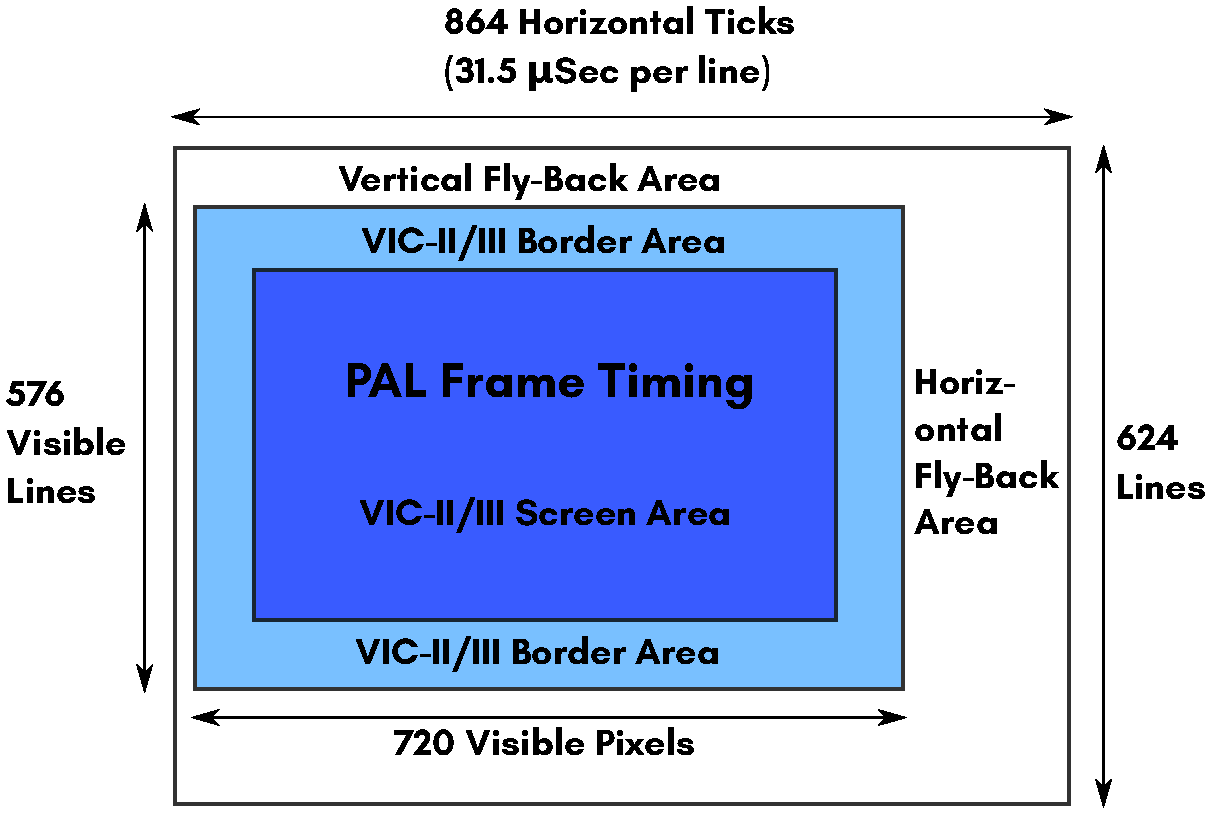
\includegraphics[width=\linewidth]{images/illustrations/VIC-IV-PAL-Frame.pdf}

The NTSC frame is constructed from 526 physical raster lines, consisting of 858 pixel clock ticks. The pixel clock is 27MHz, which is 1/3 the VIC-IV pixel clock.  The visible frame is 720$\times$480 pixels, the entirety of which can be used in VIC-IV mode. In VIC-II and VIC-III modes, the border area reduces the usable size to 640$\times$400 pixels.  In VIC-II mode and VIC-III 200H modes, the display is double scanned, with two 32 micro-second physical rasters corresponding to a single 64 micro-second VIC-II-style raster line.  Thus each frame consists of 263 VIC-II raster lines of 64 micro-seconds each, matching the most common C64 NTSC video timing.

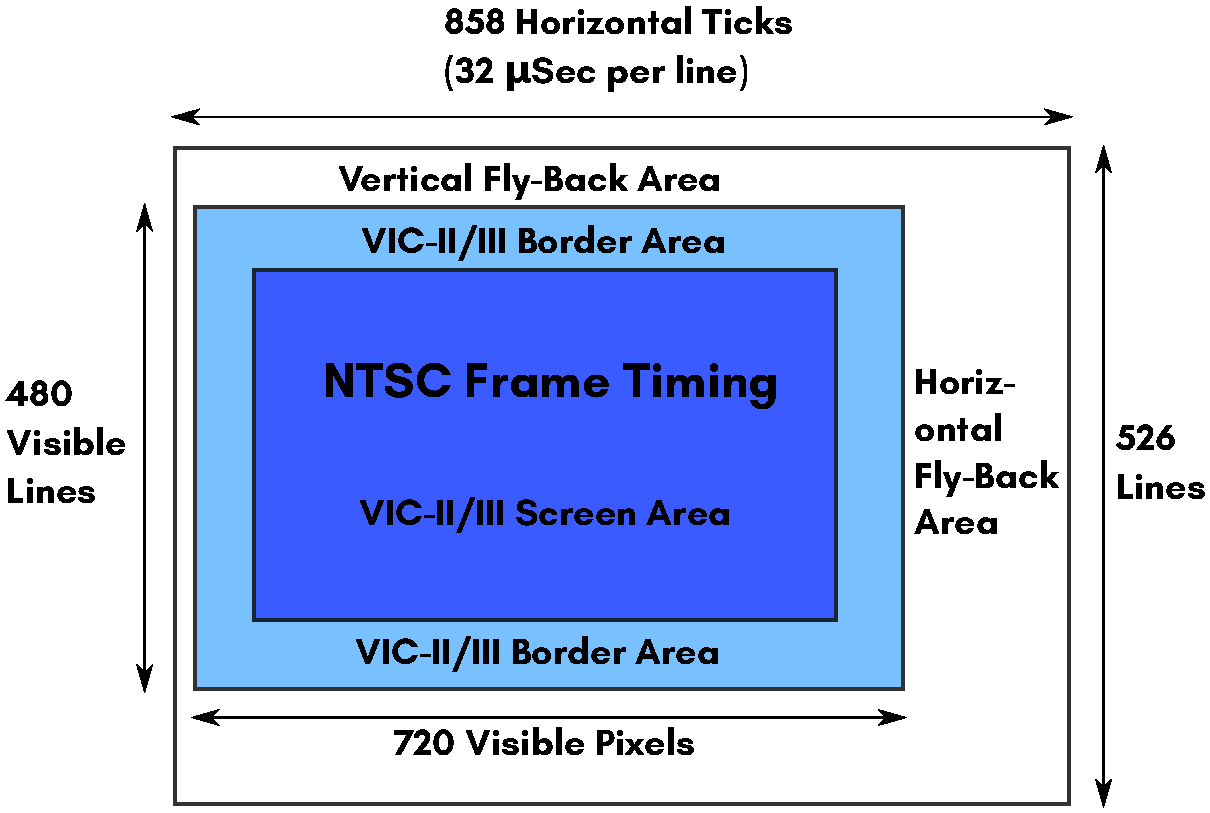
\includegraphics[width=\linewidth]{images/illustrations/VIC-IV-NTSC-Frame.pdf}

As these HDTV video modes are not supported by all VGA monitors, a compatibility mode is included that provides a 640$\times$480 VGA-style mode. However, as the pixel clock of the MEGA65 is fixed at 27MHz, this mode runs at 63Hz.  Nonetheless, this should work on the vast majority of VGA monitors.  There should be no problem with the PAL / NTSC modes when using the digital video output of the MEGA65 with the vast majority of IMDH\texttrademark-enabled monitors and TVs.

To determine whether the MEGA65 is operating in PAL or NTSC, you can enter the freeze menu, which displays the current video mode, or from a program you can check the PALNTSC signal (bit 7 of \$D06F, 53359 decimal). If this bit is set, then the machine is operating in NTSC mode, and clear if operating in PAL mode. This bit can be modified to change between the modes, e.g.:

\begin{tcolorbox}[colback=black,coltext=white]
\verbatimfont{\codefont}
\begin{verbatim}
10 IFPEEK(53272)<32THENPOKE53295,ASC("G"):POKE53295,ASC("S"):REM ENABLE C65+MEGA65 IO
20 NTSC=PEEK(53359)AND128
30 IFNTSCTHENPRINT"MEGA65 IS IN NTSC MODE"
40 IFNTSC=0THENPRINT"MEGA65 IS IN PAL MODE"
50 INPUT"SWITCH MODES (Y/N)? ",A$
60 IFA$="Y"THENPOKE53359,PEEK(53359)+128-NTSC
70 NTSC=PEEK(53359)AND128
80 IFNTSCTHENPRINT"MEGA65 IS NOW IN NTSC MODE"
90 IFNTSC=0THENPRINT"MEGA65 IS NOW IN PAL MODE"
\end{verbatim}
\end{tcolorbox}

\subsubsection{Physical and Logical Rasters}

Physical rasters per frame refers to the number of actual raster lines in the PAL or
NTSC Enhanced Definition TV (EDTV) video modes used by the MEGA65.  Logical Rasters refers to the number of VIC-II-style rasters per frame.
Each logical raster consists of two physical rasters per line, since EDTV modes are double-scan modes compared with the original PAL and NTSC
Standard Definition TV modes used by the C64. The frame parameters of the VIC-IV for PAL and NTSC are as follows:

\setlength{\tabcolsep}{3pt}
\begin{longtable}{|L{2cm}|L{2.5cm}|L{2.5cm}|L{2.5cm}|}
\hline
{\bf{Standard}} & {\bf{Cycles per Raster}} & {\bf{Physical Rasters per Frame}} & {\bf{Logical Rasters per Frame}}  \\
\hline
\endfirsthead
\multicolumn{3}{l@{}}{\ldots continued}\\
\hline
{\bf{Standard}} & {\bf{Cycles per Raster}} & {\bf{Physical Rasters per Frame}} & {\bf{Logical Rasters per Frame}}  \\
\endhead
\multicolumn{3}{l@{}}{continued \ldots}\\
\endfoot
\hline
\endlastfoot
\small PAL & 63 & 312 & 626 \\
\small NTSC & 65 & 263 & 526 \\
\end{longtable}

The result is that the frames on the VIC-IV consist of exactly the same
 number of $\sim$ 1MHz CPU cycles as on the VIC-II exactly.

\subsubsection{Bad Lines}

The VIC-IV does not natively incur any ``bad lines'', because the VIC-IV has its own dedicated memory busses to the main memory
and colour RAM of the MEGA65.  This means that both the processor and VIC-IV can access the memory at the same time, unlike on the
C64 or C65, where they are alternated.

However, to improve compatibility, the VIC-IV signals when a ``bad line'' would have occurred on the VIC-II.  The 45GS02 processor
of the MEGA65 accepts these bad line signals, and pauses the CPU for 40 clock cycles, except if the processor is running
at full speed, in which case they are ignored.  This improves the timing compatibility with the VIC-II considerably.  However,
the timing is not exact, because the current revision of the 45GS02 pauses for exactly 40 cycles, instead of 40 -- 43 cycles,
depending on the instruction being executed at the time. Also, the VIC-IV and 45GS02 do not currently pause for sprite fetches.


The bad line emulation is controlled by bit 0 of \$D710: setting this bit enables bad line emulation, and clearing it prevents
any bad line from stealing time from the processor.


\section{Memory Interface}

The VIC-IV supports up to 64KB of colour RAM and, in principle, 16MB of direct access RAM for video data.  However in typical installations
32KB of colour RAM and 384KB of addressable RAM is present. In MEGA65 systems, the second 128KB of RAM is typically used to hold a C65-compatible ROM, leaving 256KB available, unless software is written to avoid the need to use C65 ROM routines, in which case all 384KB can be used.

The VIC-IV supports all legacy VIC-II and VIC-III methods for accessing this RAM, including the VIC-II's use of 16KB banks, and the VIC-III's Display Address Translator (DAT).  This additional memory can be used for character and bitmap displays, as well as for sprites.  However, the VIC-III bitplane modes remain limited to using only the first 128KB of RAM, as the VIC-IV does not enhance the bitplane mode.

\subsection{Relocating Screen Memory}

To use the additional memory for screen RAM, the screen RAM start address can be adjusted to any location in memory with byte-level granularity by setting the SCRNPTR registers (\$D060 -- \$D063, 53344 -- 53347 decimal).  For example, to set the screen memory to address 12345:

\begin{tcolorbox}[colback=black,coltext=white]
\verbatimfont{\codefont}
\begin{verbatim}
IFPEEK(53272)<32THENPOKE53295,ASC("G"):POKE53295,ASC("S"):REM ENABLE C65+MEGA65 IO
POKE53344+0,69:POKE53344+1,35:POKE53344+2,1
\end{verbatim}
\end{tcolorbox}

\subsection{Relocating Character Generator Data}

The location of the character generator data can also be set with byte-level precision via the CHARPTR registers at \$D068 -- \$D06A (53352 -- 53354 decimal). As usual, the first of these registers holds the lowest-order byte, and the last the highest-order byte. The three bytes allow for placement of character data anywhere in the first 16MB of RAM. For systems with less than 16MB of RAM accessible by the VIC-IV, the upper address bits should be zero.

For example, to indicate that character generator data should be sourced beginning at \$41200 (266752 decimal), the following
could be used.  Note that the AND binary operator only works with arguments between 0 and 65,535. Therefore we first
subtract 4$\times$65,536 = 262,144 from the address (the 4 is determined by calculating INT(266752/65536) ), before we use the AND operator to compute the lower part of the address:

\begin{tcolorbox}[colback=black,coltext=white]
\verbatimfont{\codefont}
\begin{verbatim}
IFPEEK(53272)<32THENPOKE53295,ASC("G"):POKE53295,ASC("S"):REM ENABLE C65+MEGA65 IO
POKE53352,(266752-INT(266752/65536)*65536)AND255
POKE53353,INT((266752-INT(266752/65536)*65536)/256)
POKE53354,INT(266752/65536)
\end{verbatim}
\end{tcolorbox}


\subsection{Relocating Colour / Attribute RAM}

The area of colour RAM being used can be similarly set using the COLPTR registers (\$D064 -- \$D065, 53348 -- 53349 decimal). That is, the value is an offset from the start of the colour / attribute RAM.  This is because, like on the C64, the colour / attribute RAM of the MEGA65 is a separate memory component, with its own dedicated connection to the VIC-IV.  By default, the COLPTRs are set to zero, which replicates the behaviour of the VIC-II/III.  To set the display to use the colour / attribute RAM beginning at offset 4000, one could use something like:

\begin{tcolorbox}[colback=black,coltext=white]
\verbatimfont{\codefont}
\begin{verbatim}
IFPEEK(53272)<32THENPOKE53295,ASC("G"):POKE53295,ASC("S"):REM ENABLE C65+MEGA65 IO
POKE53348,4000 AND 255
POKE53349,INT(4000/256)
\end{verbatim}
\end{tcolorbox}

\subsection{Relocating Sprite Pointers and Images}

The location of the sprite pointers can also be moved, and sprites can be made to have their data anywhere in first 4MB of memory.
This is accomplished by first setting the location of the sprite pointers by setting the SPRPTRADR registers (\$D06C -- \$D06E, 53356 -- 53358 decimal, but note that only the bottom 7 bits of \$D06E are used, as the highest bit is used for the SPRPTR16 signal).  This allows the list of
eight sprite pointers to be moved from the end of screen RAM to an arbitrary location in the first 8MB of RAM.  To allow sprites themselves
to be located anywhere in the first 4MB of RAM, the SPRPTR16 bit in \$D06E must be set. In this mode, two bytes are used to indicate the
location of each sprite, instead of one. That is, the list of sprite pointers will be 16 bytes long, instead of 8 bytes long as on the VIC-II/III.  When SPRPTR16 is enabled, the location of the sprite pointers should always be set explicitly via the SPRPTRADR registers.
For example, to position the sprite pointers at location 800 -- 815, you could use something like the following code. Note that a little gymnastics is required to keep the SPRPTR16 bit unchanged, and also to work around the AND binary operator not working with values greater than 65535:

\begin{tcolorbox}[colback=black,coltext=white]
\verbatimfont{\codefont}
\begin{verbatim}
IFPEEK(53272)<32THENPOKE53295,ASC("G"):POKE53295,ASC("S"):REM ENABLE C65+MEGA65 IO
POKE53356,(800-INT(800/65536)*65536) AND 255
POKE53357,INT(800/256)AND255
POKE53358,(PEEK(53358)AND128)+INT(800/65536)
\end{verbatim}
\end{tcolorbox}

The location of each sprite image remains a multiple of 64 bytes, thus allowing for up to 65,536 unique sprite images
to be used at any point in time, if the system is equipped with sufficient RAM (4MB or more).  In this mode, the VIC-II 16KB banking is ignored, and the location of sprite data is simply 64 $\times$ the pointer value.  For example, to have the data for a sprite at \$C000 (49152 decimal), this would be sprite location 768, because 49152 divided by 64 = 768.  We then need to split 768 into high and low bytes, to set the two pointer bytes: 768 = 256$\times$3, with remainder 0, so this would require the two sprite pointer bytes to be 0 (low byte, which comes first) and 3 (high byte).  Thus if the sprite pointers were located at \$7F8 (2040 decimal), setting the first sprite to sprite image 768 could be done with something like:

\begin{screenoutput}
POKE2040,INT(768/256)
POKE2041,768-256*INT(768/256)
\end{screenoutput}

\section{Hot Registers}

Because of the availability of precise vernier registers to set a wide
range of video parameters directly, \$D011 (53265 decimal), \$D016 (53272 decimal) and other VIC-II and
VIC-III video mode registers are implemented as virtual registers:
by default, writing to any of these results in computed consistent values being
applied to all of the relevant vernier registers.  This means that
writing to any of these virtual registers will reset the video mode.
Thus some care has to be taken when using new VIC-IV features to not
touch any of the ``hot'' VIC-II and VIC-III registers.

The ``hot'' registers to be careful with are:

\$D011, \$D016, \$D018, \$D031 (53265, 53272, 53274 and 53287 decimal) and the VIC-II bank bits of \$DD00 (56576 decimal).

If you write to any of those, various VIC-IV registers will need to be re-written
with the values you wish to maintain.

This ``hot'' register behaviour is intended primarily for legacy software.
It can be disabled by clearing the HOTREG signal (bit 7 of \$D05D, 53341 decimal).

\section{New Modes}

\subsection{Why the new VIC-IV modes are Character and Bitmap modes, not Bitplane modes}

The new VIC-IV video modes are derived from the VIC-II character and bitmap modes, rather than the VIC-III
bitplane modes. This decision was based on several realities of programming a memory-constrained 8-bit home computer:

\begin{enumerate}
\item Bitplanes require that the same amount of memory is given to each area on screen, regardless of whether it
is showing empty space, or complex graphics. There is no way with bitplanes to reuse content from within an image in
another part of the image.  However, most C64 games use highly repetitive displays, with common elements appearing in various
places on the screen, of which Boulder Dash and Super Giana Sisters would be good examples.

\item Bitplanes also make it difficult to update a display, because every pixel is unique, in that there is no way to make a change,
for example to the animation in an onscreen element, and have it take effect in all places at the same time. The diamond
animations in Boulder Dash are a good example of this problem.  The requirement to modify multiple separate bytes in each
bitplane create an increased computational burden, which is why there were calls for the Amiga AAA chip-set to include so-called
``chunky'' modes, rather than just bitplane based modes.  While the Display Address Translator (DAT) and DMAgic of the C65 provide some
relief to this problem, the relief is only partial.

\item Scrolling using the C65 bitplanes requires copying the entire bitplane, as the hardware support for smooth scrolling does not
extend to changing the bitplane source address in a fine manner.  Even using the DMAgic to assist, scrolling a 320$\times$200 256-colour
display requires 128,000 clock cycles in the best case (reading and writing 320$\times$200 = 64000 bytes). At 3.5MHz on the C65 this
would require about 36 milli-seconds, or about 2 complete video frames.  Thus for smooth scrolling of such a display, a double
buffered arrangement would be required, which would consume 128,000 of the 131,072 bytes of memory.

In contrast, the well known character modes of the VIC-II are widely used in games, due to their ability to allow a small amount
of screen memory to select which 8$\times$8 block of pixels to display, allowing very rapid scrolling, reduced memory consumption, and
effective hardware acceleration of animation of common elements.  Thus the focus of improvements in the VIC-IV has been on
character mode.  As bitmap mode on the VIC-II is effectively a special case of character mode, with implied character numbers, it
comes along free for the ride on the VIC-IV, and will only be mentioned in the context of a very few bitmap-mode specific
improvements that were trivial to make, and it thus seemed foolish to not implement, in case they find use.

\end{enumerate}

\subsection{Displaying more than 256 unique characters via
"Super-Extended Attribute Mode"}

The primary innovation is the addition of the Super-Extended Attribute Mode. The VIC-II already uses 12 bits per character: Each 8$\times$8
cell is defined by 12 bits of data: 8 bits of screen RAM data, by
default from \$0400 -- \$07E7 (1024 -- 2023 decimal), indicating which
characters to show, and 4 bits of colour data from the 1K nibble colour
RAM at \$D800 -- \$DBFF (55296 -- 56319 decimal). The VIC-III of the
C65 uses 16 bits, as the colour RAM is now 8 bits, instead of 4, with
the extra 4 bits of colour RAM being used to support attributes (blink,
bold, underline and reverse video).  It is recommended to revise how
this works, before reading the following. A good introduction to the
VIC-II text mode can be found in many places.
% For example, \ref{vicii-cheaper-by-the-dozen}. <- undefined
Super-Extended Attribute mode doubles the number of bits per character used from the VIC-III’s 16, to 32: Two bytes of screen RAM and two bytes of
colour/attribute RAM.

Super-Extended Attribute Mode is enabled by setting bit 0 in \$D054
(53332 decimal). Remember to first enable VIC-IV mode, to make this
register accessible. When this bit is set, two bytes are used for each
of the screen memory and colour RAM for each character shown on the
display. Thus, in contrast to the 12 bits of information that the C64
uses per character, and the 16 bits that the VIC-III uses, the VIC-IV
has 32 bits of information.  How those 32 bits are used varies slightly
among the particular modes.  The default is as follows:

\setlength{\tabcolsep}{3pt}
\begin{longtable}{|L{3cm}|L{8cm}|}
\hline
{\bf{Bit(s)}} & {\bf{Function}}  \\
\hline
\endfirsthead
\multicolumn{2}{l@{}}{\ldots continued}\\
\hline
{\bf{Bit(s)}} & {\bf{Function}}  \\
\endhead
\multicolumn{2}{l@{}}{continued \ldots}\\
\endfoot
\hline
\endlastfoot
\small Screen RAM byte 0 & {\small Lower 8 bits of character number, the same as the VIC-II and VIC-III }\\
\small Screen RAM byte 1, bits 0 - 4 & {\small Upper 5 bits of character number, allowing addressing of 8,192 unique characters }\\
\small Screen RAM byte 1, bits 5 - 7 & {\small Trim pixels from right side of character (bits 0 - 2) }\\
\small Colour RAM byte 0, bit 7 & {\small Vertically flip the character }\\
\small Colour RAM byte 0, bit 6 & {\small Horizontally flip the character }\\
\small Colour RAM byte 0, bit 5 & {\small Alpha blend mode (leave 0, discussed later) }\\
\small Colour RAM byte 0, bit 4 & {\small GOTO X (allows repositioning of characters along a raster via the Raster-Rewrite Buffer, discussed later) }\\
\small Colour RAM byte 0, bits 3 & {\small If set, Full-Colour characters use 4 bits per pixel and are 16 pixels wide (less any right side trim bits), instead of using 8 bits per pixel. When using 8 bits per pixels, the characters are the normal 8 pixels wide  }\\
\small Colour RAM byte 0, bits 2 & {\small Trim pixels from right side of character (bit 3) }\\
\small Colour RAM byte 0, bits 0 - 1 & {\small Number of pixels to trim from top or bottom of character }\\
\small Colour RAM byte 1, bits 0 - 3 & {\small Low 4 bits of colour of character }\\
\small Colour RAM byte 1, bit 4 & {\small Hardware blink of character (if VIC-III extended attributes are enabled) }\\
\small Colour RAM byte 1, bit 5 & {\small Hardware reverse video enable of character (if VIC-III extended attributes are enabled)* }\\
\small Colour RAM byte 1, bit 6 & {\small Hardware bold attribute of character (if VIC-III extended attributes are enabled)* }\\
\small Colour RAM byte 1, bit 7 & {\small Hardware underlining of character (if VIC-III extended attributes are enabled) }\\
\end{longtable}


* Enabling BOLD and REVERSE attributes at the same time on the MEGA65 selects an alternate palette, effectively allowing 512 colours on screen, but each 8$\times$8 character can use colours only from one 256 colour palette.

We can see that we still have the C64 style bottom 8 bits of the character number in the first screen byte. The second byte of screen memory gets five extra bits for that, allowing 2$^{13}$ = 8,192 different characters to be used on a single screen. That's more than enough for unique characters covering an 80$\times$50 screen (which is possible to create with the VIC-IV).  The remaining bits allow for trimming of the character.  This allows for variable width characters, which can be used to do things that would not normally be possible, such as using text mode for free horizontal placement of characters (or parts thereof). This was originally added to provide hardware support for proportional width fonts.

For the colour RAM, the second byte (byte 1) is the same as the C65, i.e., the lower half providing four bits of foreground colour, as on the C64, plus the optional VIC-III extended attributes. The C65 specifications document describes the behaviour when more than one of these are used together, most of which are logical, but there are a few combinations that behave differently than one might expect. For example, combining bold with blink causes the character to toggle between bold and normal mode. Bold mode itself is implemented by effectively acting as bit 4 of the foreground colour value, causing the colour to be drawn from different palette entries than usual.

The C65 / VIC-III attributes and the use of 256 colour 8-bit values for various VIC-II colour registers is enabled by setting bit 5 of \$D031 (53297 decimal).  Therefore this is highly recommended when using the VIC-IV mode, as otherwise certain functions will not behave as expected. Note that BOLD+REVERSE together has the meaning of selecting an alternate palette on the MEGA65, which differs from the C65.

Many effects are possible due to Super-Extended Attribute Mode.  A few possibilities are explained in the following sub-sections.

\subsection{Using Super-Extended Attribute Mode}

Super-Extended Attribute Mode requires double the screen RAM and colour RAM as the VIC-II/III text modes. This is because two bytes of each are
required to define each character, instead of one.  The screen RAM can be located anywhere in the 384KiB of main memory using registers \$D060 -- \$D062 (53344 -- 53346 decimal).  The colour RAM can be located anywhere in the 32KiB colour RAM.  Only the first 1 or 2 KiB of the colour RAM is visible at \$D800 -- \$DBFF or \$D800 -- \$DFFF (if the {\em CRAM2K} signal is set in bit 0 of \$D030, 53296 decimal). Thus if using a screen larger than 40$\times$25 characters use of the DMA controller or some other means may be required to access the full amount of colour RAM.  Thus we will initially discuss using Super-Extender Attribute Mode with a 40x25 character display.

The easiest way to use Super-Extended Attribute Mode is from C65 mode, with the screen set to 80 columns, as the C65 ROM sets up 2KiB for both the screen RAM and colour RAM.  The user need only to treat each character pair as a single Super-Extended Attribute character.

The first step is to enable the Super-Extended Attribute Mode by asserting the {\em FCLRHI} and {\em CHR16} signals, by setting bits 2 and 0 of \$D054 (53332 decimal).  As this is a VIC-IV register, we must first enable the VIC-IV IO mode.  The VIC-IV must also be configured to 40 column mode, by clearing the {\em H640} signal by clearing bit 7 of \$D031 (53297 decimal).  This is because each pair of characters will be used to form a single character on screen, thus 80 bytes are required to display 40 characters.

Because pairs of colour RAM and screen RAM bytes are used to define each character, care must be taken to initialise and manipulate the screen.
A good approach is to set the text colour to black, because this is colour code 0, and then to fill the screen with @ characters, because that is
character code 0.  You can then have several ways to manipulate the screen.  You can use the normal PRINT command and carefully construct
strings that will put the correct values into each screen and colour byte pair. Another approach is to use the BANK and POKE commands to directly set the contents of the screen and colour RAM.


XXX Finish above description

XXX Example program

The following descriptions assume that you have implemented one of the methods described above to set the screen and colour RAM.

\subsection{Full-Colour (256 colours per character) Text Mode}

In normal VIC-II/III text mode, one byte is used for each row of pixels in a character.  As a reminder for how those modes work, in
hi-res mode, each pixel is either the background or foreground colour, based on the state of one bit in the byte.  Multi-colour mode
uses two bits to select between four possible colours, but as there are still only 8 bits to describe each row of 8 pixels, each pair
of pixels has the same colour.

The VIC-IV's full-colour text mode removes these limitations, and allows each pixel of a character to be chosen from the 256 colour of
either the primary or alternate palette bank.  To do this, each character now requires 64 bytes of data.  Also,
XXX

\subsection{Many-colour (16 colours per character) Text Mode}

XXX

\subsection{Alpha-Blending / Anti-Aliasing}

XXX

\subsection{Flipping Characters}

XXX

\subsection{Variable Width Fonts}

There are 4 bits that allow trimming pixels from the right edge of characters when they are displayed. This has the effect of making
characters narrower. This can be useful for making more attractive text displays, where narrow characters, such as ``i'' take less space than wider characters, such as ``m'', without having to use a bitmap display. This feature can be used to make it very efficient to display
such variable-width text displays -- both in terms of memory usage and processing time.

This feature can be combined with full-colour text mode, alpha blending mode and 4-bits per pixel mode to allow characters that consist of
15 levels of intensity between the background and foreground colour, and that are up to 16 pixels wide.  Further, the GOTO bit can be used to implement negative kerning, so that character pairs like A and T do not have excessive white space between them when printed adjacently. The prudent use of these features can result in highly impressive text display, similar to that on modern systems, but that are still efficient enough to be implemented on a relatively constrained system such as the MEGA65. The ``MegaWAT!?'' presentation software for the MEGA65 uses several of these features to produce its attractive anti-aliased proportional text display on slides.

XXX Example program

\subsection{Raster-Rewrite Buffer}

If the GOTO bit is set for a character in Super-Extended Attribute Mode, instead of painting a character, the position on the raster is back-tracked (or advanced forward to) the
pixel position specified in the low 10 bits of the screen memory bytes.  If the vertical flip bit is set, then this has the alternate
meaning of preventing the background colour from being painted.  This combination can be used to print text material over the top of
other text material, providing a crude supplement to the 8 hardware sprites.  The amount of material is limited only by the raster
time of the VIC-IV. Some experimentation will be required to determine how much can be achieved in PAL and NTSC modes.

This ability to draw multiple layers of text and graphics is highly powerful. For example, it can be used to provide multiple overlapping
layers of separately scrollable graphics.  This gives many of the advantages of bitplane-based play-fields on other computers, such as the
Amiga, but without the disadvantages of bitplanes.

XXX Example program

\section{Sprites}

\subsection{VIC-II/III Sprite Control}

The control of sprites for C64 / VIC-II/III compatibility is unchanged from the C64.  The only practical differences are very minor.
In particular the VIC-IV uses ring-buffer for each sprites data when rendering a raster. This means that a sprite can be displayed multiple times per raster line, thus potentially allowing for horizontal multiplexing.

\subsection{Extended Sprite Image Sets}

On the VIC-II and VIC-III, all sprites must draw their image data from a single 16KB region of memory at any point in time.
This limits the number of different sprite images to 256, because each sprite image occupies 64 bytes.  In practice, the same
16KB region must also contain either bitmap, text or bitplane data, considerably reducing the number of sprite images that
can be used at the same time.

The VIC-IV removes this limitation, by allowing sprite data to be placed anywhere in memory, although still on 64-byte
boundaries. This is done by setting the SPRPTR16 signal (bit 7, \$D06E, decimal 53358), which tells the VIC-IV to expect
two bytes per sprite pointer instead of one.  These addresses are then absolute addresses, and ignore the 16KB VIC-II
bank selection logic.  Thus 16 bytes are required instead of 8 bytes.  The list of pointers can also be placed anywhere
in memory by setting the SPRPTRADR (\$D06C -- \$D06D, 53356 -- 53357 decimal) and SPRPTRBNK signals (bits 0 -- 6, \$D06E, 53358 decimal).
This allows for sprite data to be located anywhere in the first 4MB of RAM, and the sprite pointer list to be located anywhere
in the first 8MB of RAM.  Note that typical installations of the VIC-IV have only 384KB of connected RAM, so these limitations are
of no practical effect. However, the upper bits of the SPRPTRBNK signal should be set to zero to avoid forward-compatibility
problems.

One reason for supporting more sprite images is that sprites on the VIC-IV can require more than one 64 byte image slot.
For example, enabling Extra-Wide Sprite Mode means that a sprite will require 8$\times$21 = 168 bytes, and will thus occupy
four VIC-II style 64 byte sprite image slots.  If variable height sprites are used, this can grow to as much as  8$\times$255 = 2,040 bytes per sprite.

\subsection{Variable Sprite Size}

Sprites can be one of three widths with the VIC-IV:

\begin{enumerate}
\item Normal VIC-II width (24 pixels wide).
\item Extra Wide, where 64 bits (8 bytes) of data are used per raster line, instead of the VIC-II's 24.
  This results in sprites that are 64 pixels wide, unless Full-Colour Sprite Mode is selected for a sprite,
  in which case the sprite will be 64 / 8 = 8 pixels wide.
\item Tiled mode, where the sprite is drawn repeatedly until the end of the raster line.
\end{enumerate}

To enable a sprite to be 64 pixels (or 16 pixels if in Full-Colour Sprite Mode), set the corresponding bit for the sprite in the SPRX64EN register at (\$D057, 53335 decimal).

Similarly, sprites can be various heights:  Sprites will be either the 21 pixels high of the VIC-II, or if the corresponding bit for the sprite is enabled in the SPRHGTEN signal (\$D055, 53333 decimal), then that sprite will be the number of pixels tall that is set in the SPRHGT
register (\$D056, 53334 decimal).

\subsection{Variable Sprite Resolution}

By default, sprites are the same resolution as on the VIC-II, i.e., each sprite pixel is two physical pixels wide and high.
However, sprites can be made to use the native resolution, where sprite pixels are one physical pixel wide and/or high.
This is achieved by setting the relevant bit for the sprite in the SPRENV400 (\$D076, 53366 decimal) registers to increase the
vertical resolution on a sprite-by-sprite basis.  The horizontal resolution for all sprites is either the normal VIC-II resolution, or if the SPR640 signal
is set (bit 4 of \$D054, 53332 decimal), then sprites will have the same horizontal resolution as the physical pixels of the display.

\subsection{Sprite Palette Bank}

The VIC-IV has four palette banks, compared with the single palette bank of the VIC-III.
The VIC-IV allows the selection of separate palette banks for bitmap/text graphics and for sprites.  This makes it easy to have
very colourful displays, where the sprites have different colours to the rest of the display, or to use palette animation to achieve
interesting visual effects in sprites, without disturbing the palette used by other elements of the display.

The sprite palette bank is selected by setting the SPRPALSEL signal in bits 2 and 3 of the register \$D070 (53360 decimal).
It is possible to set this to the same bank as the bitmap/text display, or to select a different palette bank.
Palette bank selection takes effect immediately.  Don't forget that to be able to modify a palette, you have to also bank it
to be the palette accessible via the palette bank registers at \$D100 -- \$D3FF by setting the MAPEDPAL signal in bits 6 and 7 of
\$D070.

\subsection{Full-Colour Sprite Mode}

In addition to monochrome and multi-colour modes, the VIC-IV supports a new full-colour sprite mode.  In this mode, four bits are used to
encode each sprite pixel.  However, unlike multi-colour mode where pairs of bits encode pairs of pixels, in full-colour mode the pixels
remain at their normal horizontal resolution.  The colour zero is considered transparent. If you wish to use black in a full-colour sprite, you must configure the palette bank that is selected for sprites so that one of the 15 colours for the specific sprite encodes black.

Full-colour sprite mode is selectable for each sprite by setting the appropriate bit in the SPR16EN register (\$D06B, 53355 decimal).

To enable the eight sprites to have 15 unique colours each, the sprite colour is drawn using the palette entry corresponding to:
$sprite number \times 16 + nibble value$, where $sprite number$ is the number of the sprite (from 0 to 7), and $nibble value$ is the value
of the half-byte that contains the sprite data for the pixel.  In addition, if bitplane mode is enabled for this sprite, then 128 is
added to the colour value, which makes it easy to switch between two colour schemes for a given sprite by changing only one bit in the
SPRBPMEN register.

Because Full-Colour Sprite Mode requires four bits per pixel, sprites will be only six pixels wide, unless Extra Wide Sprite Mode is enabled
for a sprite, in which case the sprite will be 16 pixels wide.  Tiled Mode also works with Full-Colour Sprite Mode, and will result in the
16 full-colour pixels of the sprite being repeated until the end of the raster line.

The following BASIC program draws a Full-Colour Sprite in either C64 or C65 mode:

\begin{screenoutput}
0 AD=56*64:IF PEEK(53272) AND 32 THEN GOTO 30: REM C65/C64 MODE DETECT
10 POKE 53295,ASC("G"):POKE 53295,ASC("S"): REM ENABLE MEGA65 VIC-IV FEATURES
20 AD=768+64: REM $0340 HEX FOR SPRITE
30 FOR I=AD TO AD+168:POKEI,0:NEXT I
40 POKE 2040,AD/64: REM SET SPRITE NUMBER
50 POKE 53269,1: REM ENABLE SPRITE 0
60 POKE 53248,100:POKE 53249,100: REM PUT SPRITE ON SCREEN
70 POKE 53355,1: REM MAKE SPRITE 0 16-COLOUR
80 POKE 53335,1: REM MAKE SPRITE 0 USE 64 BITS OF DATA = 16 X 4-BIT PIXELS
90 POKE 53287,10: REM MAKE PINK THE TRANSPARENT COLOUR
100 GOSUB 900: REM READ MULTI-COLOUR SPRITE

899 END

900 REM LOAD SPRITE
910 READN$:IFN$="END"THEN RETURN
920 GOSUB 1000
930 GOTO 910

1000 REM DECODE STRING OF NIBBLES IN N$ AT ADDRESS AD
1010 L=LEN(N$)
1020 FOR I=1 TO (L/2+1):POKE AD+I,0
1030 FOR I= 1 TO L:N=ASC(MID$(N$,I,1))-ASC("@")
1040 A=AD+INT((I-1)/2):IF (I AND 1)=1 THEN N=N*16
1050 V=PEEK(A):POKE A,V OR N:NEXTI
1060 AD=AD+INT(I/2)
1070 IF (L AND 1) THEN AD=AD+1
1080 RETURN

1998 REM SPRITE DATA FOLLOWS
1999 REM @ = TRANSPARENT, A-O = COLOURS 1 TO 15
2000 DATA "@ABCDEFGHIJKLMNO"
2010 DATA "AA@@@@@@@@@@@@@@"
2020 DATA "A@A@@@@@@@@@@@@@"
2030 DATA "A@@A@@@@@@@@@@@@"
2040 DATA "A@@@A@@@@@@@@@@@"
2050 DATA "A@@@@A@@@@@@@@@@"
2060 DATA "A@@@@@A@@@@@@@@@"
2070 DATA "A@@@@@@A@@@@@@@@"
2080 DATA "A@@@@@@@A@@@@@@@"
2090 DATA "A@@@@@@@@A@@@@@@"
2100 DATA "A@@@@@@@@@A@@@@@"
2110 DATA "A@@@@@@@@@@A@@@@"
2120 DATA "A@@@@@@@@@@@A@@@"
2130 DATA "A@@@@@@@@@@@@A@@"
2140 DATA "A@@@@@@@@@@@@@A@"
2150 DATA "A@@@@@@@@@@@@@@A"
2160 DATA "A@@@@@@@@@@@@@@@"
2170 DATA "A@@@@@@@@@@@@@@@"
2180 DATA "A@@@@@@@@@@@@@@@"
2190 DATA "A@@@@@@@@@@@@@@@"
2200 DATA "A@@@@@@@@@@@@@@@"
2210 DATA "END"
\end{screenoutput}

\section{VIC-II / C64 Registers}

\input{regtable_VIC-II.C64}

\section{VIC-III / C65 Registers}

\input{regtable_VIC-III.C65}

\section{VIC-IV / MEGA65 Specific Registers}

\input{regtable_VIC-IV.MEGA65}

  \chapter{6526 Complex Interface Adaptor (CIA) Registers}

\section{CIA 6526 Registers}

\subsection*{CIA1 Registers}
\input{regtable_CIA1.C64}

\subsection*{CIA2 Registers}
\input{regtable_CIA2.C64}

\section{CIA 6526 Hypervisor Registers}

In addition to the standard CIA registers available on the C64 and C65, the MEGA65
provides an additional set of registers that are visible only when the system is in
Hypervisor Mode. These additional registers allow the internal state of the CIA to
be more fully extracted when freezing, thus allowing more programs to function
correctly after being frozen.  They are not visible when using the MEGA65 normally,
and can be safely ignored by programmers who are not programming the MEGA65 in
Hypervisor Mode.

\subsection*{CIA1 Hypervisor Registers}
\input{regtable_CIA1.MEGA65}

\subsection*{CIA2 Hypervisor Registers}
\input{regtable_CIA2.MEGA65}

  \chapter{4551 UART, GPIO and Utility Controller}

\section{C65 6551 UART Registers}

\input{regtable_UART.C65}

\section{4551 General Purpose I/O \& Miscellaneous Interface Registers}
\label{sec:uartmisc}

\input{regtable_UARTMISC.MEGA65}

  \chapter{45E100 Fast Ethernet Controller}

\section{Overview}

The 45E100 is a new and simple Fast Ethernet controller that has been
designed specially for the MEGA65 and for 8-bit computers generally.
In addition to supporting 100Mbit Fast Ethernet, it is radically
different from other Ethernet controllers, such as the RR-NET.

The 45E100 includes dual receive buffers, allowing one frame to be
processed while another is receiving.  It includes automatic CRC32
checking on reception, and automatic CRC32 generation for transmit, considerably
reducing the burden on the processor and allowing for very simple programs.  It also supports true
full-duplex operation at 100Mbit per second, allowing for total bi-directional
throughput exceeding 100Mbit per second.  The MAC address is software
configurable, and promiscuous mode is supported, as are individual control
of the reception of broadcast and multi-cast Ethernet frames.  The 45E100 also
supports both transmit and receive interrupts, allowing greatly improved
real-world performance. When especially low latency is required, it is also possible
to immediately abort the transmission of the current Ethernet frame, so that a
higher-priority frame can be immediately sent.
These features combine to enable sub-millisecond round trip latencies,
which can be of particular value for interactive applications, such as multi-player network
games.

\subsection{Differences to the RR-NET and similar solutions}

The RR-NET and other Ethernet controllers for the Commodore\texttrademark \ line
of 8-bit home computers generally use an Ethernet controller that was
designed for 16-bit PCs, but that also supports a so-called ``8-bit mode,''
which suffers from a number of disadvantages. The primary disadvantages
are the lack of working interrupts, and processor intensive access to
the Ethernet frame buffers.  The lack of interrupts forces programs to
use polling to check for the arrival of new Ethernet frames.  This,
together with the complexities of accessing the buffers results in an
Ethernet interface that is very slow, and whose real-world throughput
is considerably less than its theoretical 10Mbits per second.  Even
a Commodore 64 with REU cannot achieve speeds above several tens of
kilobytes per second.

In contrast, the 45E100 supports both RX (Ethernet frame received) interrupts and TX
(ready to transmit) interrupts, freeing the processor from having to poll
the device. Because the 45E100 supports RX interrupts, there is no need for large
numbers of receive buffers, which is why the 45E100 requires only two RX buffers
to achieve very high levels of performance.

Further, the 45E100 supports direct memory mapping of the
Ethernet frame buffers, allowing for much more efficient access, including
by DMA.  Using the MEGA65's integrated DMA controller it is quite possible
to achieve transfer rates of several mega-bytes per second -- some 100x
faster than the RR-NET.

\subsection{Theory of Operation: Receiving Frames}

The 45E100 is simple to operate: To begin receiving Ethernet frames, the programmer
needs only to clear the RST bit (bit 0 of register \$D6E0) to release the
Ethernet controller from reset.  It will then auto-negotiate connection at
the highest available speed, typically 100Mbit, full-duplex.  The RXBLKD bit (bit 6 of \$D6E0)
should then be checked, and if set, the RXBM (bit 2 of register \$D6E1) bit should be toggled to switch
the active and mapped receive buffers, so that the 45E100 knows that the
program no longer needs the contents of the previously mapped buffer, and can
safely begin receiving an Ethernet frame into that buffer.

When the 45E100 receives an ethernet frame, it will assert RXBLKD to indicate that the receive
buffer has been filled with an ethernet frame.  No further ethernet frames will be received until
RXBLKD is cleared again, as described above. This is because the 45E100 has only two receive buffers
for ethernet frames: one of which is mapped visible to the processor, and the other which is visible
to the 45E100's ethernet engine at any point in time.  Toggling RXBM allows toggling between which
of the two buffers is mapped and which is ready to receive an ethernet frame.  The buffers are 2KiB
bytes each.  The first two bytes are used to indicate the length of the received frame, and four
are consumed by the ethernet CRC32 code, yielding an effective Maximum Transport Unit (MTU) length
of 2,042 bytes.  The ethernet frame data begins at byte offset 2 in the receive buffer, with the
frame length written LSB-first in the first two bytes.  The layout of the receive buffers is thus as follows:

\begin{longtable}{|L{1.0cm}|L{1.1cm}|C{1.3cm}|L{6.9cm}|}
\hline
{\bf{HEX}} & {\bf{DEC}} & {\bf{Length}} & {\bf{Description}} \\
\hline
\endfirsthead
\multicolumn{3}{l@{}}{\ldots continued}\\
\hline
{\bf{HEX}} & {\bf{DEC}} & {\bf{Length}} & {\bf{Description}} \\
\hline
\endhead
\multicolumn{3}{l@{}}{continued \ldots}\\
\endfoot
\hline
\endlastfoot
\small  0000 & \small 0 & 1 & The low byte of the length of the received ethernet frame. \\
\hline
\small  0001 & \small 1 & 1 & The lower four bits contain the upper bits of the length of the received ethernet frame.  Bit 4 is set if the received ethernet frame is a multi-cast frame. Bit 5 if it is a broadcast frame. Bit 6 is set if the frame's destination address matches the 45E100's programmed MAC address. Bit 7 is set if the CRC32 check for the received frame failed, i.e., that the frame is either truncated or was corrupted in transit. \\
\hline
\small  0002 -- 07FB & \small 2 -- 2,043 & 2,042 & The received frame. Frames shorter than 2,042 bytes will begin at offset 2. \\
\hline
\small  07FC -- 07FF & \small 2,044 -- 2,047 & 4 & Reserved space for holding the CRC32 code during reception.  The CRC32 code is, however, always located directly after the received frame, and thus will only occupy this space if the received frame is more than 2,038 bytes long. '' \\
\hline
\end{longtable}

Because of the very rapid rate at which Fast Ethernet frames can be received, a programmer should use the
receive interrupt feature, enabled by setting RXQEN (bit 7 of \$D6E1).  Polling is possible as an alternative, but
is not recommended with the 45E100, because at the 100Mbit Fast Ethernet speed, packets can arrive
as often as every 10 microseconds.  Fortunately, at the MEGA65's 40MHz full speed mode, and using
the 20MiB per second DMA copy functionality, it is possible to keep up with such high data rates.

\subsection{Accessing the Ethernet Frame Buffers}

Unlike on the RR-NET, the 45E100's ethernet frame buffers are able to be memory mapped, allowing rapid access via DMA
or through assembly language programs.  It is also possible to access the buffers from BASIC with some care.

The frame buffers can either be accessed from their natural location in the MEGA65's extended address space at address
\$FFDE800 -- \$FFDEFFF, or they can be mapped into the normal C64/C65 \$D000 IO address space.  Care must be
taken as mapping the ethernet frame buffers into the \$D000 IO address space causes all other IO devices to unavailable
during this time.  Therefore interrupts MUST be disabled before doing so, whether using BASIC or machine code.  Therefore
when programming in assembly language or machine code, it is recommended to use the natural location, and to access this
memory area using one of the three mechanisms for accessing extended address space, which are described in Appendix
\ref{sec:extended-memory}.

The method of
disabling interrupts differs depending on the context in which a program is being written. For programs being written using C64 mode's BASIC 2, the following will work:

\begin{screenoutput}
  POKE56333,127: REM DISABLE CIA TIMER IRQS
\end{screenoutput}

While for C65's BASIC 10, the following must instead be used, because a VIC-III raster interrupt is used instead of a CIA-based timer interrupt:

\begin{screenoutput}
POKE53274,0: REM DISABLE VIC-II/III/IV RASTER IRQS
\end{screenoutput}

Once this has been done, the IO context for the ethernet controller can be activated by writing \$45 (69 in decimal, equal to the character 'E' in PETSCII)) and \$54 (84 in decimal, equal to the character 'T' in PETSCII) into the VIC-IV's KEY register (\$D02F, 53295 in decimal), for example:

\begin{screenoutput}
POKE53295,ASC("E"):POKE53295,ASC("T")
\end{screenoutput}

At this point, the ethernet RX buffer can be read beginning at location \$D000 (53248 in decimal), and the TX buffer can be written to at the same address.  Refer to `Theory of Operation: Receiving Frames' above for further explanation on this.

Once you have finished accessing the ethernet frame buffer, you can restore the normal C64, C65 or MEGA65 IO context by writing to the VIC-III/IV's KEY register.  In most cases, it will make the most sense to revert to the MEGA65's IO context by writing \$47 (71 decimal) in and \$53 (83 in decimal) to the KEY register, for example:

\begin{screenoutput}
POKE53295,ASC("G"):POKE53295,ASC("S")
\end{screenoutput}

Finally, you should then re-enable interrupts, which will again depend on whether you are programming from C64 or C65 mode.  For C64 mode:

\begin{screenoutput}
POKE56333,129
\end{screenoutput}

For C65 mode it would be:

\begin{screenoutput}
POKE53274,129
\end{screenoutput}



\subsection{Theory of Operation: Sending Frames}

Sending frames is similarly simple: The program must simply load the frame to be transmitted into
the transmit buffer, write its length into TXSZLSB and TXSZMSB registers, and then write \$01 into
the COMMAND register.  The frame will then begin to transmit, as soon as the transmitter is idle.
There is no need to calculate and attach an ethernet CRC32 field, as the 45E100 does this automatically.

Unlike for the receiver, there is only one frame buffer for the transmitter (this may be changed in
a future revision). This means that you cannot prepare the next frame until the previous frame has
already been sent.  This slightly reduces the maximum data throughput, in return for a very simple
architecture.

Also, note that the transmit buffer is write-only from the processor bus interface. This means that
you cannot directly read the contents of the transmit buffer, but must load values ``blind''.  Finally,
the 45E100 allows you to send ethernet.

\subsection{Advanced Features}

In addition to operating as a simple and efficient ethernet frame transceiver, the 45E100
includes a number of advanced features, described here.

\subsubsection{Broadcast and Multicast Traffic and Promiscuous Mode}

The 45E100 supports filtering based on the destination Ethernet address, i.e., MAC address.
By default, only frames where the destination Ethernet address matches the ethernet address
programmed into the MACADDR1 -- MACADDR6 registers will be received. However, if the MCST bit
is set, then multicast ethernet frames will also be received. Similarly, setting the BCST bit
will allow all broadcast frames, i.e., with MAC address ff:ff:ff:ff:ff:ff, to be received.
Finally, if the NOPROM bit is cleared, the 45E100 disables the filter entirely, and will
receive all valid ethernet frames.

\subsubsection{Debugging and Diagnosis Features}

The 45E100 also supports several features to assist in the diagnosis of ethernet problems.
First, if the NOCRC bit is set, then even ethernet frames that have invalid CRC32 values
will be received. This can help debug faulty ethernet devices on a network.

If the STRM bit is set, the ethernet transmitter transmits a continuous stream of debugging frames
supplied via a special high-bandwidth logging interface. By default, the 45E100 emits a
stream of approximately 2,200 byte ethernet frames that contain compressed video provided
by a VIC-IV or compatible video controller that supports the MEGA65 video-over-ethernet
interface.  By writing a custom decoder for this stream of ethernet frames, it is possible
to create a remote display of the MEGA65 via ethernet. Such a remote display can be used,
for example, to facilitate digital capture of the display of a MEGA65.

The size and content of the debugging frames can be controlled by writing special values to the
COMMAND register.  Writing \$F1 allows the selection of frames that are ~1,200 bytes long.
While this reduces the performance of the debugging and streaming features, it allows the reception
of these frames on systems whose ethernet controllers cannot be configured to receive frames
of ~2,200 bytes.

If the STRM bit is set and bit 2 of \$D6E1 is also set, a compressed log of instructions executed by
the 45gs02 CPU will instead be streamed, if a compatible processor is connected to this interface.
This mechanism includes back-pressure, and will cause the 45gs02 processor to slowdown,
so that the instruction data can be emitted.  This typically limits the speed of the connected
45gs02 processor to around 5MHz, depending on the particular instruction mix.

Note also that
the status of bit 2 of \$D6E1 cannot currently be read directly. This may be corrected in a future
revision.

Finally, if the video streaming functionality is enabled, this also enables reception of synthetic
keyboard events via ethernet.  These are delivered to the MEGA65's Keyboard Complex Interface Adapter
(KCIA), allowing full remote interaction with a MEGA65 via its ethernet interface.  This feature is
primarily intended for development.

\section{Memory Mapped Registers}

The 45E100 Fast Ethernet controller is a MEGA65-specific feature.
It is therefore only available in the MEGA65 IO context.
This is enabled by writing \$53 and then \$47 to VIC-IV register \$D02F.
If programming in BASIC, this can be done with:

\begin{screenoutput}
POKE53295,ASC("G"):POKE53295,ASC("S")
\end{screenoutput}

The 45E100 Fast Ethernet controller has the following registers

\setlength{\tabcolsep}{3pt}
\begin{longtable}{|L{1.2cm}|L{1.1cm}|c|c|c|c|c|c|c|c|}
\hline
{\bf{HEX}} & {\bf{DEC}} & {\bf{DB7}} & {\bf{DB6}} & {\bf{DB5}} & {\bf{DB4}} & {\bf{DB3}} & {\bf{DB2}} & {\bf{DB1}} & {\bf{DB0}} \\
\hline
\endfirsthead
\multicolumn{3}{l@{}}{\ldots continued}\\
\hline
{\bf{HEX}} & {\bf{DEC}} & {\bf{DB7}} & {\bf{DB6}} & {\bf{DB5}} & {\bf{DB4}} & {\bf{DB3}} & {\bf{DB2}} & {\bf{DB1}} & {\bf{DB0}} \\
\endhead
\multicolumn{3}{l@{}}{continued \ldots}\\
\endfoot
\hline
\endlastfoot
\small  D6E0 & \small 55008 & \small -- & \small RXBLKD & \small -- & \small KEYEN & \small DRXDV & \multicolumn{2}{c|}{\small DRXD}& \small RST \\
\hline
\small  D6E1 & \small 55009 & \small RXQEN & \small TXQEN & \small RXQ & \small TXQ & \small STRM & \small RXBU & \small RXBM & \small -- \\
\hline
\small  D6E2 & \small 55010 & \multicolumn{8}{c|}{\small TXSZLSB}\\
\hline
\small  D6E3 & \small 55011 & \multicolumn{8}{c|}{\small TXSZMSB}\\
\hline
\small  D6E4 & \small 55012 & \multicolumn{8}{c|}{\small COMMAND}\\
\hline
\small  D6E5 & \small 55013 & \multicolumn{2}{c|}{\small --}& \small MCST & \small BCST & \multicolumn{2}{c|}{\small TXPH}& \small NOCRC & \small NOPROM \\
\hline
\small  D6E6 & \small 55014 & \multicolumn{3}{c|}{\small MIIMPHY}& \multicolumn{5}{c|}{\small MIIMREG}\\
\hline
\small  D6E7 & \small 55015 & \multicolumn{8}{c|}{\small MIIMVLSB}\\
\hline
\small  D6E8 & \small 55016 & \multicolumn{8}{c|}{\small MIIMVMSB}\\
\hline
\small  D6E9 & \small 55017 & \multicolumn{8}{c|}{\small MACADDR1}\\
\hline
\small  D6EA & \small 55018 & \multicolumn{8}{c|}{\small MACADDR2}\\
\hline
\small  D6EB & \small 55019 & \multicolumn{8}{c|}{\small MACADDR3}\\
\hline
\small  D6EC & \small 55020 & \multicolumn{8}{c|}{\small MACADDR4}\\
\hline
\small  D6ED & \small 55021 & \multicolumn{8}{c|}{\small MACADDR5}\\
\hline
\small  D6EE & \small 55022 & \multicolumn{8}{c|}{\small MACADDR6}\\
\hline
\end{longtable}
\begin{itemize}
\item{\bf{BCST}} Accept broadcast frames
\item{\bf{COMMAND}} Ethernet command register (write only)
\item{\bf{DRXD}} Read ethernet RX bits currently on the wire
\item{\bf{DRXDV}} Read ethernet RX data valid (debug)
\item{\bf{KEYEN}} Allow remote keyboard input via magic ethernet frames
\item{\bf{MACADDR1}} Ethernet MAC address
\item{\bf{MACADDR2}} Ethernet MAC address
\item{\bf{MACADDR3}} Ethernet MAC address
\item{\bf{MACADDR4}} Ethernet MAC address
\item{\bf{MACADDR5}} Ethernet MAC address
\item{\bf{MACADDR6}} Ethernet MAC address
\item{\bf{MCST}} Accept multicast frames
\item{\bf{MIIMPHY}} Ethernet MIIM PHY number (use 0 for Nexys4, 1 for MEGA65 r1 PCBs)
\item{\bf{MIIMREG}} Ethernet MIIM register number
\item{\bf{MIIMVLSB}} Ethernet MIIM register value (LSB)
\item{\bf{MIIMVMSB}} Ethernet MIIM register value (MSB)
\item{\bf{NOCRC}} Disable CRC check for received packets
\item{\bf{NOPROM}} Ethernet disable promiscuous mode
\item{\bf{RST}} Write 0 to hold ethernet controller under reset
\item{\bf{RXBLKD}} Indicate if ethernet RX is blocked until RX buffers rotated
\item{\bf{RXBM}} Set which RX buffer is memory mapped
\item{\bf{RXBU}} Indicate which RX buffer was most recently used
\item{\bf{RXQ}} Ethernet RX IRQ status
\item{\bf{RXQEN}} Enable ethernet RX IRQ
\item{\bf{STRM}} Enable streaming of CPU instruction stream or VIC-IV display on ethernet
\item{\bf{TXPH}} Ethernet TX clock phase adjust
\item{\bf{TXQ}} Ethernet TX IRQ status
\item{\bf{TXQEN}} Enable ethernet TX IRQ
\item{\bf{TXSZLSB}} TX Packet size (low byte)
\item{\bf{TXSZMSB}} TX Packet size (high byte)
\end{itemize}


\subsection{COMMAND register values}

The following values can be written to the COMMAND register to perform the described functions.
In normal operation only the STARTTX command is required, for example, by performing the following POKE:

\begin{screenoutput}
POKE55012,1
\end{screenoutput}

\begin{longtable}{|L{1.2cm}|L{1.1cm}|C{2cm}|L{6cm}|}
\hline
{\bf{HEX}} & {\bf{DEC}} & {\bf{Signal}} & {\bf{Description}} \\
\hline
\endfirsthead
\multicolumn{3}{l@{}}{\ldots continued}\\
\hline
{\bf{HEX}} & {\bf{DEC}} & {\bf{Signal}} & {\bf{Description}} \\
\hline
\endhead
\multicolumn{3}{l@{}}{continued \ldots}\\
\endfoot
\hline
\endlastfoot
\small  0000 & \small 0 & STOPTX & Immediately stop transmitting the current ethernet frame.  Will cause a partially sent frame to be received, most likely resulting in the loss of that frame.   \\
\hline
\small  0001 & \small 1 & STARTTX & Transmit packet \\
\hline
\small  00D0 & \small 208 & RXNORMAL & Disable the effects of RXONLYONE \\
\hline
\small  00D4 & \small 212 & DEBUGVIC & Select VIC-IV debug stream via ethernet when \$D6E1.3 is set \\
\hline
\small  00DC & \small 220 & DEBUGCPU & Select CPU debug stream via ethernet when \$D6E1.3 is set \\
\hline
\small  00DE & \small 222 & RXONLYONE & Receive exactly one ethernet frame only, and keep all signals states (for debugging ethernet sub-system) \\
\hline
\small  00F1 & \small 241 & FRAME1K & Select ~1KiB frames for video/cpu debug stream frames (for receivers that do not support MTUs of greater than 2KiB) \\
\hline
\small  00F2 & \small 242 & FRAME2K & Select ~2KiB frames for video/cpu debug stream frames, for optimal performance. \\
\hline
\end{longtable}


\section{Example Programs}

Example programs for the ethernet controller exist in imperfect for in the MEGA65 Core repository on github in the src/tests and src/examples directories.

  \chapter{45IO27 Multi-Function IO Controller}

\section{Overview}

The 45IO27 is a multi-purpose IO controller that incorporates the functions of the
C65's F011 floppy controller, together with the MEGA65's SD card controller interface,
and a number of other miscellation IO functions.

Each of these major functions is covered in a separate section of this chapter

\section{F011-compatible Floppy Controller}

The MEGA65 computer is one of very few modern computers that still
includes first-class support for magnetic floppy drives.  It includes
a floppy controller that is backwards compatible with the C65's F011D
floppy drive controller.

However, unlike the F011D, the MEGA65's
floppy disk controller supports HD and ED media, and similar to the
1541 floppy drive, it also supports variable data rates, so that a
determined user could develop disk formats that store more data,
includ robust copy protection schemes, or both.

GCR encoding is not currently supported, but may be supported by a
future revision of the controller.  It may also be possible with some
creativity and effort to use the debug register interface to read
double-density GCR formatted media.  This is because there are debug
registers that can be queried to indicate the gap between each
successive magnetic domain -- which is sufficient to decode any disk
format. 

\subsection{Multiple Drive Support}

Like the C65's F011 floppy drive controller, the 45IO27 supports up to 8 drives.
The first two of those drives, drive 0 and drive 1, are assumed to be connected to a
standard 34-pin floppy cable, the same as used in standard PCs, i.e.,
with a twist in the cable to allow the use of two unjumpered drives.

As is described in later sections, it is possible to switch drive 0
and drive 1's position, without having to change cabling. Similarly,
either or both of the first two drives may reference a real floppy
drive, a D81 disk image stored on an attached SD card, or redirected
to the floppy drive virtualisation service, so that the sector
accesses can be handled by a connected computer, e.g., as part of a
comfortable and efficient cross-development environment.

The remaining six drives are supported only in conjunction with a
future C1565-compatible external drive port.

\subsection{Buffered Sector Operations}
\label{subsec:reading-from-disks-and-buffer-management}

The 45IO27 support two main modes of reading sectors from a
disk: byte-by-byte, and via a memory-mapped sector buffer.

The byte-by-byte mechanism consists of having a loop wait for the DRQ
signal to be asserted, and then reading the byte of data from the DATA
register (\$D087).

The memory-mapped sector buffer method consists of waiting for the
BUSY flag to clear, indicating that the entire sector has been read,
and then directly accessing the sector buffer located at \$FFD6C00 --
\$FFD6DFF. Care should be taken to ensure that the BUFSEL signal (bit 7 of \$D689) is
cleared, so that the floppy sector buffer is visible, rather than the
SD card sector buffer for programmes other than the Hypervisor. This
is because only the Hypervisor has access to the full 4KiB SD
controller buffer space: Normal programmes see either the floppy
sector buffer or the SD card sector buffer repeated 8 times between
\$FFD6000 and \$FFD6FFF.

Alternatively, the sector buffer can be mapped at \$DE00 -- \$DFFF,
i.e., in the 4KB IO area, by writing the \$81 to the SD command
register at \$D680.  This will hide any IO peripherals that are
otherwise using this area, e.g., from cartridges, or REU emulation.
This function can be disabled again by writing \$82 to the SD command
register. As with the normal sector buffer memory mapping at
\$FFD6xxx, the BUFSEL signal (bit 7 of \$D689) affects whether the FDC
or the SD card sector buffer is visible, for software not running in
Hypervisor mode.  Note that if you use the matrix mode / serial monitor
interface to inspect the contents of the sector buffer, that this occurs
in the Hypervisor context, and so the BUFSEL signal will be ignored,
and the full 4KiB buffer will be visible.

The memory-mapped sector buffer has the advantage that it can be
accessed via DMA, allowing for very efficient copies.  Also, it allows
for loading a sector to occur in the background, while your program
gets on with more interesting things in the meantime.

\subsection{Reading Sectors from a Disk}

There are several steps that you must follow in order to successfully read
a sector from a disk. If you follow these instructions, your code will work
with both physical disks, as well as D81 disk images that exist on the SD
card:

\begin{itemize}
\item First, enable the motor and select the appropriate drive. The F011
  supports upto 8 physical drives, although it is rare for more than two
  to be physically connected.  To enable the motor, write \$60 to \$D080.
  You should then write a SPINUP command (\$20) to \$D081, and wait for
  the BUSY flag (bit 7 of \$D082) to clear.  The drive is now spinning
  at speed, and ready to service requests.
\item Next, select the correct side of the disk by either setting or clearing
  the SIDE1 flag (bit 3 of \$D080).  This takes effect immediately.
\item Third, use the step-in and step-out commands (writing \$10 and \$18 to
  \$D081) as required to move the head to the correct track. Again, after each
  command, you should wait for the BUSY flag (bit 7 of \$D082) to clear, before
  issuing the next command.

  Note that you can check if the head is at track 0
  by checking the TRACK0 flag, but there is no fool-proof way to know if you
  are on any other specific track.  You can use the registers at \$D6A3 --
  \$D6A5 to see the track, sector and side value from the last sector header
  which passed under the head to make an informed guess as to which track
  is currently selected. Note that this only works for real disks, as disk
  images do not spin under the read head. Also note that it is possible for
  tracks to contain sectors which purposely or accidently have incorrect
  track numbers in the sector headers.
  
  \item Fourth, you need to load the desired track, sector and
side number into the TRACK, SECTOR and SIDE registers (\$D084, \$D085
and \$D086, respectively). The FDC is now primed ready to read a sector.

\item Fifth, you should write an appropriate read command
value into \$D081.  This will normally be \$40 (64).  You then wait
for the RDREQ signal (\$D083, bit 7) to go high, to indicate that the
sector has been found. You then either wait for each occassion when
DRQ goes high, and read byte-by-byte in such a loop, or wait for the
BUSY flag to clear and the DRQ and EQ flags to go high, which indicates
that the complete sector has been read into the buffer.

\end{itemize}

\subsection{Track Auto-Tune Function Deprecated}

The 45IO27 also includes a track ``auto-tune'' function, which is enabled
by clearing bit 7 of \$D696.  That function reads the sector headers to
determine which track the head is currently over, and steps the head in or
out to try to get to the correct track. Auto-tune is enabled by default.

\subsection{Sector Skew and Target Any Mode}

It is also worth noting that the TARGANY signal can be asserted to
tell the floppy controller to simply read the next sector that passes
under the head.  This applies only when using real floppy disks, where
it offers the considerable advantage of letting you read the sectors
in the order in which they exist on the disk. This allows you to read
a track at once, without having to wait for the index hole to pass by,
or having to know which sector will next pass under the head.

For example,
the C65 DOS formats disks using a skew factor of 7, while PCs may use
a different skew-factor. If you don't know the skew factor of the disk,
you may schedule the reading of the sectors on the track in a sub-optimal
order. This can result in transfer rates as low as 5 sectors per second,
compared with the optimal case of 50 sectors per second.
Thus with either correct sector order, or using the target any mode,
it is possible to read approximately two full tracks per second,
i.e., two sides $\times$ two tracks, or approximately 20KiB/second on
DD disks, or double that on HD disks, at around 40KiB/second.  This
compares very favourably with the C65 DOS loading speed, which is
typically nearer 1KiB/sec in C64 mode.

\subsection{Disk Layout and 1581 Logical Sectors}

The 1581 disk format is unusual in that the physical sectors on the
disk are a different size of the size of the data blocks that it
presents to the user.  Specifically, the disks use 512 byte sectors,
while the 1581 (and C65) DOS present 256 byte data blocks.
Two blocks are stored in each physical sector.  Also, the physical
track numbers are from 0 to 79, while the logical track numbers of the
DOS are 1 to 80.  Physical sectors are also numbered from 1 to 10,
while logical block numbers begin are 0 to 39.

This means that if you want to find a 1581 logical sector, you need to
know which physical sector it will be found in.  To determine the
physical sector that contains a block, you first subtract one from the
track number, and then divide the sector number by two.  Logical
sectors 0 to 19 of each track are located in physical sectors 1 to 10
on the first side of the disk.  Logical sectors 20 to 39 are 
located in physical sectors 1 to 10 on the reverse side of the disk.  

Thus we can map a some logical track and sector $t$,$s$ to the
physical track, side and sector as follows:

$track = t - 1$

$sector = (s/2)+1, IFF s < 20, ELSE = ((s-20)/2) + 1$

$side = 0 IFF sector < 20$

It is also worth noting that the 45IO27 is capable of reading from
tracks beyond track 80, provided that the disk drive is capable of
this.  Almost all 3.5 inch floppy drives are capable of reading at
least one extra track, as historically manufacturers of floppy disks
stored information about the disk on the 81st track.  In our
experience almost all drives will also be able to access an 82nd
track.

\subsection{FD2000 Disks}

The CMD(tm) FD2000(tm) high-density 3.5'' disk drives for Commodore(tm) computers
use an unusual disk layout that is quite different from PCs: They use 10 sectors,
the same as on 720KB double-density (DD) disks, but double the {\em sector size}
from 512 bytes to 1,024 bytes.  The 45IO27 does not currently support these
larger sectors. At least read-only support is planned to be added via a core update
in the future.

However, the 45IO27 {\em does} already support high-density disks and drives, with much
higher capacities than the FD2000 was able to support.

\subsection{High-Density and Variable-Density Disks}

The 45IO27 supports variable data rates, allowing the use of HD drives and media,
with a flexible approach to disk formats to support user experimentation, and the
easy manipulation of high-capacity software distribution formats.

You are really only limited by your imagination, available time, and
the limited number of people who are still interested in inserting a
floppy disk into their computer!

The standard high-density (HD) disk format is ``1.44MB'', using 18 sectors per track over 80 tracks.
This results in 80 tracks $\times$ 18 sectors $\times$ 2 sides = 2,880 sectors. As each sector
is 512 bytes, this corresponds to 1,440 KiB.  This leads us into the interesting wonderland of
``floppy disk marketing megabytes,'' a phenomena which long predates SD card and hard drive
manufacturers using 1,000,000 byte megabytes.

Curiously for floppy disks, the 1,024,000 byte ``mega byte'' was used, i.e., ``1MB'' = 1 KiB $\times$ 1 KB,
that is a strange hybrid of binary and decimal conventions.  Perhaps it was because the previous standard
was 720KB, and they thought people would thing it odd if double 720KB was 1.41MiB, and complain about the
missing kilo-bytes.  We will continue to use the 1,024KB = 1,000KiB floppy disk marketing mega-byte for
consistency with this historical inconsistency.

However, HD floppy disks are fundamentally capable of holding much more than 1.44MB. For example, the FD2000
stored 1.6MB by using double-sized sectors to squeeze the equivalent of 20 sectors per track, and the Amiga
went further by using track-at-once writing to fit 22 sectors per track. Both these formats used a constant
data rate over all tracks, and thus a constant number of sectors per track.

However, the circumference of the tracks on a 3.5'' floppy disk vary quite a lot: The inner track has a diameter
of around 2.5cm, while the outside track is 1.6$\times$ longer. 
The 1.44MB disk format is designed so that
the data is reliably stored on those shorter inner tracks.
This means that we should be able to fit 160\%
more data on the outer-most track compared with the inner-most track, subject to a number of terms and conditions
imposed by The Laws of Physics, the design of floppy drive electronics, the quality of media being used and
various other annoying things.
Because of this variability and uncertainty, the MEGA65's floppy controller supports fully variable data rate
on a track-by-track basis.

\subsection{Track Information Blocks}

To support variable data rates, the 45GS27 supports the use of
{\em Track Information Blocks}\index{Track Information Block} (TIBs)\index{TIB} that contain information on the
data rate and encoding used on the track. This allows users to experiment with various densities on various tracks,
and yet have the disks function automatically for buffered sector operations.

The Track Information Block is automatically created when using the automatic track format function, but must be
manually created if using unbuffered formatting. The TIB itself consists of the following data:

\begin{enumerate}
\item 3$\times$ \$A1 Sync bytes (written with clock byte \$FB)
\item \$65 MEGA65 Track Information Block marker (written with clock byte \$FF, as are all following bytes in the block)
\item The track number
\item The data rate divisor, in the same format as \$D6A2, i.e., data rate = 40.5MHz / value.
\item Track encoding information: Bit 7 = Track-at-once flag, 1 = no inter-sector gaps (Amiga style), 0 = with inter-sector gaps (normal), Bit 6 = data encoding, 0 = MFM, 1=RLL2,7. Other bits are reserved, and should be 0 when written.
\item Sector count, i.e., number of sectors on the track.
\item CRC byte 1, using the normal floppy disk CRC algorithm.
\item CRC byte 2, using the normal floppy disk CRC algorithm.
\end{itemize}

The Track Information Block is always written a the data rate for a 720KB Double-Density disk,
so that they can be present on any disk.  Writing the Track Information Block and start-of-track
gaps at the DD data rate also ensures that at very high data rates, the head still has sufficient
time to switch to write mode, thus avoiding one of the many problems that arise when writing data
at very high data rates.

If formatting disks unbuffered, it is the programmer's responsibility to switch the data rate after
having written the Track Information Block, and several more bytes to allow the floppy encoding
pipeline to flush out the last byte of the Track Information Block.
This is all automatically managed if using the automatic track formatting function.

The inclusion of the TIB allows users to play and explore the possibilities of different data rates
on different drives and media, while still being automatically readable in all MEGA65s, because the
TIB allows the controller to switch to the correct data rate and encoding.  It is likely that over
time somewhat standardised formats will develop, quite likely in the range of 2MB to 3.5MB -- thus
approaching the capacity of ED media in ED drives, without the need for those drives or media.

\subsection{Formatting Disks}

Formatting disks is now possible with the 45IO27, either unbuffered or fully-automatic.
To format a track issue one of the following commands to \$D081:

\begin{itemize}
\item \$A0 -- Automatic format, with inter-sector gaps, and write pre-compensation disabled.
\item \$A1 -- Manual format, write-precompensation disabled.
\item \$A4 -- Automatic format, with inter-sector gaps, and write pre-compensation enable.
\item \$A5 -- Manual format, write-precompensation enabled.
\item \$A8 -- Automatic format, Amiga-style track-at-once, and write pre-compensation disabled.
\item \$AC -- Automatic format, Amiga-style track-at-once, and write pre-compensation enable.
\end{itemize}  
  
Manual formatting is not recommended, unless mastering track-at-once formatted disks for software
distribution, because of the relative complexity of doing so. Also, at the higher data rates,
bytes have to be delivered to the floppy controller as often as every 20 cycles, which requires
considerable care when writing the format routine.
For more information on manual formatting tracks, refer to the C64 Specifications Manual or the
C65 ROM DOS source code, for examples of manual formatting.

The automatic modes, in contrast, format a track with a single command, and are thus much easier to use,
and are recommended for general use.  Write pre-compensation should normally be enabled, as it is
required at higher data rates, and does not cause problems at lower data rates.

\subsection{Write Pre-Compensation}

Write pre-compensation is a family of algorithms used when writing high data-rate signals to floppy disks.
It is used to anticipate and cancel out the predictable component of timing variation of magnetic recording.
There are a variety of sources of this timing variation, which have been the subject of PhD theses, and a
lot of proprietary research by hard drive manufacturers.  What is important for us to understand is that adjacent
pulses (really magnetic inversions) get pushed together, if they are surrounded by longer pulses, or tend to
spread apart if surrounded by shorter pulses.

There are also other fascinatingly complex and difficult to predict factors, that cause things such as the ``negative
shift of mid-length pulses'', ``inverse F-distribution of pulse arrival times'' and goodness knows what else.  But
we shall leave those to the hard drive manufacturers.  We limit ourselves to the data pattern induced effect described
in the previous paragraph.

The 45GS27 supports two tunable coefficients for small and large corrections to this,
which are used with an internal look-up table.  However, this is all automatically handled if you enable write pre-compensation.
This allows data rates that much more closely approach the expected limit of HD media, although due to the other horrors of
magnetic media recording alluded to above, the actual limit is not reached.

\subsection{Buffered Sector Writing}

The 45IO27 can write to disk images that are located on the SD card,
or when using virtualised disk access.

To write a sector, you follow a similar process to reading, except
that you write \$84 to the command byte instead of \$40.  The \$80
indicates a write, and the \$04 activates write-precompensation.  This
is important when writing to real floppy disks, especially HD and ED
disks.  Write-precompensation causes bits to be written slightly early
or slightly late, using an algorithm that models how the magnetic
domains on a disk tend to move after being written.

If you do not wish
to use the sector buffer, but instead provide each byte one at a time
during the write operation, you must add \$01 to the command code.
However, this is not recommended on the MEGA65, because when writing
to the SD card or using virtualised disk images the entire sector
operation can happen instantaneously from the perspective of your
program.  This means that it is not possible to supply data reliably
when in this mode.  Thus apart from being less convenient, it is also
less reliable. 

Once a write operation has been triggered, the DRQ signal indicates
when you should provide the next byte if performing a byte-by-byte
write. Otherwise, it is assumed that you will have pre-filled the
sector buffer with the complete 512 bytes of data required.

To write to disks that contain Track Information Blocks\index{Track Information Block}\index{TIB},
you should first wait for the TIB to be read when changing tracks. This is done by waiting
for \$D6A9 (sectors per track from the TIB) to contain a non-zero value.

\subsection{F011 Floppy Controller Registers}

The following are the set of F011 compatibility registers of the 45IO47.
Note that registers related to the use of SD card based storage are found in the corresponding section below.

\input{regtable_FDC.C65}

The following registers apply to the 45IO27 only, i.e., are MEGA65 specific:

\input{regtable_FDC.MEGA65}

\section{SD Card Controller and F011 Virtualisation Functions}

For those situations where you do not wish to use real floppy disks,
the 45IO27 supports two complementary alternative modes:

\begin{itemize}
\item SD card Based Disk Image Access.
\item Virtualised Disk Image Access.
\end{itemize}

This is in addition to providing direct access to a dual-bus SD card
interface.

\subsection{SD card Based Disk Image Access}

The 45IO27 is both a floppy drive and SD card controller.
This enables it to transparently allow access to D81 disk images
stored on the SD card.  Further, because the controller is combined,
it is possible to still have the floppy drive step and spin as though
it were being used, providing considerable atmosphere and sense of
realism, even when using disk images.

The 45IO27 supports both 800KB standard D81 disk images, as well as
64MiB ``MEGA Images''.  While an operating system may impose
restrictions based on the name of a file, the 45IO27 is blind to these
requirements. Instead, it requires only that a {\tt contiguous} 800KiB
or 64MiB of the SD card is used to contain a disk image.

When a disk image is enabled, the corresponding set of sectors on the
SD card are effectively placed under user control, and the operating
system is no longer able to prevent the reading or writing of any of
those sectors.  Thus you should never enable access to an image that
is shorter than the required size, as it will otherwise allow the user
to unwittingly or maliciously access and/or modify data that is not
part of the image file.

For the same reason, only the hypervisor can change the sector number
where a disk image starts (the D?STARTSEC? signals), or allow the use
of disk images instead of the real floppy drive (USEREAL0 and USEREAL1
signals).  Once the Hypervisor has set the start sector of a disk
image, and cleared the USEREAL0 or USEREAL1 signal, the user can still
controll whether an access will go to the real floppy drive or to the
disk image by respectively clearing or setting the appropriate
signal.  For drive 0, this is D0IMG, and for drive 1, it is D1IMG.

There are also signals to control whether a disk image is an 800KiB
D81 image or a 64MiB MEGA Disk image, and whether a disk image is
present, and whether it is write protected. These are all located in
the \$D68B register. Because of the ability of manipulation of these
registers to corrupt or improperly access data, these signals are all
read-only, except from within the hypervisor.

The following table lists the registers that are used to control
access to disk images resident on the SD card:

\input{regtable_SDFDC.MEGA65}

\subsection{F011 Virtualisation}

In addition to allowing automatic read and write access to SD card
based D81 images, it is possible to connect a program to the serial
monitor interface that provides and accepts data as though it were the
floppy disk.

This is commonly used in a cross-development
environment, where you wish to frequently modify a disk image that is
used by a program you are developing -- without the need to
continually push new versions of the disk image on the MEGA65's
SD card first. It also has the added benefit that it allows you to
easily visualise which sectors are being read from and written to,
which can help speed up development and debugging of your program.

This function operates together with the MEGA65's Hypervisor by
triggering hyperrupts (that is, interrupts that activate the
Hypervisor).  There is then special code in the Hypervisor that
communicates with the {\tt m65} program via the serial monitor
interface.

If that all sounds rather complex, all you need to know is that to use
this function, you run the {\tt m65} utility with arguments like
{\tt -d image.d81}.  This should automatically establish the link with
the MEGA65.  If the BASIC interprettor stops responding, press the
reset button (not the power switch) on the left side of your MEGA65,
and it should return to the BASIC's {\tt READY.} prompt -- and if your
supplied disk image has a C65 auto-boot function, then it should
automatically start booting.

This function works very well if the host computer runs Linux, and
will allow loading at a speed of around 60KiB per second.  However, it
may be much slower on Windows or Apple OSX-based systems.

Of course to use this, you will also need an interface module and/or
cable to connect your cross-development system to the MEGA65's serial
monitor interface. This is most easily done using a Trenz TE0790-03
JTAG adapter and mini-USB cable.

More information on using this interface and the {\tt m65} tool can be
found in \bookvref{cha:transfer-and-debug-tools}.

\subsection{Dual-Bus SD Card Controller}

The 45IO27 contains a high-speed dual-bus SD card controller.  This
controller operates in SPI x1 mode at a clock speed of 20MHz,
providing a maximum throughput of approximately 2MiB/sec.  The quality
of the SD card makes a signficant difference to performance, with some
cards routinely delivering 1.7MiB/sec, while others 1MiB/sec or
less. Generally speaking, newer cards marketted as being suitable for
video recording perform better.  The controller supports SDHC cards,
and has experimental support for SDXC cards.  Legacy SD cards with a
capacity of 2GiB or less are not supported, as these use a different
addressing mode.

The SD controller itself is very simple to drive: Supply the sector
number in \$D861-\$D684, and then issue a read or write command to the
command register (\$D680).  The SD controller supports only
sector-based buffered operations, using the sector buffer. In
hypervisor mode, the sector buffer is located at \$FFD6E00 --
\$FFD6FFF, while when the computer is in normal operating mode, the SD
card and the floppy controller share a single address for both the
floppy drive and SD card sector buffers. Which buffer is visible at
that address is dictated by the BUFSEL signal. If it is 1, then the SD
card buffer is visible, while if it is 0, then the floppy drive sector
buffer is visible.  See also Sub-section
\vref{subsec:reading-from-disks-and-buffer-management} for further
discussion on the precise behaviour of this buffer with regard to
normal mode versus Hypervisor mode, and how it can also be mapped at
\$DE00. 

\subsubsection{Write Gate}

When writing a sector, you must, however, first open the ``write
gate''. This is a mechanism to prevent accidental corruption of data
on the SD card, as it requires two different values to be written to
the command register (\$D680) in quick succession: You have
approximately 1 milli second after opening the write gate to command
the write, before the write gate effectively closes again,
write-protecting the SD card until the write gate is opened again.
There are two different write gates: One for the master boot record
(sector 0), and the other for all other sectors, both of which are
listed in the command table below. This is designed to provide
additional protection to the very important master boot record sector
against programmes accidentally calculating sector 0 as the target for
an ordinary write.

\subsubsection{Fill Mode}

Where you wish to fill sectors with a constant value, the 45IO27
supports a mode for this, so that you do not need to overwrite the
contents of the sector buffer. This is activated by placing the
desired fill value into the FILLVAL register (\$D686), and then
issuing the enable fill mode command (\$83), performing the sector
write operations, and then issuing the disable fill mode command
(\$84). 

\subsubsection{Selecting Among Multiple SD Cards}

The controller supports two SD Card interfaces, and it is possible to
have a card in both at the same time.  However, each card needs to be
reset and commanded separately.  Only one card can be commanded at a
time.  That said, it is possible to reset each card once, and then
switch between the cards to perform individual operations.

To select the first SD Card slot, write \$C0 to the SD Controller
Command Register (\$D680).  To select the second SD Card slot, write
\$C1 instead.

\subsubsection{SD Controller Command Table}

The SD controller supports the following commands that can be written
to the command register at \$D680:

\setlength{\tabcolsep}{3pt}
\begin{longtable}{|L{2.4cm}|L{8cm}|}
\hline
{\bf{Command}} & {\bf{Function}} \\
\hline
\endfirsthead
\multicolumn{2}{l@{}}{\ldots continued}\\
\hline
{\bf{Command}} & {\bf{Function}} \\
\endhead
\multicolumn{2}{l@{}}{continued \ldots}\\
 \endfoot
 \hline
\endlastfoot
\small \$00 (0) & Place SD card under reset (deprecated. Use command
\$10 instead) \\
 \hline
\small \$01 (1) & Release SD card from reset \\
 \hline
\small \$02 (2) & Read a sector from the SD card \\
 \hline
\small \$03 (3) & Write a single sector to the SD card \\
 \hline
\small \$04 (4) & Write the first sector of a multi-sector write to the SD card \\
 \hline
\small \$05 (5) & Write a subsequent sector of a multi-sector write to the SD card \\
 \hline
\small \$06 (6) & Write the final sector of a multi-sector write to the SD card \\
 \hline
\small \$0C (12) & Request flush of SD card write buffers (experimental) \\
 \hline
\small \$0E (14) & Pull SD handshake line low (debug only) \\
 \hline
\small \$0F (15) & Pull SD handshake line high (debug only) \\
 \hline
\small \$10 (16) & Place SD card under reset with flags set (preferred
method) \\
 \hline
\small \$11 (17) & Release SD card from reset (alternate method) \\
 \hline
\small \$40 (64) & Clear the SDHC/SDXC flag, selecting legacy SD card mode (deprecated)  \\
 \hline
\small \$41 (65) & Set the SDHC/SDXC mode flag   \\
 \hline
\small \$44 (68) & End force clearing of SD card state machine error
flag \\
\small \$45 (69) & Begin force clearing of SD card state machine error
flag \\
\small \$4D (77) & Open write-gate to sector 0 (master boot record)
for approximately 1 milli-second \\
 \hline
\small \$57 (87) & Open write-gate for all sectors > 0 for approximately 1 milli-second \\
 \hline
\small \$81 (129) & Enable mapping of the SD/FDC sector buffer at
\$DE00 -- \$DFFF \\
 \hline
\small \$82 (130) & Disable mapping of the SD/FDC sector buffer at
\$DE00 -- \$DFFF \\
 \hline
\small \$83 (131) & Enable SD Card Fill Mode \\
 \hline
\small \$84 (132) & Disable SD Card Fill Mode \\
 \hline
\small \$C0 (192) & Select SD Card Slot 0 \\
 \hline
\small \$C1 (193) & Select SD Card Slot 1 \\
 \hline
   \end{longtable}


Note that the hypervisor can enable or disable direct access to the SD
controller. The hypervisor operating system may provide a mechanism
for requesting permission to access the SD card controller, e.g., for
disk management utilities.

The SD card controller registers are as follows:

\input{regtable_SD.MEGA65}

\section{Touch Panel Interface}

Some MEGA65 variants include an LCD touch panel, primarily the
MEGAphone hand-held version of the MEGA65.  The touch interface
supports the detection of two simultaneous touch events.  Some
variants may also support gesture detection, however, this is still
very experimental.

The touch detection interface that is contained in the 45IO27 is
complemented by the on-screen-keyboard interface of the 4551 UART and
GPIO controller.  Refer to \bookref{sec:uartmisc} for further
information.  Of particular relevance are bit 7 of the registers \$D615 --
\$D617 which allow activating the on-screen keyboard interface,
selecting whether the on-screen keyboard is placed in the upper or
lower portion of the screen, and whether the primary or secondary
on-screen keyboard is displayed.

Direct connections between the 4551 and the 45IO27 combine information
about any currently displayed on-screen keyboard and the touch
interface controller, allowing synthetic keyboard events to be
automatically triggered when the on-screen keyboard portion of the
touch interface is pressed.  This allows the touch interface to be
used to drive the on-screen keyboard without requiring any support
from user programmes. This works even when the on-screen keyboard is
moving during activation or transitioning between the top and bottom
of the screen.

As touch interfaces can require calibration, the 45IO27 allows for a
linear transformation of both the X and Y coordinates of a touch
event.  Specifically, there are scale (TCHXSCALE and TCHYSCALE) and
offset registers (TCHXDELTA and TCHYDELTA) that provide for this
transformation. It is also possible to flip the touch screen
coordinates in either or both the X and Y axes.  These calibration
registers also affect the operation of the on-screen keyboard.

It should also be noted that some touch interfaces do not have
constant horizontal or vertical resolution. For example, some panels
have a low horizontal resolution region in the middle of the panel,
which can require some care to accommodate.

To detect the primary touch event, the TOUCH1XLSB, TOUCH1XMSB, TOUCH1YLSB,
TOUCH1YMSB registers can be read.  Similar registers exist for the 2nd
touch event: TOUCH2XLSB, TOUCH2XMSB, TOUCH2YLSB, TOUCH2YMSB. Each
touch event has a signle bit flag that indicates whether the touch
event is currently valid: the EV1 and EV2 bits of the register
\$D6B0.  There are also corresponding bit-fields that indicate whether a
given touch event has been made or released, allowing the detection of
when a finger both makes and breaks contact with the screen.  The
UPDN1 and UPDN2 signals provide this information.  Binary values of 01 and
10, respectively indicate if the finger has been removed or pressed
against the touch panel.  Values of 00 and 11 mean that a finger is
either being held or not being held against the touch panel.

The
primary touch event is also fed into the lightpen\index{light pen} input of the VIC-IV,
and can be detected using the normal light pen registers of the VIC-IV.

The registers for the touch panel interface are as follows:

\input{regtable_TOUCH.MEGA65}

\section{Audio Support Functions}
\index{cross-bar switch, audio}
\index{mixer, audio}
\index{audio mixer}
\index{audio cross-bar switch}
The 45IO27 provides the primary interface into the MEGA65's full
cross-bar audio mixer. This includes the interface for reading or
modifying the mixer co-efficients, as well as accessing the mixer
feedback registers, and setting the 16-bit digital sample values that
are two of the input channels into the audio mixer.

The audio mixer consists of 128 coefficients, each of which is 16
bits.  Each audio output channel, e.g., left speaker, right speaker,
left headphone, right headphone, cellular modem 1 (MEGAphone models
only) and so on, are generated by taking each of the audio input
channels, multiplying them by the appropriate coefficient, and adding
it to the total output of the audio output channel.

Because each
audio output channel has its own set of coefficients that are applied
to all of the audio input channels, this means that it is possible to
produce totally different audio out each audio channel: For example,
it is possible to play your favourite quadrophonic SID music out of
the headphones while rick-rolling passers by with Amiga-style MOD
audio.  This is why the audio mixer is refered to as a {\tt full
  cross-bar} mixer, because there are no restrictions on how you mix
each audio output channel.  In this regard, it is very similar to a
full-function audio desk, allowing different mixing levels for
different speakers.

Because the audio coefficients are 16 bits each, each one is formed
using two successive bytes of the audio co-efficient space.  Changes
to the audio coefficients take effect immediately, so care should be
taken when changing coefficients to avoid audible clicks and pops.
Also, you must allow 32 cycles to elapse before changing the selected
audio coefficient, as otherwise the change may be discarded if the
audio mixer accumulator has not had time to re-visit that coefficient.

The audio sources on the MEGA65 and MEGAphone devices are as follows:

\setlength{\tabcolsep}{3pt}
\begin{longtable}{|L{2.4cm}|L{8cm}|}
\hline
{\bf{Input Channel ID}} & {\bf{Connection}} \\
\hline
\endfirsthead
\multicolumn{2}{l@{}}{\ldots continued}\\
\hline
{\bf{Input Channel ID}} & {\bf{Connection}} \\
\endhead
\multicolumn{2}{l@{}}{continued \ldots}\\
 \endfoot
 \hline
\endlastfoot
\small \$0 (0) & Left SIDs \\
 \hline
\small \$1 (1) & Right SIDs \\
 \hline
\small \$2 (2) & Modem Bay 1 (MEGAphone only) \\
 \hline
\small \$3 (3) & Modem Bay 2 (MEGAphone only) \\
 \hline
\small \$4 (4) & Bluetooth(tm) Left \\
 \hline
\small \$5 (5) & Bluetooth(tm) Right \\
 \hline
\small \$6 (6) & Headphone Interface 1 \\
 \hline
\small \$7 (7) & Headphone Interface 2 \\
 \hline
\small \$8 (8) & Digital audio Left \\
 \hline
\small \$9 (9) & Digital audio Right \\
 \hline
\small \$A (10) & MEMs Microphone 0 (Nexys4 and MEGAphone only) \\
 \hline
\small \$B (11) & MEMs Microphone 1 (MEGAphone only) \\
 \hline
\small \$C (12) & MEMs Microphone 2 (MEGAphone only) \\
 \hline
\small \$D (13) & MEMs Microphone 3 (MEGAphone only) \\
 \hline
\small \$E (14) & Headphone jack microphone (Nexys4 and MEGAphone only) \\
 \hline
\small \$F (15) & OPL-compatible FM audio ({\em shares co-efficient
  with input 14}) \\
 \hline
\end{longtable}

The OPL-compatible FM audio which is on source 15 is controlled by the
coefficient for source 14.  This is because the coefficient for source
15 provides the master volume level for each output.

The audio cross-bar mixer supports the following eight output
channels:

\setlength{\tabcolsep}{3pt}
\begin{longtable}{|L{2.4cm}|L{8cm}|}
\hline
{\bf{Output Channel ID}} & {\bf{Connection}} \\
\hline
\endfirsthead
\multicolumn{2}{l@{}}{\ldots continued}\\
\hline
{\bf{Output Channel ID}} & {\bf{Connection}} \\
\endhead
\multicolumn{2}{l@{}}{continued \ldots}\\
 \endfoot
 \hline
\endlastfoot
\small \$0 (0) & Left Primary Speaker (digital audio on MEGA65 R2/R3,
physical speaker on MEGAphone, headphone jack audio on Nexys4) \\
 \hline
\small \$1 (1) & Right Primary Speaker (digital audio on MEGA65 R2/R3,
physical speaker on MEGAphone, headphone jack audio on Nexys4) \\
 \hline
\small \$2 (2) & Modem Bay 1 audio output (MEGAphone only) \\
 \hline
\small \$3 (3) & Modem Bay 2 audio output (MEGAphone only) \\
 \hline
\small \$4 (4) & Bluetooth Left Audio (MEGAphone only) \\
 \hline
\small \$5 (5) & Bluetooth Right Audio (MEGAphone only) \\
 \hline
\small \$6 (6) & Headphone Left output (MEGA65 R2/R3 and MEGAphone
only.  On Nexys4 boards the primary speaker drives the 3.5mm jack) \\
 \hline
\small \$7 (7) & Headphone Right output (MEGA65 R2/R3 and MEGAphone
only.  On Nexys4 boards the primary speaker drives the 3.5mm jack) \\
 \hline
\end{longtable}

To determine the coefficient register number for a given source and
output, multiply the output number by 32 and multiply the source
number by 2.  This will be the register number for the LSB of the
16-bit coefficient.  The MSB will be the next register. For example,
to set the coefficient of the right SIDs to the 2nd modem bay audio
output, the coefficient would be $32\times 3 + 1 \times 2 = 96 + 2 =
98$.  



XXX - mixer stuff
XXX - mixer feedback registers
XXX - Left and right digi
XXX - CPU register for selecting PWM/PDM

\input{regtable_AUDIO.MEGA65}


\section{Miscellaneous IO Functions}


  \input{appendix-sound-registers}
  \chapter{Reference Tables}\label{ch:referencetables}

\section{Units of Storage}\label{s:unitsofstorage}

\begin{center}
	\begin{tabular}{|c|c|c|}
		\hline
		\textbf{Unit} & \textbf{Equals} & \textbf{Abbreviation} \\ \hhline{|=|=|=|}
		1 Bit & & \\ \hline
		1 Nybble & 4 Bits & \\ \hline
		1  Byte & 8 bits & B  \\ \hline
		1  Kilobyte & 1024 B & KB \\ \hline
		1  Megabyte & 1024 KB or 1,048,576 B & MB \\ \hline
	\end{tabular}
\end{center}

\clearpage

\section{Base Conversion}\label{s:baseconversion}

\small

\begin{multicols}{2}
\begin{center}
\rowcolors{1}{}{lightgrey}
	\begin{tabular}{|c|c|c|}
	\hline
		\textbf{Decimal} & \textbf{Binary} & \textbf{Hexadecimal} \\ \hhline{|=|=|=|}   
	\texttt{0} & \texttt{\%0} &  \texttt{\$0} \\ \hline
  \texttt{1} & \texttt{\%1} &  \texttt{\$1} \\ \hline
  \texttt{2} & \texttt{\%10} &  \texttt{\$2} \\ \hline
  \texttt{3} & \texttt{\%11} &  \texttt{\$3} \\ \hline
  \texttt{4} & \texttt{\%100} &  \texttt{\$4} \\ \hline
  \texttt{5} & \texttt{\%101} &  \texttt{\$5} \\ \hline
  \texttt{6} & \texttt{\%110} &  \texttt{\$6} \\ \hline
  \texttt{7} & \texttt{\%111} &  \texttt{\$7} \\ \hline
  \texttt{8} & \texttt{\%1000} &  \texttt{\$8} \\ \hline
  \texttt{9} & \texttt{\%1001} &  \texttt{\$9} \\ \hline
  \texttt{10} & \texttt{\%1010} &  \texttt{\$A} \\ \hline
  \texttt{11} & \texttt{\%1011} &  \texttt{\$B} \\ \hline
  \texttt{12} & \texttt{\%1100} &  \texttt{\$C} \\ \hline
  \texttt{13} & \texttt{\%1101} &  \texttt{\$D} \\ \hline
  \texttt{14} & \texttt{\%1110} &  \texttt{\$E} \\ \hline
  \texttt{15} & \texttt{\%1111} &  \texttt{\$F} \\ \hline
  \texttt{16} & \texttt{\%10000} &  \texttt{\$10} \\ \hline
  \texttt{17} & \texttt{\%10001} &  \texttt{\$11} \\ \hline
  \texttt{18} & \texttt{\%10010} &  \texttt{\$12} \\ \hline
  \texttt{19} & \texttt{\%10011} &  \texttt{\$13} \\ \hline
  \texttt{20} & \texttt{\%10100} &  \texttt{\$14} \\ \hline
  \texttt{21} & \texttt{\%10101} &  \texttt{\$15} \\ \hline
  \texttt{22} & \texttt{\%10110} &  \texttt{\$16} \\ \hline
  \texttt{23} & \texttt{\%10111} &  \texttt{\$17} \\ \hline
  \texttt{24} & \texttt{\%11000} &  \texttt{\$18} \\ \hline
  \texttt{25} & \texttt{\%11001} &  \texttt{\$19} \\ \hline
  \texttt{26} & \texttt{\%11010} &  \texttt{\$1A} \\ \hline
  \texttt{27} & \texttt{\%11011} &  \texttt{\$1B} \\ \hline
  \texttt{28} & \texttt{\%11100} &  \texttt{\$1C} \\ \hline
  \texttt{29} & \texttt{\%11101} &  \texttt{\$1D} \\ \hline
  \texttt{30} & \texttt{\%11110} &  \texttt{\$1E} \\ \hline
  \texttt{31} & \texttt{\%11111} &  \texttt{\$1F} \\ \hline
  	\end{tabular}
  \end{center}
  
\begin{center}
\rowcolors{1}{}{lightgrey}
  \begin{tabular}{|c|c|c|}
  \hline
		\textbf{Decimal} & \textbf{Binary} & \textbf{Hexadecimal} \\ \hhline{|=|=|=|}   
 \texttt{32} & \texttt{\%100000} &  \texttt{\$20} \\ \hline
 \texttt{33} & \texttt{\%100001} &  \texttt{\$21} \\ \hline
 \texttt{34} & \texttt{\%100010} &  \texttt{\$22} \\ \hline
 \texttt{35} & \texttt{\%100011} &  \texttt{\$23} \\ \hline
 \texttt{36} & \texttt{\%100100} &  \texttt{\$24} \\ \hline
 \texttt{37} & \texttt{\%100101} &  \texttt{\$25} \\ \hline
 \texttt{38} & \texttt{\%100110} &  \texttt{\$26} \\ \hline
 \texttt{39} & \texttt{\%100111} &  \texttt{\$27} \\ \hline
 \texttt{40} & \texttt{\%101000} &  \texttt{\$28} \\ \hline
 \texttt{41} & \texttt{\%101001} &  \texttt{\$29} \\ \hline
 \texttt{42} & \texttt{\%101010} &  \texttt{\$2A} \\ \hline
 \texttt{43} & \texttt{\%101011} &  \texttt{\$2B} \\ \hline
 \texttt{44} & \texttt{\%101100} &  \texttt{\$2C} \\ \hline
 \texttt{45} & \texttt{\%101101} &  \texttt{\$2D} \\ \hline
 \texttt{46} & \texttt{\%101110} &  \texttt{\$2E} \\ \hline
 \texttt{47} & \texttt{\%101111} &  \texttt{\$2F} \\ \hline
 \texttt{48} & \texttt{\%110000} &  \texttt{\$30} \\ \hline
 \texttt{49} & \texttt{\%110001} &  \texttt{\$31} \\ \hline
 \texttt{50} & \texttt{\%110010} &  \texttt{\$32} \\ \hline
 \texttt{51} & \texttt{\%110011} &  \texttt{\$33} \\ \hline
 \texttt{52} & \texttt{\%110100} &  \texttt{\$34} \\ \hline
 \texttt{53} & \texttt{\%110101} &  \texttt{\$35} \\ \hline
 \texttt{54} & \texttt{\%110110} &  \texttt{\$36} \\ \hline
 \texttt{55} & \texttt{\%110111} &  \texttt{\$37} \\ \hline
 \texttt{56} & \texttt{\%111000} &  \texttt{\$38} \\ \hline
 \texttt{57} & \texttt{\%111001} &  \texttt{\$39} \\ \hline
 \texttt{58} & \texttt{\%111010} &  \texttt{\$3A} \\ \hline
 \texttt{59} & \texttt{\%111011} &  \texttt{\$3B} \\ \hline
 \texttt{60} & \texttt{\%111100} &  \texttt{\$3C} \\ \hline
 \texttt{61} & \texttt{\%111101} &  \texttt{\$3D} \\ \hline
 \texttt{62} & \texttt{\%111110} &  \texttt{\$3E} \\ \hline
 \texttt{63} & \texttt{\%111111} &  \texttt{\$3F} \\ \hline
			\end{tabular}
		\end{center}
\end{multicols}

\vspace*{\fill}

\clearpage

\vspace*{\fill}

\begin{multicols}{2}
  \begin{center}
  \rowcolors{1}{}{lightgrey}
  \begin{tabular}{|c|c|c|}
  \hline
		\textbf{Decimal} & \textbf{Binary} & \textbf{Hexadecimal} \\ \hhline{|=|=|=|}   
  \texttt{64} & \texttt{\%1000000} &  \texttt{\$40} \\ \hline
 \texttt{65} & \texttt{\%1000001} &  \texttt{\$41} \\ \hline
 \texttt{66} & \texttt{\%1000010} &  \texttt{\$42} \\ \hline
 \texttt{67} & \texttt{\%1000011} &  \texttt{\$43} \\ \hline
 \texttt{68} & \texttt{\%1000100} &  \texttt{\$44} \\ \hline
 \texttt{69} & \texttt{\%1000101} &  \texttt{\$45} \\ \hline
 \texttt{70} & \texttt{\%1000110} &  \texttt{\$46} \\ \hline
 \texttt{71} & \texttt{\%1000111} &  \texttt{\$47} \\ \hline
 \texttt{72} & \texttt{\%1001000} &  \texttt{\$48} \\ \hline
 \texttt{73} & \texttt{\%1001001} &  \texttt{\$49} \\ \hline
 \texttt{74} & \texttt{\%1001010} &  \texttt{\$4A} \\ \hline
 \texttt{75} & \texttt{\%1001011} &  \texttt{\$4B} \\ \hline
 \texttt{76} & \texttt{\%1001100} &  \texttt{\$4C} \\ \hline
 \texttt{77} & \texttt{\%1001101} &  \texttt{\$4D} \\ \hline
 \texttt{78} & \texttt{\%1001110} &  \texttt{\$4E} \\ \hline
 \texttt{79} & \texttt{\%1001111} &  \texttt{\$4F} \\ \hline
 \texttt{80} & \texttt{\%1010000} &  \texttt{\$50} \\ \hline
 \texttt{81} & \texttt{\%1010001} &  \texttt{\$51} \\ \hline
 \texttt{82} & \texttt{\%1010010} &  \texttt{\$52} \\ \hline
 \texttt{83} & \texttt{\%1010011} &  \texttt{\$53} \\ \hline
 \texttt{84} & \texttt{\%1010100} &  \texttt{\$54} \\ \hline
 \texttt{85} & \texttt{\%1010101} &  \texttt{\$55} \\ \hline
 \texttt{86} & \texttt{\%1010110} &  \texttt{\$56} \\ \hline
 \texttt{87} & \texttt{\%1010111} &  \texttt{\$57} \\ \hline
 \texttt{88} & \texttt{\%1011000} &  \texttt{\$58} \\ \hline
 \texttt{89} & \texttt{\%1011001} &  \texttt{\$59} \\ \hline
 \texttt{90} & \texttt{\%1011010} &  \texttt{\$5A} \\ \hline
 \texttt{91} & \texttt{\%1011011} &  \texttt{\$5B} \\ \hline
 \texttt{92} & \texttt{\%1011100} &  \texttt{\$5C} \\ \hline
 \texttt{93} & \texttt{\%1011101} &  \texttt{\$5D} \\ \hline
 \texttt{94} & \texttt{\%1011110} &  \texttt{\$5E} \\ \hline
 \texttt{95} & \texttt{\%1011111} &  \texttt{\$5F} \\ \hline
 \end{tabular}
\end{center}

\begin{center}
\rowcolors{1}{}{lightgrey}
  \begin{tabular}{|c|c|c|}
  \hline
		\textbf{Decimal} & \textbf{Binary} & \textbf{Hexadecimal} \\ \hhline{|=|=|=|}   
 \texttt{96} & \texttt{\%1100000} &  \texttt{\$60} \\ \hline
 \texttt{97} & \texttt{\%1100001} &  \texttt{\$61} \\ \hline
 \texttt{98} & \texttt{\%1100010} &  \texttt{\$62} \\ \hline
 \texttt{99} & \texttt{\%1100011} &  \texttt{\$63} \\ \hline
 \texttt{100} & \texttt{\%1100100} &  \texttt{\$64} \\ \hline
 \texttt{101} & \texttt{\%1100101} &  \texttt{\$65} \\ \hline
 \texttt{102} & \texttt{\%1100110} &  \texttt{\$66} \\ \hline
 \texttt{103} & \texttt{\%1100111} &  \texttt{\$67} \\ \hline
 \texttt{104} & \texttt{\%1101000} &  \texttt{\$68} \\ \hline
 \texttt{105} & \texttt{\%1101001} &  \texttt{\$69} \\ \hline
 \texttt{106} & \texttt{\%1101010} &  \texttt{\$6A} \\ \hline
 \texttt{107} & \texttt{\%1101011} &  \texttt{\$6B} \\ \hline
 \texttt{108} & \texttt{\%1101100} &  \texttt{\$6C} \\ \hline
 \texttt{109} & \texttt{\%1101101} &  \texttt{\$6D} \\ \hline
 \texttt{110} & \texttt{\%1101110} &  \texttt{\$6E} \\ \hline
 \texttt{111} & \texttt{\%1101111} &  \texttt{\$6F} \\ \hline
 \texttt{112} & \texttt{\%1110000} &  \texttt{\$70} \\ \hline
 \texttt{113} & \texttt{\%1110001} &  \texttt{\$71} \\ \hline
 \texttt{114} & \texttt{\%1110010} &  \texttt{\$72} \\ \hline
 \texttt{115} & \texttt{\%1110011} &  \texttt{\$73} \\ \hline
 \texttt{116} & \texttt{\%1110100} &  \texttt{\$74} \\ \hline
 \texttt{117} & \texttt{\%1110101} &  \texttt{\$75} \\ \hline
 \texttt{118} & \texttt{\%1110110} &  \texttt{\$76} \\ \hline
 \texttt{119} & \texttt{\%1110111} &  \texttt{\$77} \\ \hline
 \texttt{120} & \texttt{\%1111000} &  \texttt{\$78} \\ \hline
 \texttt{121} & \texttt{\%1111001} &  \texttt{\$79} \\ \hline
 \texttt{122} & \texttt{\%1111010} &  \texttt{\$7A} \\ \hline
 \texttt{123} & \texttt{\%1111011} &  \texttt{\$7B} \\ \hline
 \texttt{124} & \texttt{\%1111100} &  \texttt{\$7C} \\ \hline
 \texttt{125} & \texttt{\%1111101} &  \texttt{\$7D} \\ \hline
 \texttt{126} & \texttt{\%1111110} &  \texttt{\$7E} \\ \hline
 \texttt{127} & \texttt{\%1111111} &  \texttt{\$7F} \\ \hline
		\end{tabular}
	\end{center}
\end{multicols}

\vspace*{\fill}

\clearpage

\vspace*{\fill}

\begin{multicols}{2}
  \begin{center}
  \rowcolors{1}{}{lightgrey}
  \begin{tabular}{|c|c|c|}
  \hline
		\textbf{Decimal} & \textbf{Binary} & \textbf{Hexadecimal} \\ \hhline{|=|=|=|}   
  \texttt{128} & \texttt{\%10000000} &  \texttt{\$80} \\ \hline
 \texttt{129} & \texttt{\%10000001} &  \texttt{\$81} \\ \hline
 \texttt{130} & \texttt{\%10000010} &  \texttt{\$82} \\ \hline
 \texttt{131} & \texttt{\%10000011} &  \texttt{\$83} \\ \hline
 \texttt{132} & \texttt{\%10000100} &  \texttt{\$84} \\ \hline
 \texttt{133} & \texttt{\%10000101} &  \texttt{\$85} \\ \hline
 \texttt{134} & \texttt{\%10000110} &  \texttt{\$86} \\ \hline
 \texttt{135} & \texttt{\%10000111} &  \texttt{\$87} \\ \hline
 \texttt{136} & \texttt{\%10001000} &  \texttt{\$88} \\ \hline
 \texttt{137} & \texttt{\%10001001} &  \texttt{\$89} \\ \hline
 \texttt{138} & \texttt{\%10001010} &  \texttt{\$8A} \\ \hline
 \texttt{139} & \texttt{\%10001011} &  \texttt{\$8B} \\ \hline
 \texttt{140} & \texttt{\%10001100} &  \texttt{\$8C} \\ \hline
 \texttt{141} & \texttt{\%10001101} &  \texttt{\$8D} \\ \hline
 \texttt{142} & \texttt{\%10001110} &  \texttt{\$8E} \\ \hline
 \texttt{143} & \texttt{\%10001111} &  \texttt{\$8F} \\ \hline
 \texttt{144} & \texttt{\%10010000} &  \texttt{\$90} \\ \hline
 \texttt{145} & \texttt{\%10010001} &  \texttt{\$91} \\ \hline
 \texttt{146} & \texttt{\%10010010} &  \texttt{\$92} \\ \hline
 \texttt{147} & \texttt{\%10010011} &  \texttt{\$93} \\ \hline
 \texttt{148} & \texttt{\%10010100} &  \texttt{\$94} \\ \hline
 \texttt{149} & \texttt{\%10010101} &  \texttt{\$95} \\ \hline
 \texttt{150} & \texttt{\%10010110} &  \texttt{\$96} \\ \hline
 \texttt{151} & \texttt{\%10010111} &  \texttt{\$97} \\ \hline
 \texttt{152} & \texttt{\%10011000} &  \texttt{\$98} \\ \hline
 \texttt{153} & \texttt{\%10011001} &  \texttt{\$99} \\ \hline
 \texttt{154} & \texttt{\%10011010} &  \texttt{\$9A} \\ \hline
 \texttt{155} & \texttt{\%10011011} &  \texttt{\$9B} \\ \hline
 \texttt{156} & \texttt{\%10011100} &  \texttt{\$9C} \\ \hline
 \texttt{157} & \texttt{\%10011101} &  \texttt{\$9D} \\ \hline
 \texttt{158} & \texttt{\%10011110} &  \texttt{\$9E} \\ \hline
 \texttt{159} & \texttt{\%10011111} &  \texttt{\$9F} \\ \hline
	\end{tabular}
\end{center}
 
\begin{center}
\rowcolors{1}{}{lightgray}
 \begin{tabular}{|c|c|c|}
  \hline
		\textbf{Decimal} & \textbf{Binary} & \textbf{Hexadecimal} \\ \hhline{|=|=|=|}   
 \texttt{160} & \texttt{\%10100000} &  \texttt{\$A0} \\ \hline
 \texttt{161} & \texttt{\%10100001} &  \texttt{\$A1} \\ \hline
 \texttt{162} & \texttt{\%10100010} &  \texttt{\$A2} \\ \hline
 \texttt{163} & \texttt{\%10100011} &  \texttt{\$A3} \\ \hline
 \texttt{164} & \texttt{\%10100100} &  \texttt{\$A4} \\ \hline
 \texttt{165} & \texttt{\%10100101} &  \texttt{\$A5} \\ \hline
 \texttt{166} & \texttt{\%10100110} &  \texttt{\$A6} \\ \hline
 \texttt{167} & \texttt{\%10100111} &  \texttt{\$A7} \\ \hline
 \texttt{168} & \texttt{\%10101000} &  \texttt{\$A8} \\ \hline
 \texttt{169} & \texttt{\%10101001} &  \texttt{\$A9} \\ \hline
 \texttt{170} & \texttt{\%10101010} &  \texttt{\$AA} \\ \hline
 \texttt{171} & \texttt{\%10101011} &  \texttt{\$AB} \\ \hline
 \texttt{172} & \texttt{\%10101100} &  \texttt{\$AC} \\ \hline
 \texttt{173} & \texttt{\%10101101} &  \texttt{\$AD} \\ \hline
 \texttt{174} & \texttt{\%10101110} &  \texttt{\$AE} \\ \hline
 \texttt{175} & \texttt{\%10101111} &  \texttt{\$AF} \\ \hline
 \texttt{176} & \texttt{\%10110000} &  \texttt{\$B0} \\ \hline
 \texttt{177} & \texttt{\%10110001} &  \texttt{\$B1} \\ \hline
 \texttt{178} & \texttt{\%10110010} &  \texttt{\$B2} \\ \hline
 \texttt{179} & \texttt{\%10110011} &  \texttt{\$B3} \\ \hline
 \texttt{180} & \texttt{\%10110100} &  \texttt{\$B4} \\ \hline
 \texttt{181} & \texttt{\%10110101} &  \texttt{\$B5} \\ \hline
 \texttt{182} & \texttt{\%10110110} &  \texttt{\$B6} \\ \hline
 \texttt{183} & \texttt{\%10110111} &  \texttt{\$B7} \\ \hline
 \texttt{184} & \texttt{\%10111000} &  \texttt{\$B8} \\ \hline
 \texttt{185} & \texttt{\%10111001} &  \texttt{\$B9} \\ \hline
 \texttt{186} & \texttt{\%10111010} &  \texttt{\$BA} \\ \hline
 \texttt{187} & \texttt{\%10111011} &  \texttt{\$BB} \\ \hline
 \texttt{188} & \texttt{\%10111100} &  \texttt{\$BC} \\ \hline
 \texttt{189} & \texttt{\%10111101} &  \texttt{\$BD} \\ \hline
 \texttt{190} & \texttt{\%10111110} &  \texttt{\$BE} \\ \hline
 \texttt{191} & \texttt{\%10111111} &  \texttt{\$BF} \\ \hline
\end{tabular}
\end{center}
\end{multicols}

\vspace*{\fill}

\clearpage

\vspace*{\fill}
 
\begin{multicols}{2}  
\begin{center}
\rowcolors{1}{}{lightgray}
 \begin{tabular}{|c|c|c|}
  \hline
		\textbf{Decimal} & \textbf{Binary} & \textbf{Hexadecimal} \\ \hhline{|=|=|=|}   
    \texttt{192} & \texttt{\%11000000} &  \texttt{\$C0} \\ \hline
  \texttt{193} & \texttt{\%11000001} &  \texttt{\$C1} \\ \hline
  \texttt{194} & \texttt{\%11000010} &  \texttt{\$C2} \\ \hline
  \texttt{195} & \texttt{\%11000011} &  \texttt{\$C3} \\ \hline
  \texttt{196} & \texttt{\%11000100} &  \texttt{\$C4} \\ \hline
  \texttt{197} & \texttt{\%11000101} &  \texttt{\$C5} \\ \hline
  \texttt{198} & \texttt{\%11000110} &  \texttt{\$C6} \\ \hline
  \texttt{199} & \texttt{\%11000111} &  \texttt{\$C7} \\ \hline
  \texttt{200} & \texttt{\%11001000} &  \texttt{\$C8} \\ \hline
  \texttt{201} & \texttt{\%11001001} &  \texttt{\$C9} \\ \hline
  \texttt{202} & \texttt{\%11001010} &  \texttt{\$CA} \\ \hline
  \texttt{203} & \texttt{\%11001011} &  \texttt{\$CB} \\ \hline
  \texttt{204} & \texttt{\%11001100} &  \texttt{\$CC} \\ \hline
  \texttt{205} & \texttt{\%11001101} &  \texttt{\$CD} \\ \hline
  \texttt{206} & \texttt{\%11001110} &  \texttt{\$CE} \\ \hline
  \texttt{207} & \texttt{\%11001111} &  \texttt{\$CF} \\ \hline
  \texttt{208} & \texttt{\%11010000} &  \texttt{\$D0} \\ \hline
  \texttt{209} & \texttt{\%11010001} &  \texttt{\$D1} \\ \hline
  \texttt{210} & \texttt{\%11010010} &  \texttt{\$D2} \\ \hline
  \texttt{211} & \texttt{\%11010011} &  \texttt{\$D3} \\ \hline
  \texttt{212} & \texttt{\%11010100} &  \texttt{\$D4} \\ \hline
  \texttt{213} & \texttt{\%11010101} &  \texttt{\$D5} \\ \hline
  \texttt{214} & \texttt{\%11010110} &  \texttt{\$D6} \\ \hline
  \texttt{215} & \texttt{\%11010111} &  \texttt{\$D7} \\ \hline
  \texttt{216} & \texttt{\%11011000} &  \texttt{\$D8} \\ \hline
  \texttt{217} & \texttt{\%11011001} &  \texttt{\$D9} \\ \hline
  \texttt{218} & \texttt{\%11011010} &  \texttt{\$DA} \\ \hline
  \texttt{219} & \texttt{\%11011011} &  \texttt{\$DB} \\ \hline
  \texttt{220} & \texttt{\%11011100} &  \texttt{\$DC} \\ \hline
  \texttt{221} & \texttt{\%11011101} &  \texttt{\$DD} \\ \hline
  \texttt{222} & \texttt{\%11011110} &  \texttt{\$DE} \\ \hline
  \texttt{223} & \texttt{\%11011111} &  \texttt{\$DF} \\ \hline
\end{tabular}
\end{center}

\begin{center}
\rowcolors{1}{}{lightgray}
 \begin{tabular}{|c|c|c|}
  \hline
		\textbf{Decimal} & \textbf{Binary} & \textbf{Hexadecimal} \\ \hhline{|=|=|=|}   
	 \texttt{224} & \texttt{\%11100000} &  \texttt{\$E0} \\ \hline
 \texttt{225} & \texttt{\%11100001} &  \texttt{\$E1} \\ \hline
 \texttt{226} & \texttt{\%11100010} &  \texttt{\$E2} \\ \hline
 \texttt{227} & \texttt{\%11100011} &  \texttt{\$E3} \\ \hline
 \texttt{228} & \texttt{\%11100100} &  \texttt{\$E4} \\ \hline
 \texttt{229} & \texttt{\%11100101} &  \texttt{\$E5} \\ \hline
 \texttt{230} & \texttt{\%11100110} &  \texttt{\$E6} \\ \hline
 \texttt{231} & \texttt{\%11100111} &  \texttt{\$E7} \\ \hline
 \texttt{232} & \texttt{\%11101000} &  \texttt{\$E8} \\ \hline
 \texttt{233} & \texttt{\%11101001} &  \texttt{\$E9} \\ \hline
 \texttt{234} & \texttt{\%11101010} &  \texttt{\$EA} \\ \hline
 \texttt{235} & \texttt{\%11101011} &  \texttt{\$EB} \\ \hline
 \texttt{236} & \texttt{\%11101100} &  \texttt{\$EC} \\ \hline
 \texttt{237} & \texttt{\%11101101} &  \texttt{\$ED} \\ \hline
 \texttt{238} & \texttt{\%11101110} &  \texttt{\$EE} \\ \hline
 \texttt{239} & \texttt{\%11101111} &  \texttt{\$EF} \\ \hline
 \texttt{240} & \texttt{\%11110000} &  \texttt{\$F0} \\ \hline
 \texttt{241} & \texttt{\%11110001} &  \texttt{\$F1} \\ \hline
 \texttt{242} & \texttt{\%11110010} &  \texttt{\$F2} \\ \hline
 \texttt{243} & \texttt{\%11110011} &  \texttt{\$F3} \\ \hline
 \texttt{244} & \texttt{\%11110100} &  \texttt{\$F4} \\ \hline
 \texttt{245} & \texttt{\%11110101} &  \texttt{\$F5} \\ \hline
 \texttt{246} & \texttt{\%11110110} &  \texttt{\$F6} \\ \hline
 \texttt{247} & \texttt{\%11110111} &  \texttt{\$F7} \\ \hline
 \texttt{248} & \texttt{\%11111000} &  \texttt{\$F8} \\ \hline
 \texttt{249} & \texttt{\%11111001} &  \texttt{\$F9} \\ \hline
 \texttt{250} & \texttt{\%11111010} &  \texttt{\$FA} \\ \hline
 \texttt{251} & \texttt{\%11111011} &  \texttt{\$FB} \\ \hline
 \texttt{252} & \texttt{\%11111100} &  \texttt{\$FC} \\ \hline
 \texttt{253} & \texttt{\%11111101} &  \texttt{\$FD} \\ \hline
 \texttt{254} & \texttt{\%11111110} &  \texttt{\$FE} \\ \hline
 \texttt{255} & \texttt{\%11111111} &  \texttt{\$FF} \\ \hline
	\end{tabular}
\end{center}
\end{multicols}

\vspace*{\fill}

\normalsize

\cleardoublepage
  \chapter{Supporters \& Donors}

The MEGA65 would not have been possible to create without the generous support
of many organisations and individuals.

We are still compiling these lists, so apologies if we haven't included you yet.  If you
know anyone we have left out, please let us know, so that we can recognise the contribution
of everyone who has made the MEGA65 possible, and into the great retro-computing project
that it has become.

\section{Organisations}

\begin{itemize}
\item {\bf The MEGA Museum of Electronic Games \& Art e.V. Germany} \megakey{Everything}
\item {\bf Trenz Electronik, Germany} \megakey{Motherboard}
\item {\bf Hintsteiner, Austria} \megakey{Case}
\item {\bf GMK, Germany} \megakey{Keyboard}
\end{itemize}

\section{Contributors}

\setlength{\tabcolsep}{1mm}
\begin{tabular}{p{6cm}p{6cm}}

{\large\bf Andreas Liebeskind}     & {\large\bf Dr. Canan Hastik} \\
 \textit{(libi in paradize)}       & \textit{(indica)} \\
CFO MEGA eV                        & Chairwoman MEGA eV \\
& \\
{\large\bf Gurce Isikyildiz}       & {\large\bf Simon Jameson} \\
 \textit{(Gurce)}                  &  \textit{(Shallan)} \\
Tools and enhancements             & Platform Enhancements \\
& \\
{\large\bf Russell Peake}          & {\large\bf Stephan Kleinert} \\
  \textit{(rdpeake)}               & \textit{(ubik)}        \\
Bug Herding                        & Destroyer of BASIC 10     \\
& \\
{\large\bf Alexander Nik Petra}    & {\large\bf Wayne Johnson} \\
 \textit{(n0d)}                    &  \textit{(sausage)} \\
Early Case Design                  & Manual Additions \\
& \\
{\large\bf Ralph Egas}             & {\large\bf Lukas Kleiss} \\
 \textit{(0-limits)}               & \textit{(LAK132)} \\
Business Advisor                   & MegaWAT Presentation Software \\
& \\
{\large\bf Lucas Moss}             & {\large\bf Maurice van Gils }  \\
                                   & \textit{(Maurice)}  \\
MEGAphone PCB Design               & BASIC-65 example programs \\
& \\
{\large\bf Daren Klamer}           \\
 \textit{(Impakt)}                 \\
Manual proof-reading               \\
& \\
\end{tabular}

\newpage
\section{Supporters}

% page 1
\setlength{\tabcolsep}{1mm}
\begin{tabular}{p{4.5cm}p{4.5cm}p{4.5cm}}
@11110110100 & Arne Neumann & Christian Gräfe \\
3c74ce64 & Arne Richard Tyarks & Christian Heffner \\
8-Bit Classics & Axel Klahr & Christian Kersting \\
Aaron Smith & Balaz Ondrej & Christian Streck \\
Achim Mrotzek & Barry Thompson & Christian Wyk \\
Adolf Nefischer & Benjamin Maas & Christoph Haug \\
Adrian Esdaile & Bernard Alaiz & Christoph Huck \\
Adrien Guichard & Bernhard Zorn & Christoph Pross \\
Ahmed Kablaoui & Bieno Marti-Braitmaier & Christopher Christopher \\
Alan Bastian Witkowski & Bigby & Christopher Kalk \\
Alan Field & Bill LaGrue & Christopher Kohlert \\
Alberto Mercuri & Bjoerg Stojalowski & Christopher Nelson \\
Alexander Haering & Björn Johannesson & Christopher Taylor \\
Alexander Kaufmann & Bjørn Melbøe & Christopher Whillock \\
Alexander Niedermeier & Bo Goeran Kvamme & Claudio Piccinini \\
Alexander Soppart & Boerge Noest & Claus Skrepek \\
Alfonso Ardire & Bolko Beutner & Collen Blijenberg \\
Amiga On The Lake & Brett Hallen & Constantine Lignos \\
Andre Kapp & Brian Gajewski & Crnjaninja \\
André Kudra & Brian Green & Daniel Auger \\
André Simeit & Brian Juul Nielsen & Daniel Julien \\
André Wösten & Brian Reiter & Daniel Lobitz \\
Andrea Farolfi & Bryan Pope & Daniel O'Connor \\
Andrea Minutello & Burkhard Franke & Daniel Teicher \\
Andreas Behr & Byron Goodman & Daniel Tootill \\
Andreas Freier & Cameron Roberton (KONG) & Daniel Wedin \\
Andreas Grabski & Carl Angervall & Daniele Benetti \\
Andreas Millinger & Carl Danowski & Daniele Gaetano Capursi \\
Andreas Nopper & Carl Stock & Dariusz Szczesniak \\
Andreas Wendel Manufaktur & Carl Wall & Darrell Westbury \\
Andreas Zschunke & Carlo Pastore & David Asenjo Raposo \\
Andrew Bingham & Carlos Silva & David Dillard \\
Andrew Dixon & Carsten Sørensen & David Gorgon \\
Andrew Mondt & Cenk Miroglu Miroglu & David Norwood \\
Andrzej Hłuchyj & Chang sik Park & David Raulo \\
Andrzej Sawiniec & Charles A. Hutchins Jr. & David Ross \\
Andrzej Śliwa & Chris Guthrey & de voughn accooe \\
Anthony W. Leal & Chris Hooper & Dean Scully \\
Arkadiusz Bronowicki & Chris Stringer & Dennis Jeschke \\
Arkadiusz Kwasny & Christian Boettcher & Dennis Schaffers \\
Arnaud Léandre & Christian Eick & Dennis Schierholz \\
Arne Drews & Christian Gleinser & Dennis Schneck \\
\end{tabular}
% page 2
\newpage
\setlength{\tabcolsep}{1mm}
\begin{tabular}{p{4.5cm}p{4.5cm}p{4.5cm}}
denti & Frank Hempel & Henning Harperath \\
Dick van Ginkel & Frank Koschel & Henri Parfait \\
Diego Barzon & Frank Linhares & Henrik Kühn \\
Dierk Schneider & Frank Wolf & Holger Burmester \\
Dietmar Krueger & FranticFreddie & Holger Sturk \\
Dietmar Schinnerl & Fredrik Ramsberg & Howard Knibbs \\
Dirk Becker & Fridun Nazaradeh & Hubert de Hollain \\
Dirk Wouters & Friedel Kropp & Huberto Kusters \\
Domingo Fivoli & Garrick West & Hugo Maria Gerardus v.d. Aa \\
DonChaos & Gary Lake-Schaal & Humberto Castaneda \\
Donn Lasher & Gary Pearson & Ian Cross \\
Douglas Johnson & Gavin Jones & IDE64 Staff \\
Dr. Leopold Winter & Geir Sigmund Straume & Igor Ianov \\
Dusan Sobotka & Gerd Mitlaender & Immo Beutler \\
Earl Woodman & Giampietro Albiero & Ingo Keck \\
Ed Reilly & Giancarlo Valente & Insanely Interested Publishing \\
Edoardo Auteri & Gianluca Girelli & IT-Dienstleistungen Obsieger \\
Eduardo Gallardo & Giovanni Medina & Ivan Elwood \\
Eduardo Luis Arana & Glen Fraser & Jaap HUIJSMAN \\
Eirik Juliussen Olsen & Glen R Perye III & Jace Courville \\
Emilio Monelli & Glenn Main & Jack Wattenhofer \\
EP Technical Services & Gordon Rimac & Jakob Schönpflug \\
Epic Sound & GRANT BYERS & Jakub Tyszko \\
Erasmus Kuhlmann & Grant Louth & James Hart \\
ergoGnomik & Gregor Bubek & James McClanahan \\
Eric Hildebrandt & Gregor Gramlich & James Sutcliffe \\
Eric Hill & Guido Ling & Jan Bitruff \\
Eric Jutrzenka & Guido von Gösseln & Jan Hildebrandt \\
Erwin Reichel & Guillaume Serge & Jan Iemhoff \\
Espen Skog & Gunnar Hemmerling & Jan Kösters \\
Evangelos Mpouras & Günter Hummel & Jan Peter Borsje \\
Ewan Curtis & Guy Simmons & Jan Schulze \\
Fabio Zanicotti & Guybrush Threepwood & Jan Stoltenberg-Lerche \\
Fabrizio Di Dio & Hakan Blomqvist & Janne Tompuri \\
Fabrizio Lodi & Hans Pronk & Jannis Schulte \\
FARA Gießen GmbH & Hans-Jörg Nett & Jari Loukasmäki \\
FeralChild & Hans-Martin Zedlitz & Jarrod Adams \\
First Choice Auto's & Harald Dosch & Jason Smith \\
Florian Rienhardt & Harri Salokorpi & Javier Gonzalez Gonzalez \\
Forum64. de & Harry Culpan & Jean-Paul Lauque \\
Francesco Baldassarri & Heath Gallimore & Jeffrey van der Schilden \\
Frank Fechner & Heinz Roesner & Jens Schneider \\
Frank Glaush & Heinz Stampfli & Jens-Uwe Wessling \\
Frank Gulasch & Helge Förster & Jesse DiSimone \\
Frank Haaland & Hendrik Fensch & Johan Arneklev \\
\end{tabular}
% page 3
\newpage
\setlength{\tabcolsep}{1mm}
\begin{tabular}{p{4.5cm}p{4.5cm}p{4.5cm}}
Johan Svensson & Kosmas Einbrodt & Marcus Linkert \\
Johannes Fitz & Kurt Klemm & Marek Pernicky \\
John Cook & Lachlan Glaskin & Mario Esposito \\
John Deane & Large bits collider & Mario Fetka \\
John Nagi & Lars Becker & Mario Teschke \\
John Rorland & Lars Berntsson & Mariusz Tymków \\
John Sargeant & Lars Edelmann & Mark Adams \\
John Traeholt & Lars Slivsgaard & Mark Green \\
Jon Sandelin & Lasse Lambrecht & Mark Hucker \\
Jonas Bernemann & Lau Olivier & Mark Leitiger \\
Jonathan Prosise & Lee Chatt & Mark Spezzano \\
Joost Honig & Loan Leray & Mark Watkin \\
Jordi Pakey-Rodriguez & Lorenzo Quadri & Marko Rizvic \\
Jöre Weber & Lorenzo Travagli & Markus Bieler \\
Jörg Jungermann & Lorin Millsap & Markus Bonet \\
Jörg Schaeffer & Lothar James Foss & Markus Dauberschmidt \\
Jörg Weese & Lothar Serra Mari & Markus Fehr \\
Josef Hesse & Luca Papinutti & Markus Fuchs \\
Josef Soucek & Ludek Smetana & Markus Guenther-Hirn \\
Josef Stohwasser & Lukas Burger & Markus Liukka \\
Joseph Gerth & Lutz-Peter Buchholz & Markus Merz \\
Jovan Crnjanin & Luuk Spaetgens & Markus Roesgen \\
Juan Pablo Schisano & Mad Web Skills & Markus Uttenweiler \\
Juan S. Cardona Iguina & MaDCz & Martin Bauhuber \\
JudgeBeeb & Magnus Wiklander & Martin Benke \\
Juliussen Olsen & Maik Diekmann & Martin Gendera \\
Juna Luis Fernandez Garcia & Malte Mundt & Martin Groß \\
Jürgen Endras & Manfred Wittemann & Martin Gutenbrunner \\
Jürgen Herm Stapelberg & Manuel Beckmann & Martin Johansen \\
Jyrki Laurila & Manzano Mérida & Martin Marbach \\
Kai Pernau & Marc "3D-vice" Schmitt & Martin Sonnleitner \\
Kalle Pöyhönen & Marc Bartel & Martin Steffen \\
Karl Lamford & Marc Jensen & Marvin Hardy \\
Karl-Heinz Blum & Marc Schmidt & Massimo Villani \\
Karsten Engstler & Marc Theunissen & Mathias Dellacherie \\
Karsten Westebbe & Marc Tutor & Mathieu Chouinard \\
Keith McComb & Marc Wink & Matthew Adams \\
Kenneth Dyke & Marcel Buchtmann & Matthew Browne \\
Kenneth Joensson & Marcel Kante & Matthew Carnevale \\
Kevin Edwards & Marco Beckers & Matthew Palmer \\
Kevin Thomasson & Marco Cappellari & Matthew Santos \\
Kim Jorgensen & Marco Rivela & Matthias Barthel \\
Kim Rene Jensen & Marco van de Water & Matthias Dolenc \\
Kimmo Hamalainen & Marcus Gerards & Matthias Fischer \\
Konrad Buryło & Marcus Herbert & Matthias Frey \\
\end{tabular}
% page 4
\newpage
\setlength{\tabcolsep}{1mm}
\begin{tabular}{p{4.5cm}p{4.5cm}p{4.5cm}}
Matthias Grandis & Mikko Hämäläinen & Pauline Brasch \\
Matthias Guth & Mikko Suontausta & Paulo Apolonia \\
Matthias Lampe & Mirko Roller & Pete Collin \\
Matthias Meier & Miroslav Karkus & Pete of Retrohax.net \\
Matthias Mueller & Morgan Antonsson & Peter Eliades \\
Matthias Nofer & Moritz & Peter Gries \\
Matthias Schonder & Morten Nielsen & Peter Habura \\
Max Ihlenfeldt & MUBIQUO APPS,SL & Peter Herklotz \\
Meeso Kim & Myles Cameron-Smith & Peter Huyoff \\
Michael Dailly & Neil Moore & Peter Leswell \\
Michael Dötsch & Nelson & Peter Weile \\
Michael Dreßel & neoman & Petri Alvinen \\
Michael Fichtner & Nicholas Melnick & Philip Marien \\
Michael Fong & Nikolaj Brinch Jørgensen & Philip Timmermann \\
Michael Geoffrey Stone & Nils Andreas & Philipp Rudin \\
Michael Gertner & Nils Eilers & Pierre Kressmann \\
Michael Grün & Nils Hammerich & Pieter Labie \\
Michael Habel & Nils77 & Piotr Kmiecik \\
Michael Härtig & Norah Smith & Power-on.at \\
Michael Haynes & Norman King & Przemysław Safonow \\
Michael J Burkett & Normen Zoch & Que Labs \\
Michael Jensen & Olaf Grunert & R Welbourn \\
Michael Jurisch & Ole Eitels & R-Flux \\
Michael Kappelgaard & Oliver Boerner & Rafał Michno \\
Michael Kleinschmidt & Oliver Brüggmann & Rainer Kappler \\
Michael Lorenz & Oliver Graf & Rainer Weninger \\
Michael Mayerhofer & Oliver Smith & Ralf Griewel \\
Michael Nurney & Olivier Bori & Ralf Reinhardt \\
Michael Rasmussen & ONEPSI LLC & Ralf Schenden \\
Michael Richmond & oRdYNe & Ralf Smolarek \\
Michael Sachse & Osaühing Trioflex & Ralf Zenker \\
Michael Sarbak & OSHA-PROS USA & Ralph Bauer \\
Michael Scholz & Padawer & Ralph Wernecke \\
Michael Timm & Patrick Becher & Rédl Károly \\
Michael Traynor & Patrick Bürckstümmer & Reiner Lanowski \\
Michael Whipp & Patrick de Zoete & Remi Veilleux \\
Michal Ursiny & Patrick Toal & Riccardo Bianchi \\
Michele Chiti & Patrick Vogt & Richard Englert \\
Michele Perini & Paul Alexander Warren & Richard Good \\
Michele Porcu & Paul Gerhardt (KONG) & Richard Menedetter \\
Miguel Angel Rodriguez Jodar & Paul Jackson & Richard Sopuch \\
Mikael Lund & Paul Johnson & Rick Reynolds \\
Mike Betz & Paul Massay & Rico Gruninger \\
Mike Kastrantas & Paul Westlake & Rob Dean \\
Mike Pikowski & Paul Woegerer & Robert Bernardo \\
\end{tabular}
% page 5
\newpage
\setlength{\tabcolsep}{1mm}
\begin{tabular}{p{4.5cm}p{4.5cm}p{4.5cm}}
Robert Eaglestone & Stefan Haberl & Thomas Schilling \\
Robert Grasböck & Stefan Kramperth & Thomas Tahsin-Bey \\
Robert Miles & Stefan Richter & Thomas Walter \\
Robert Schwan & Stefan Schultze & Thomas Wirtzmann \\
Robert Shively & Stefan Sonnek & Thorsten Knoll \\
Robert Tangmar & Stefan Theil & Thorsten Nolte \\
Robert Trangmar & Stefan Vrampe & Tim Krome \\
Rodney Xerri & Stefano Canali & Tim Waite \\
Roger Olsen & Stefano Mozzi & Timo Weirich \\
Roger Pugh & Steffen Reiersen & Timothy Blanks \\
Roland Attila Kett & Stephan Bielmann & Timothy Henson \\
Roland Evers & Stephen Jones & Timothy Prater \\
Roland Schatz & Steve Gray & Tobias Butter \\
Rolf Hass & Steve Kurlin & Tobias Heim \\
Ronald Cooper & Steve Lemieux & Tobias Köck \\
Ronald Hunn & Steven Combs & Tobias Lüthi \\
Ronny Hamida & Stewart Dunn & Tommi Vasarainen \\
Ronny Preiß & Stuart Marsh & Toni Ammer \\
Roy van Zundert & Sven Neumann & Tore Olsen \\
Rüdiger Wohlfromm & Sven Stache & Torleif Strand \\
Ruediger Schlenter & Sven Sternberger & Torsten Schröder \\
Rutger WIllemsen & Sven Wiegand & Tuan Nguyen \\
Sampo Peltonen & Szabolcs Bence & Uffe Jakobsen \\
Sarmad Gilani & Tantrumedia Limited & Ulrich Hintermeier \\
SAS74 & Techvana Operations Ltd. & Ulrich Nieland \\
Scott Halman & Teddy Turmeaux & Ulrik Kruse \\
Scott Hollier & Teemu Korvenpää & Ursula Förstle \\
Scott Robison & The Games Foundation & Uwe Boschanski \\
Sebastian Baranski & Thierry Supplisson & Vedran Vrbanc \\
Sebastian Bölling & Thieu-Duy Thai & Verm Project \\
Sebastian Felzmann & Thomas Bierschenk & Wayne Sander \\
Sebastian Lipp & Thomas Edmister & Wayne Steele \\
Sebastian Rakel & Thomas Frauenknecht & Who Knows \\
Şemseddin Moldibi & Thomas Gitzen & Winfried Falkenhahn \\
Seth Morabito & Thomas Gruber & Wolfgang Becker \\
Shawn McKee & Thomas Haidler & Wolfgang Stabla \\
Siegfried Hartmann & Thomas Jager & Worblehat \\
Sigurbjorn Larusson & Thomas Karlsen & www.patop69.net \\
Sigurdur Finnsson & Thomas Laskowski & Yan B \\
Simon Lawrence & Thomas Marschall & Zoltan Markus \\
Simon Wolf & Thomas Niemann & Zytex Online Store \\
spreen.digital & Thomas Scheelen &  \\
\end{tabular}



\nocite{*}
\bibliographystyle{IEEEtran}
\bibliography{references}

\printindex


\end{document}


